\documentclass[12pt, spanish]{article}
\usepackage[spanish]{babel}
\selectlanguage{spanish}
%\usepackage{natbib}
\usepackage{url}
\usepackage[utf8x]{inputenc}
\usepackage{graphicx}
\graphicspath{{images/}}
\usepackage{parskip}
\usepackage{fancyhdr}
\usepackage{vmargin}
\usepackage{multirow}
\usepackage{float}
\usepackage{chngpage}
\usepackage{enumitem}

\usepackage{amsfonts}

\usepackage{subcaption}

\usepackage{hyperref}
\usepackage[
    type={CC},
    modifier={by-nc-sa},
    version={4.0},
]{doclicense}

\hypersetup{
    colorlinks=true,
    linkcolor=blue,
    filecolor=magenta,
    urlcolor=cyan,
}

% para codigo
\usepackage{listings}
\usepackage{xcolor}



%% configuración de listings

\definecolor{listing-background}{HTML}{F7F7F7}
\definecolor{listing-rule}{HTML}{B3B2B3}
\definecolor{listing-numbers}{HTML}{B3B2B3}
\definecolor{listing-text-color}{HTML}{000000}
\definecolor{listing-keyword}{HTML}{435489}
\definecolor{listing-identifier}{HTML}{435489}
\definecolor{listing-string}{HTML}{00999A}
\definecolor{listing-comment}{HTML}{8E8E8E}
\definecolor{listing-javadoc-comment}{HTML}{006CA9}

\lstdefinestyle{eisvogel_listing_style}{
  language         = python,
%$if(listings-disable-line-numbers)$
%  xleftmargin      = 0.6em,
%  framexleftmargin = 0.4em,
%$else$
  numbers          = left,
  xleftmargin      = 0em,
 framexleftmargin = 0em,
%$endif$
  backgroundcolor  = \color{listing-background},
  basicstyle       = \color{listing-text-color}\small\ttfamily{}\linespread{1.15}, % print whole listing small
  breaklines       = true,
  frame            = single,
  framesep         = 0.19em,
  rulecolor        = \color{listing-rule},
  frameround       = ffff,
  tabsize          = 4,
  numberstyle      = \color{listing-numbers},
  aboveskip        = 1.0em,
  belowskip        = 0.1em,
  abovecaptionskip = 0em,
  belowcaptionskip = 1.0em,
  keywordstyle     = \color{listing-keyword}\bfseries,
  classoffset      = 0,
  sensitive        = true,
  identifierstyle  = \color{listing-identifier},
  commentstyle     = \color{listing-comment},
  morecomment      = [s][\color{listing-javadoc-comment}]{/**}{*/},
  stringstyle      = \color{listing-string},
  showstringspaces = false,
  escapeinside     = {/*@}{@*/}, % Allow LaTeX inside these special comments
  literate         =
  {á}{{\'a}}1 {é}{{\'e}}1 {í}{{\'i}}1 {ó}{{\'o}}1 {ú}{{\'u}}1
  {Á}{{\'A}}1 {É}{{\'E}}1 {Í}{{\'I}}1 {Ó}{{\'O}}1 {Ú}{{\'U}}1
  {à}{{\`a}}1 {è}{{\'e}}1 {ì}{{\`i}}1 {ò}{{\`o}}1 {ù}{{\`u}}1
  {À}{{\`A}}1 {È}{{\'E}}1 {Ì}{{\`I}}1 {Ò}{{\`O}}1 {Ù}{{\`U}}1
  {ä}{{\"a}}1 {ë}{{\"e}}1 {ï}{{\"i}}1 {ö}{{\"o}}1 {ü}{{\"u}}1
  {Ä}{{\"A}}1 {Ë}{{\"E}}1 {Ï}{{\"I}}1 {Ö}{{\"O}}1 {Ü}{{\"U}}1
  {â}{{\^a}}1 {ê}{{\^e}}1 {î}{{\^i}}1 {ô}{{\^o}}1 {û}{{\^u}}1
  {Â}{{\^A}}1 {Ê}{{\^E}}1 {Î}{{\^I}}1 {Ô}{{\^O}}1 {Û}{{\^U}}1
  {œ}{{\oe}}1 {Œ}{{\OE}}1 {æ}{{\ae}}1 {Æ}{{\AE}}1 {ß}{{\ss}}1
  {ç}{{\c c}}1 {Ç}{{\c C}}1 {ø}{{\o}}1 {å}{{\r a}}1 {Å}{{\r A}}1
  {€}{{\EUR}}1 {£}{{\pounds}}1 {«}{{\guillemotleft}}1
  {»}{{\guillemotright}}1 {ñ}{{\~n}}1 {Ñ}{{\~N}}1 {¿}{{?`}}1
  {…}{{\ldots}}1 {≥}{{>=}}1 {≤}{{<=}}1 {„}{{\glqq}}1 {“}{{\grqq}}1
  {”}{{''}}1
}
\lstset{style=eisvogel_listing_style}


\usepackage[default]{sourcesanspro}

\setmarginsrb{2 cm}{1 cm}{2 cm}{2 cm}{1 cm}{1.5 cm}{1 cm}{1.5 cm}

\title{Práctica 2:\\
Modelos de Monte Carlo. Generadores de datos.\hspace{0.05cm} }
\author{Antonio David Villegas Yeguas}
\date{\today}

\renewcommand*\contentsname{hola}

\makeatletter
\let\thetitle\@title
\let\theauthor\@author
\let\thedate\@date
\makeatother

\pagestyle{fancy}
\fancyhf{}
\rhead{\theauthor}
\lhead{\thetitle}
\cfoot{\thepage}

\begin{document}

%%%%%%%%%%%%%%%%%%%%%%%%%%%%%%%%%%%%%%%%%%%%%%%%%%%%%%%%%%%%%%%%%%%%%%%%%%%%%%%%%%%%%%%%%

\begin{titlepage}
    \centering
    \vspace*{0.3 cm}
    
\includegraphics[scale = 0.50]{ugr.png}\\[0.7 cm]
    %\textsc{\LARGE Universidad de Granada}\\[2.0 cm]
    \textsc{\large 4º CSI 2020/21 - Grupo 1}\\[0.5 cm]
    \textsc{\large Grado en Ingeniería Informática}\\[0.5 cm]
    \rule{\linewidth}{0.2 mm} \\[0.2 cm]
    { \huge \bfseries \thetitle}\\
    \rule{\linewidth}{0.2 mm} \\[1 cm]

    \begin{minipage}{0.4\textwidth}
        \begin{flushleft} \large
            \emph{Autor:}\\
            \theauthor\\
			 \emph{DNI:}\\
            77021623-M
            \end{flushleft}
            \end{minipage}~
            \begin{minipage}{0.4\textwidth}
            \begin{flushright} \large
            \emph{Asignatura: \\
            Simulación de Sistemas}   \\
            \emph{Correo:}\\
            advy99@correo.ugr.es
        \end{flushright}
    \end{minipage}\\[0.5cm]

    {\large \thedate}\\[0.5cm]
    %{\url{https://github.com/advy99/AA/}}
    {\doclicenseThis}

    \vfill

\end{titlepage}

%%%%%%%%%%%%%%%%%%%%%%%%%%%%%%%%%%%%%%%%%%%%%%%%%%%%%%%%%%%%%%%%%%%%%%%%%%%%%%%%%%%%%%%%%

\tableofcontents
\pagebreak

%%%%%%%%%%%%%%%%%%%%%%%%%%%%%%%%%%%%%%%%%%%%%%%%%%%%%%%%%%%%%%%%%%%%%%%%%%%%%%%%%%%%%%%%%


\section*{Introducción}

En esta práctica continuaremos con la implementación de modelos de Montecarlo, así como comenzar a trabajar e implementar con generadores de datos.

Esta práctica consta de dos partes, una primera parte centrada en la implementación de un modelo de Montecarlo que utilizará tres generadores de datos distintos, todos ellos basados en el método de tablas de búsqueda, sin embargo cada generador seguirá una distribución distinta.

La segunda parte se centrará en los propios generadores de datos. En esta parte mejoraremos el comportamiento de los generadores utilizados en la primera parte, además de implementar nuestros propios generadores de datos, que a pesar de implementar generadores simples, servirá como introducción al funcionamiento y uso de generadores de datos, principalmente en su importancia y como construir generadores de datos eficientes.


\section{Mi segundo modelo de simulación de Montecarlo}

Para este segundo modelo de simulación de Montecarlo nos centraremos en el problema de quioscos de periódicos. Cierto establecimiento se abastece diariamente de un producto que vende diariamente, por ejemplo un quiosco que vende periodicos, sin embargo, el número de periódicos que compra diariamente a la editorial se establece en un contrato a largo plazo y no puede ser modificado. El establecimiento, por cada venta, obtiene una ganancia de $x$ euros, sin embargo también obtiene una pérdida de $y$ por cada unidad no vendida en el día. El establecimiento también conoce la distribución de probabilidad con la que vende periódicos. Con estos datos, este sistema estudiará el valor óptimo de periódicos $s$ que han de contratarse para que el quiosco tenga una ganancia máxima.

En todo momento la simulación tendrá en cuenta valores de demanda de entre 0 y 100 periódicos.

\subsection{Distribuciones de la demanda diaria}

Para estudiar este sistema se nos proponen tres distribuciones de probabilidad distintas:

\begin{enumerate}[label=\alph*]
	\item Distribución uniforme: La probabilidad de que se venda una cantidad $d$ de periódicos es la misma para cualquier $d$.
	\item Distribución proporcional: La probabilidad de que se venda una cantidad $d$ de periódicos es proporcional a $100 - d$
	\item Distribución triangular: La probabilidad de que se venda una cantidad $d$ de periódicos es proporcional a $d$ si $0 \leq d < 50$ y proporcional a $100 - d$ si $50 \leq d < 100$

\end{enumerate}



\subsection{Construcción del modelo}

De cara a estudiar el problema, construiremos un modelo de Montecarlo que, para todos los posibles valores de periódicos a contratadar ($s$ de 0 a 100), generen un número de veces una demanda a partir de la distribución que estemos estudiando, y con ese valor obtener la ganancia, con el objetivo de, tras un gran número de ejecuciones, realizar una buena estimación del valor óptimo.


Para probar el modelo se han realizado distintas ejecuciones, con distintos número de veces de generación de demanda. En concreto he realizado pruebas para $x = 10$ e $y = 1, y = 5, y = 10, y = 15$, con distintos valores de repetición, 100, 1000, 5000, 10000, 100000, 150000.

Tras realizar las distintas ejecuciones, obtenemos estos resultados:


\subsubsection{Resultados obtenidos con la distribución a}

La distribución a se basa en una distribución de probabilidad uniforme, es decir, todos los valores de demanda tienen las mismas probabilidades de aparecer.

\begin{figure}[H]
	\centering
	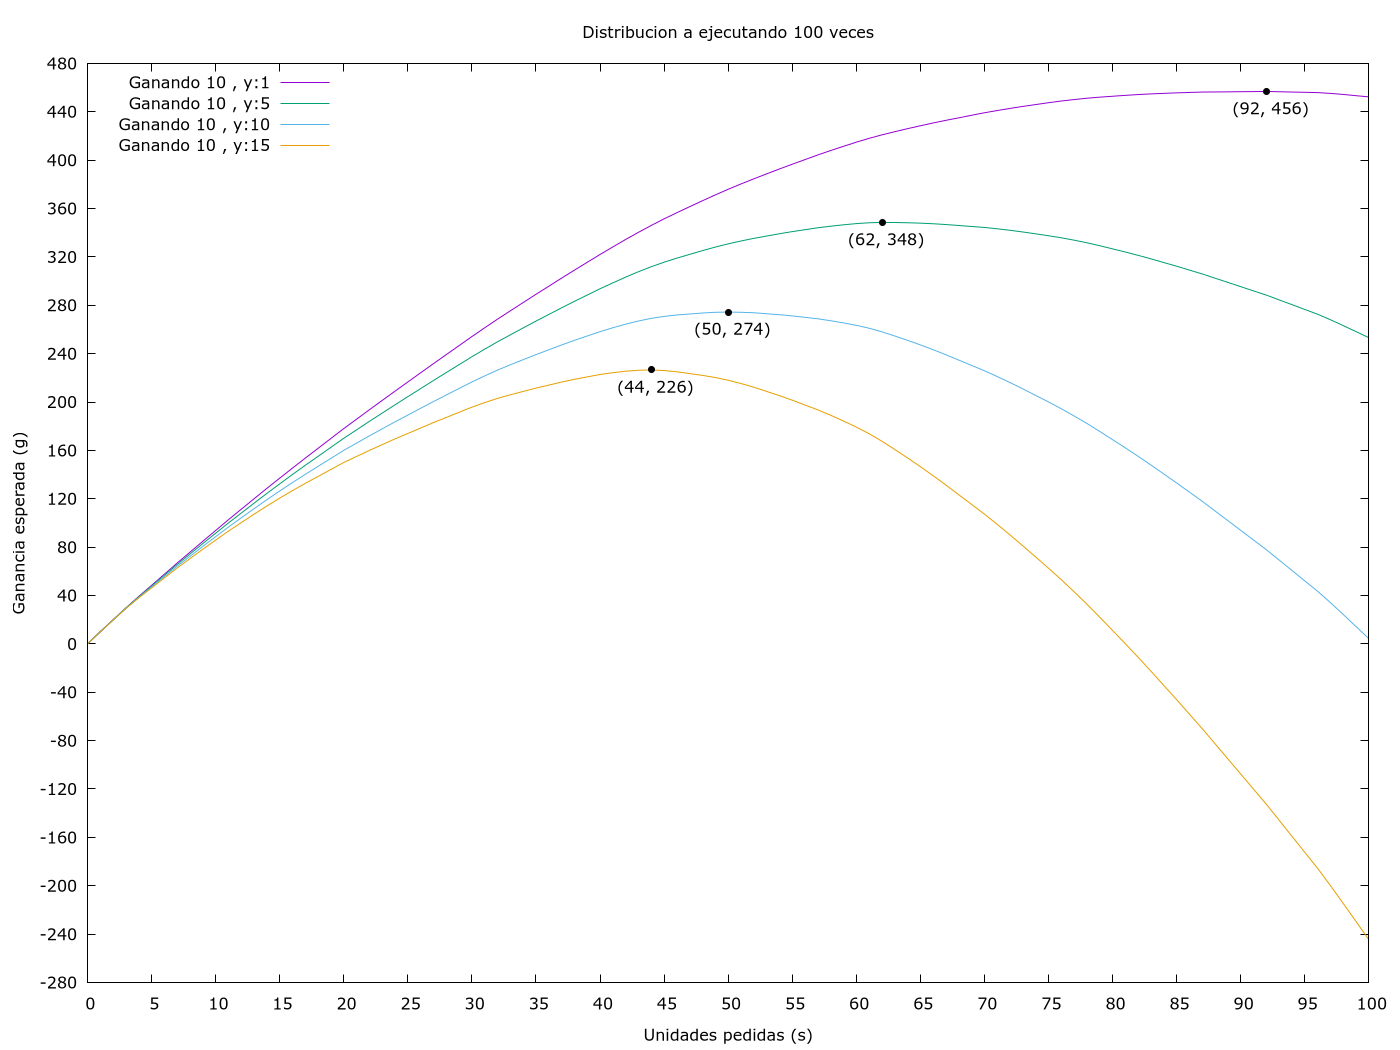
\includegraphics[scale = 0.2]{prob_a/datos_a_100.png}
	\caption{Con 100 repeticiones y la distribución a.}
	\label{fig:ej1_a_100}

\end{figure}

\begin{figure}[H]
	\centering
	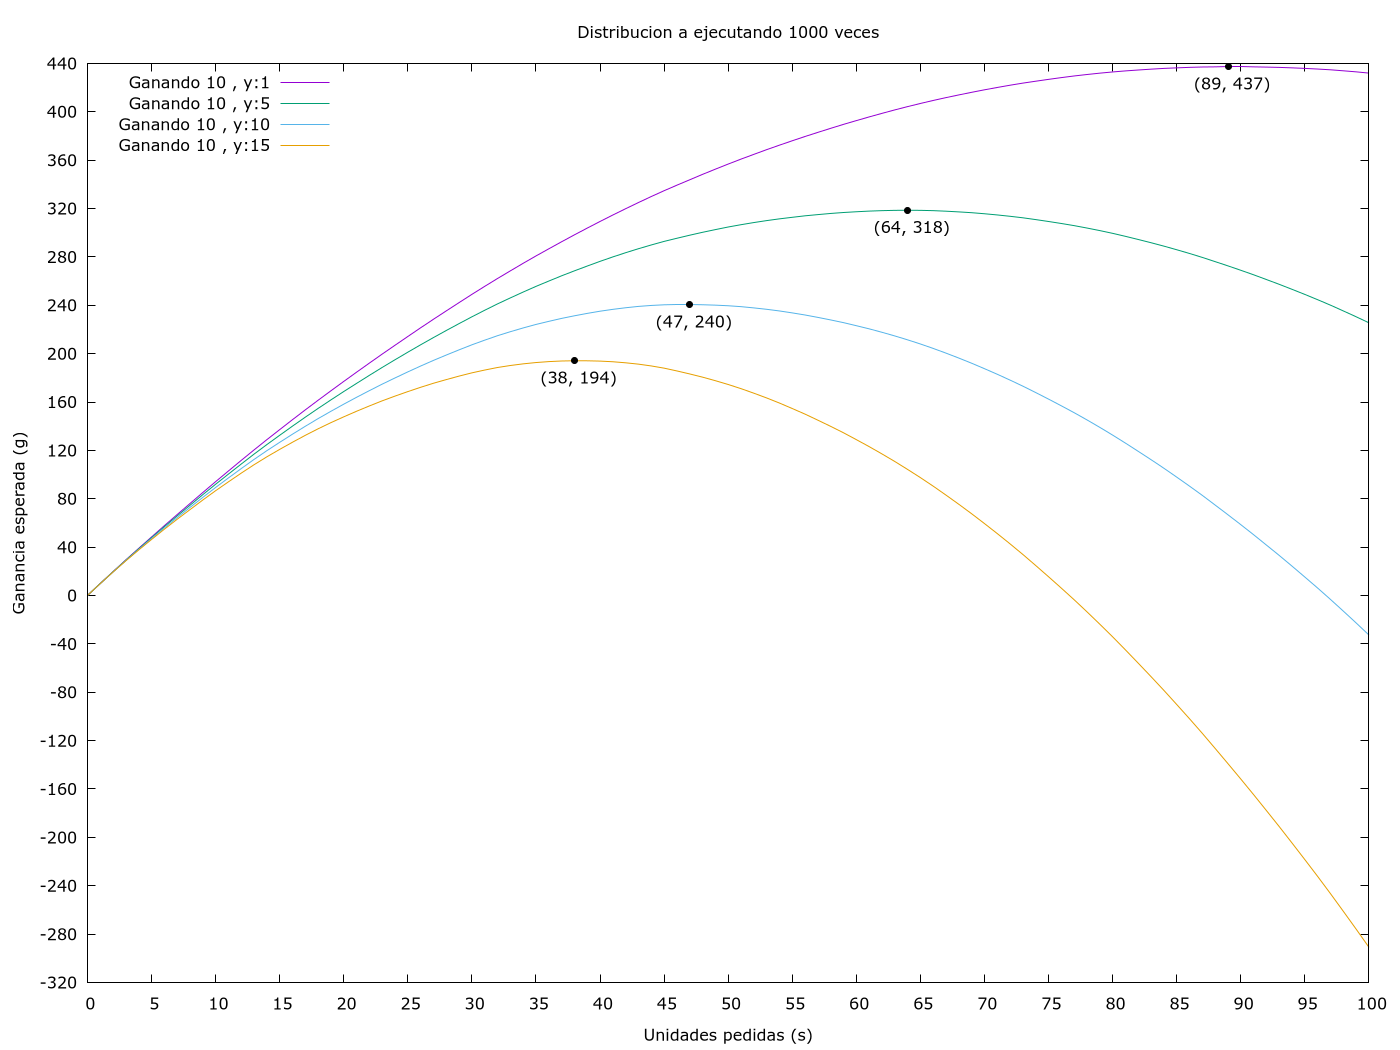
\includegraphics[scale = 0.2]{prob_a/datos_a_1000.png}
	\caption{Con 1000 repeticiones y la distribución a.}
	\label{fig:ej1_a_1000}

\end{figure}

\begin{figure}[H]
	\centering
	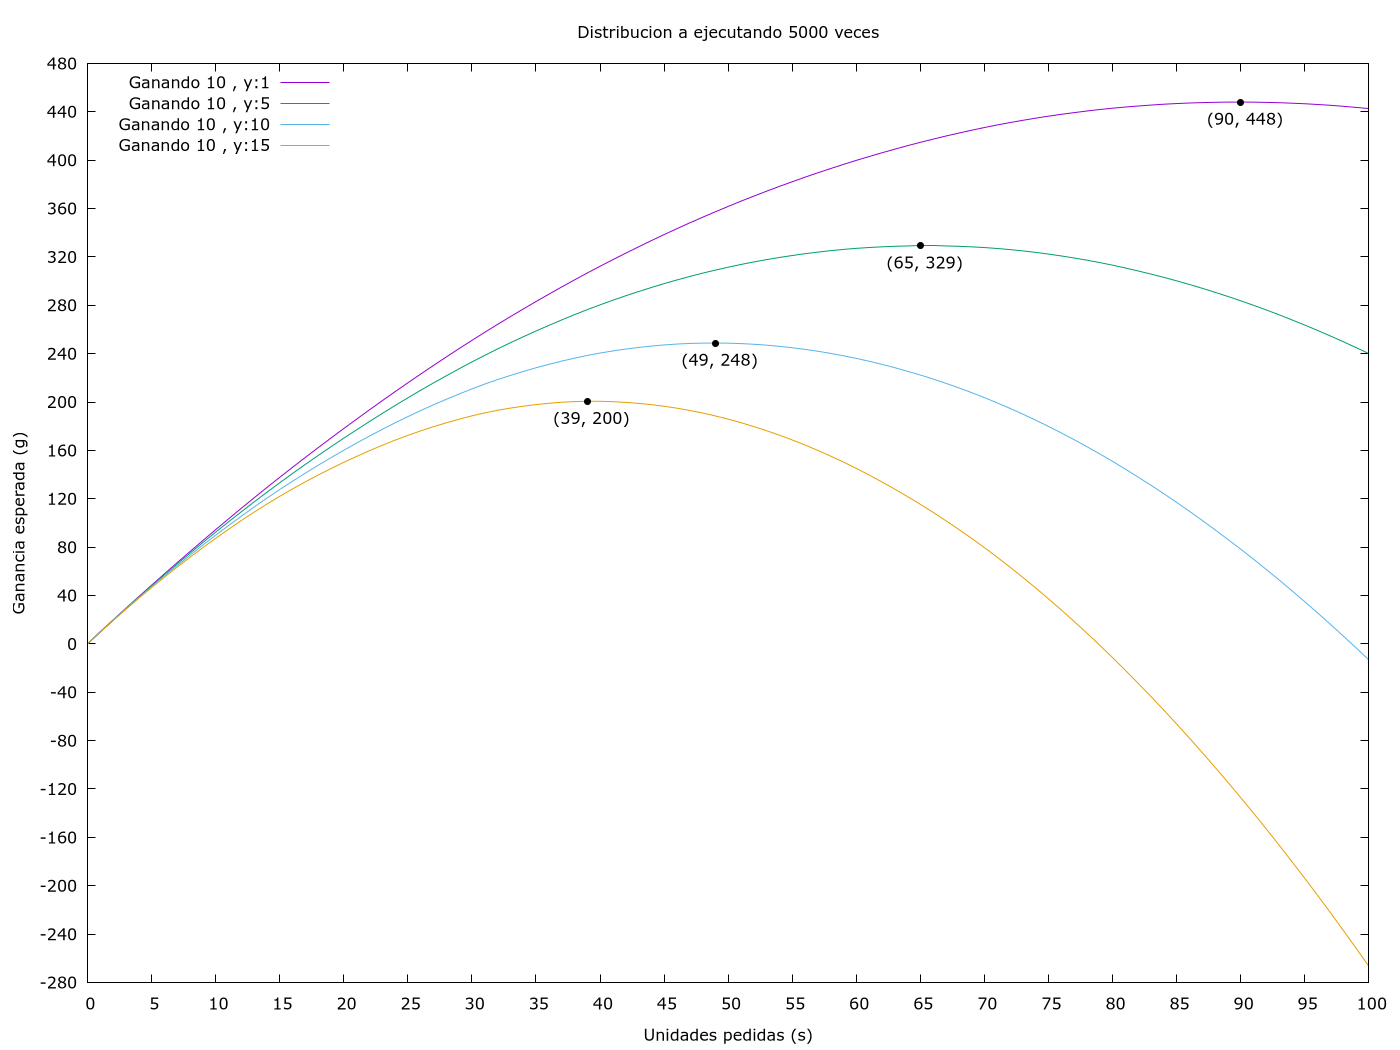
\includegraphics[scale = 0.2]{prob_a/datos_a_5000.png}
	\caption{Con 5000 repeticiones y la distribución a.}
	\label{fig:ej1_a_5000}

\end{figure}


\begin{figure}[H]
	\centering
	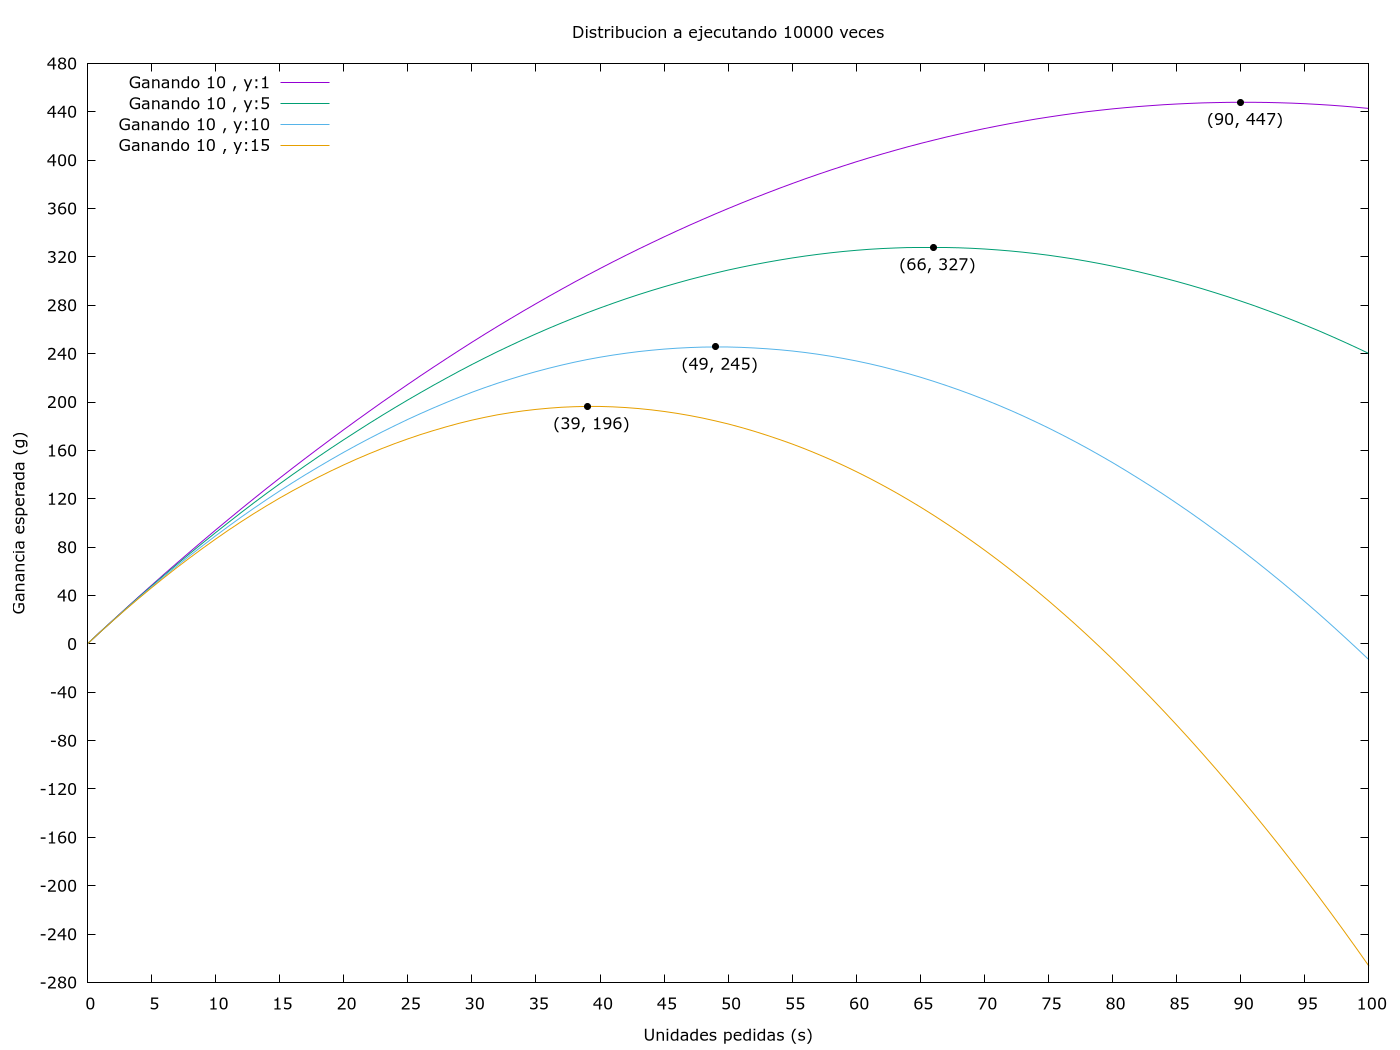
\includegraphics[scale = 0.2]{prob_a/datos_a_10000.png}
	\caption{Con 10000 repeticiones y la distribución a.}
	\label{fig:ej1_a_10000}

\end{figure}

\begin{figure}[H]
	\centering
	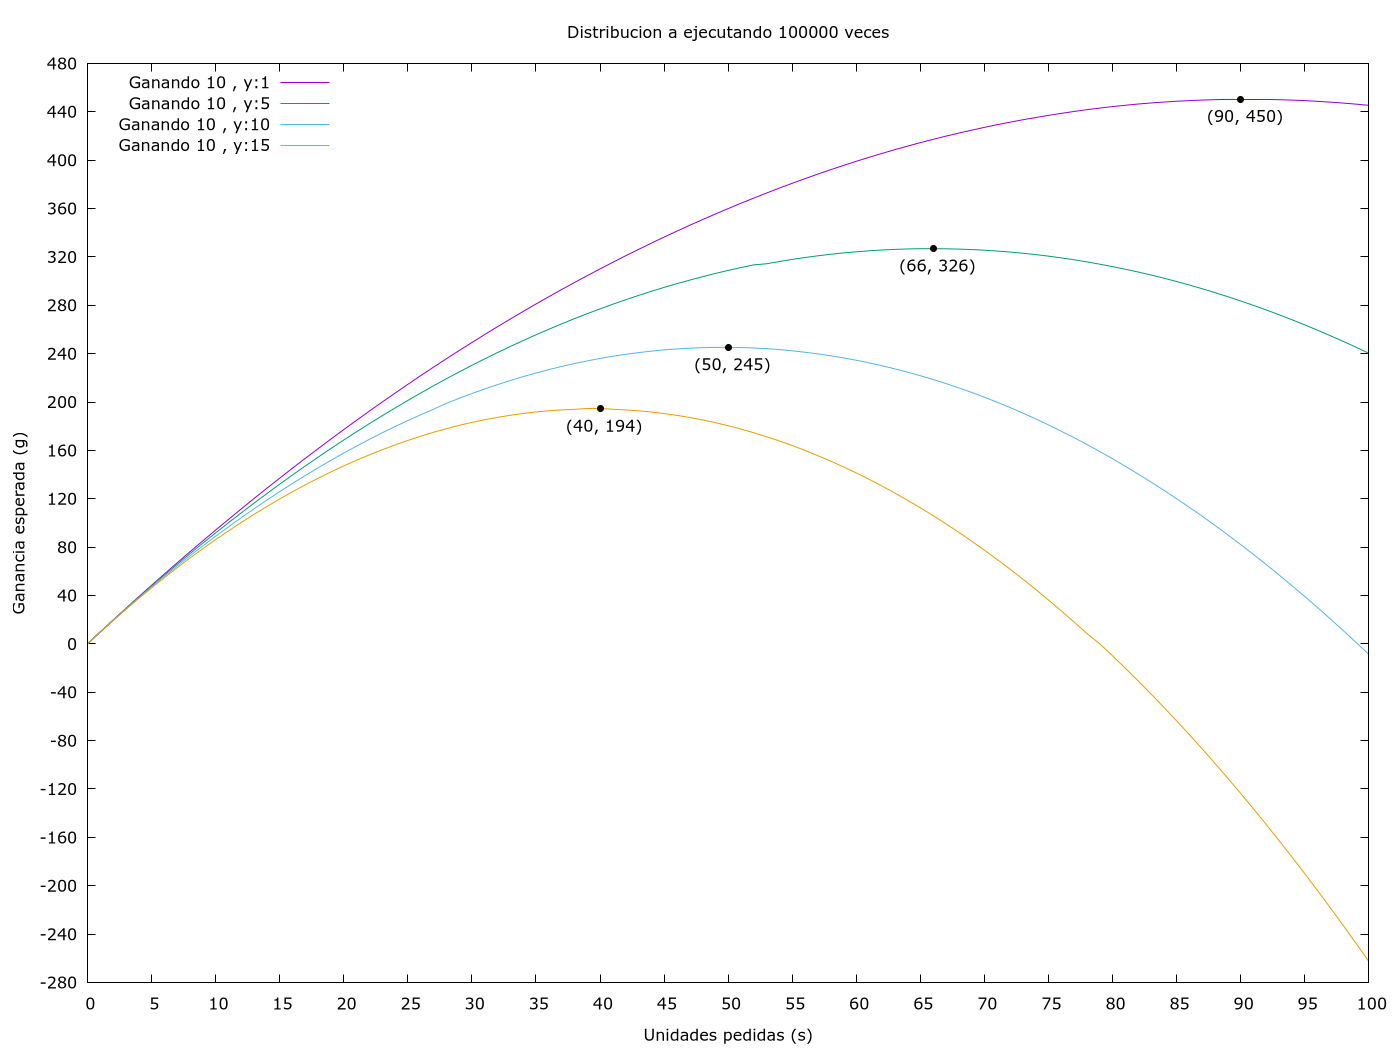
\includegraphics[scale = 0.2]{prob_a/datos_a_100000.png}
	\caption{Con 100000 repeticiones y la distribución a.}
	\label{fig:ej1_a_100000}

\end{figure}

\begin{figure}[H]
	\centering
	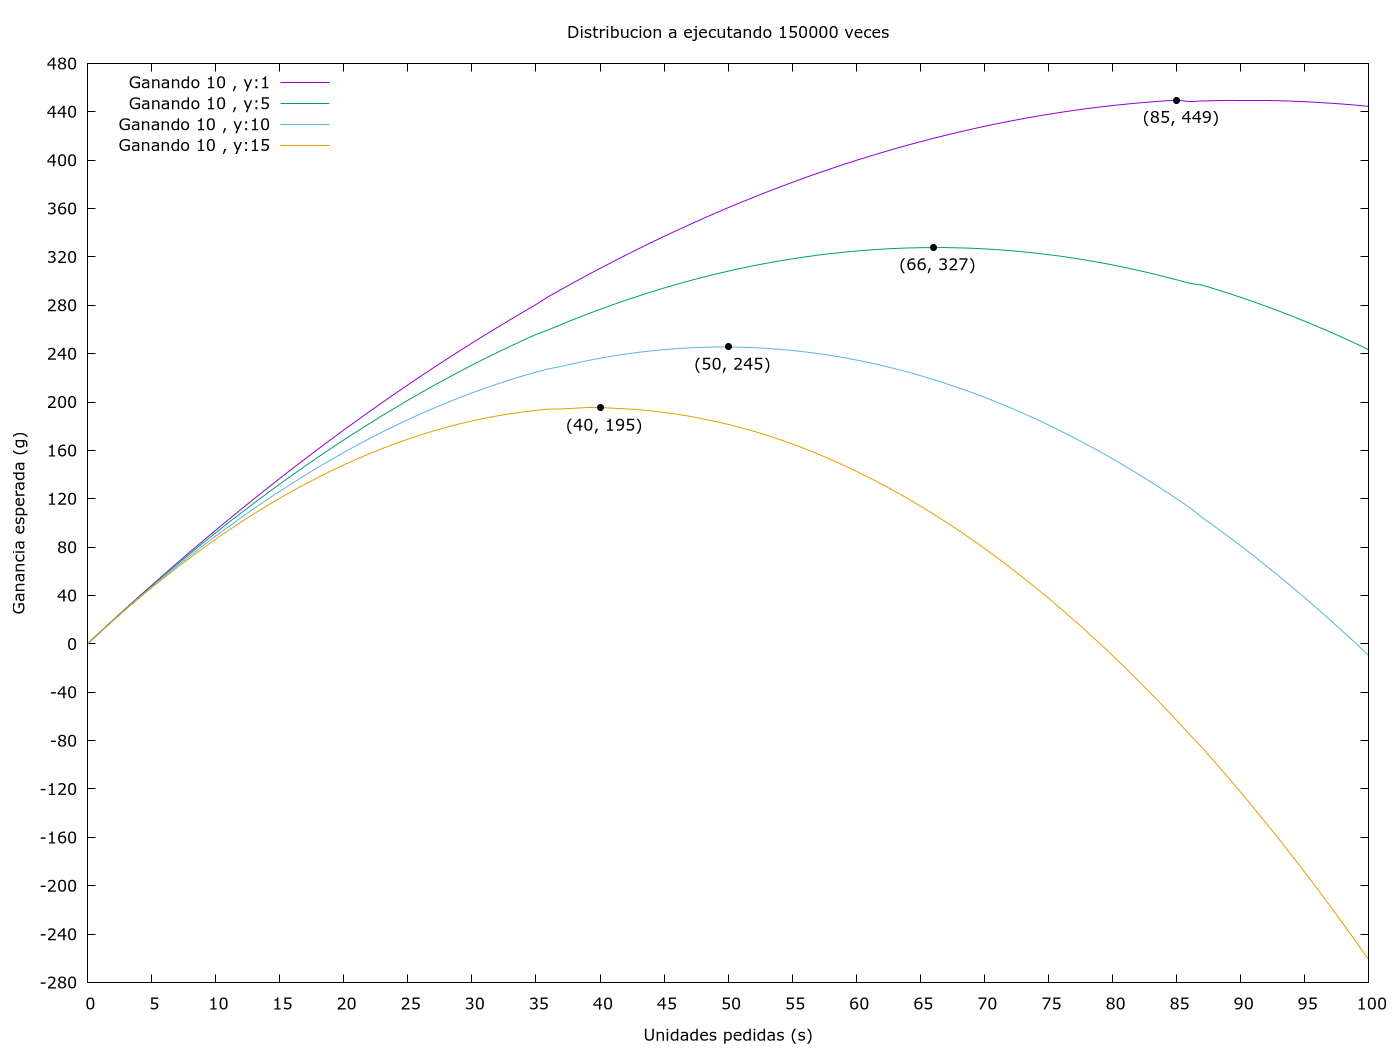
\includegraphics[scale = 0.2]{prob_a/datos_a_150000.png}
	\caption{Con 150000 repeticiones y la distribución a.}
	\label{fig:ej1_a_150000}

\end{figure}

En estas gráficas vemos como al ejecutar con distinto número de repeticiones, a mayor número de repeticiones se acerca más al óptimo calculado en el guión de la práctica hasta alcanzarlo, además de que en todas las gráficas, a una mayor perdida por unidad no vendida la ganancia máxima va siendo más baja y el óptimo de periódicos a contratar se acerca a cero, por lo que es el comportamiento esperado del sistema.

En este caso, en el que cualquier valor de demanda tiene la misma probabilidad de aparecer, vemos como solo llegan a producirse perdidas en los casos más extremos en los que por cada periódico vendido se pierde lo mismo o más que lo que ganamos por el periódico, por lo que esta es una situación favorable ya que esto casi nunca ocurre.


\subsubsection{Resultados obtenidos con la distribución b}

La distribución b se basa en una distribución de probabilidad proporcional siguiendo $100 - d$, es decir, los valores más pequeños de d tendrán más probabilidades de aparecer.

\begin{figure}[H]
	\centering
	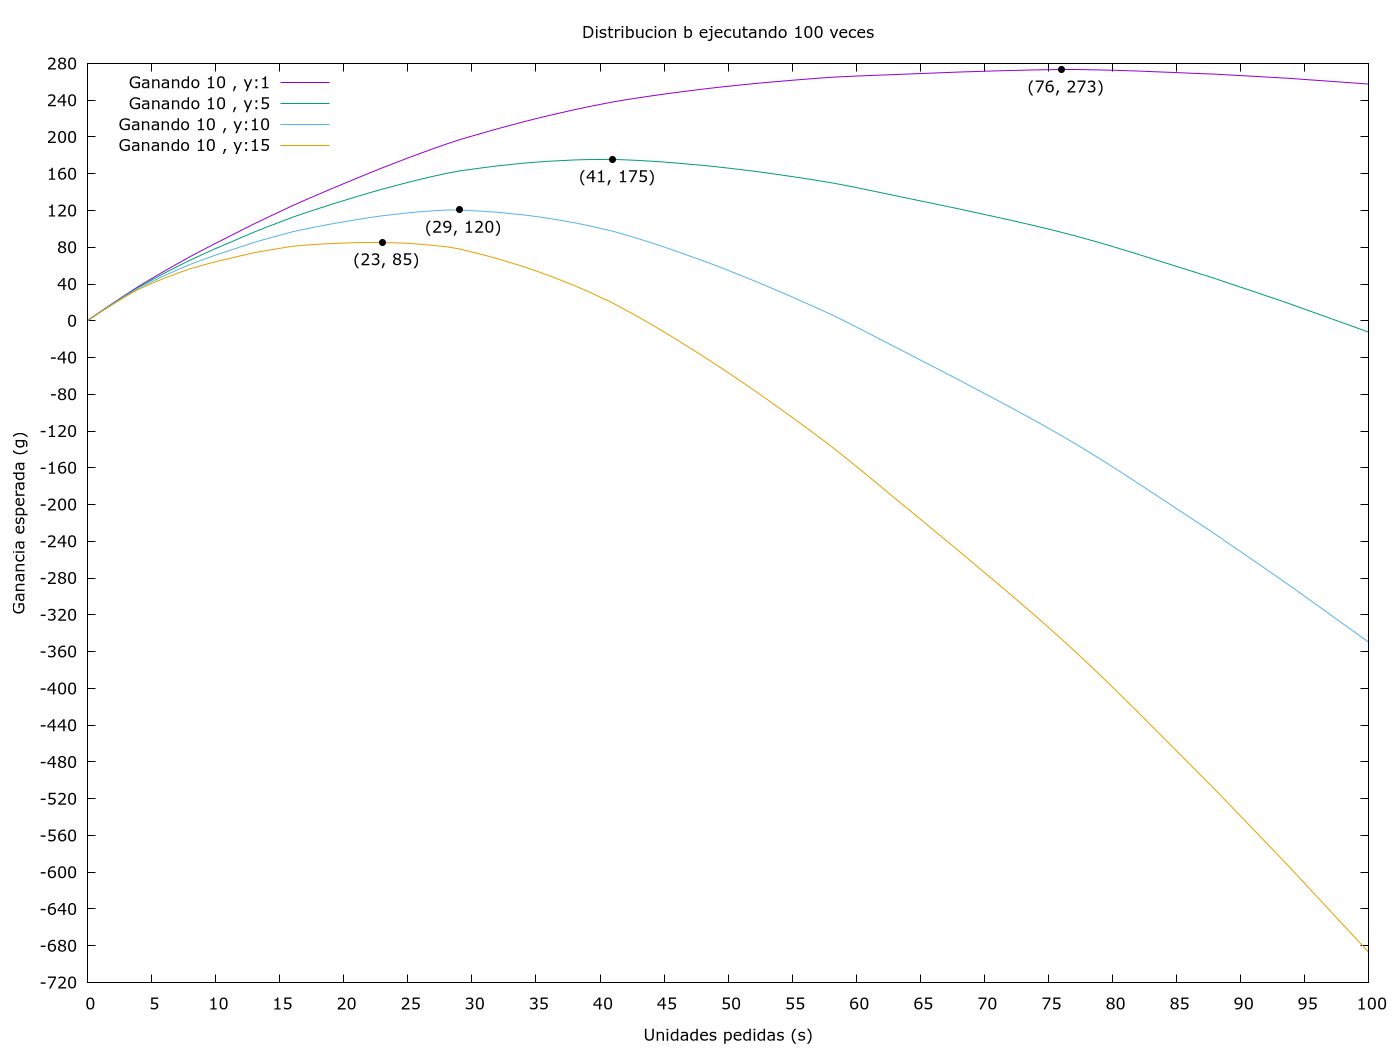
\includegraphics[scale = 0.2]{prob_b/datos_b_100.png}
	\caption{Con 100 repeticiones y la distribución b.}
	\label{fig:ej1_a_100}

\end{figure}

\begin{figure}[H]
	\centering
	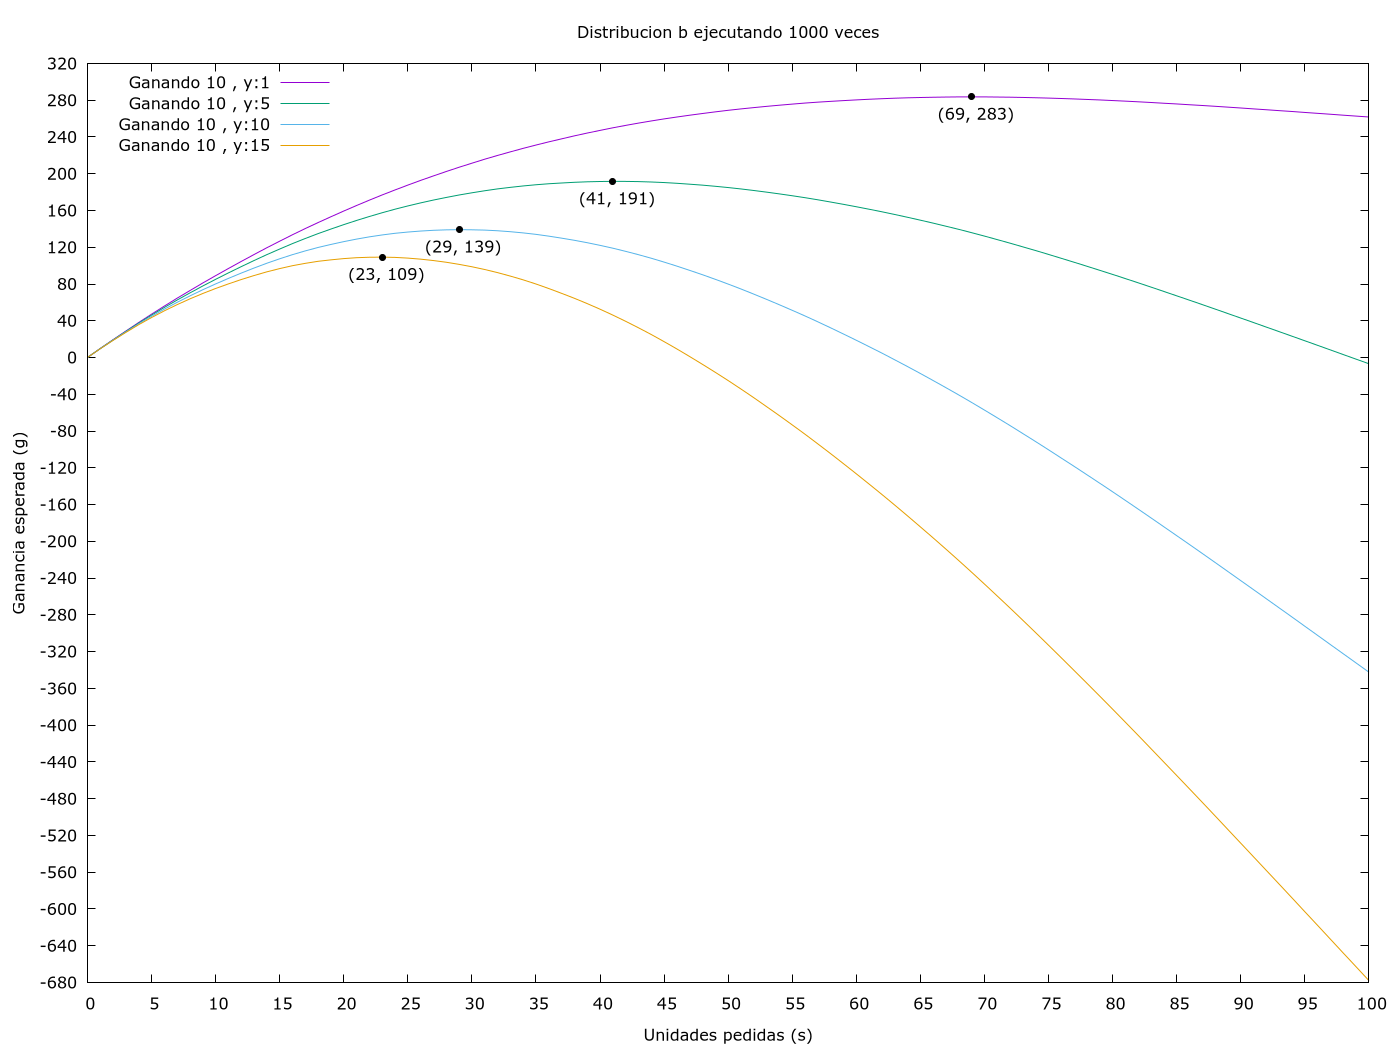
\includegraphics[scale = 0.2]{prob_b/datos_b_1000.png}
	\caption{Con 1000 repeticiones y la distribución b.}
	\label{fig:ej1_a_1000}

\end{figure}

\begin{figure}[H]
	\centering
	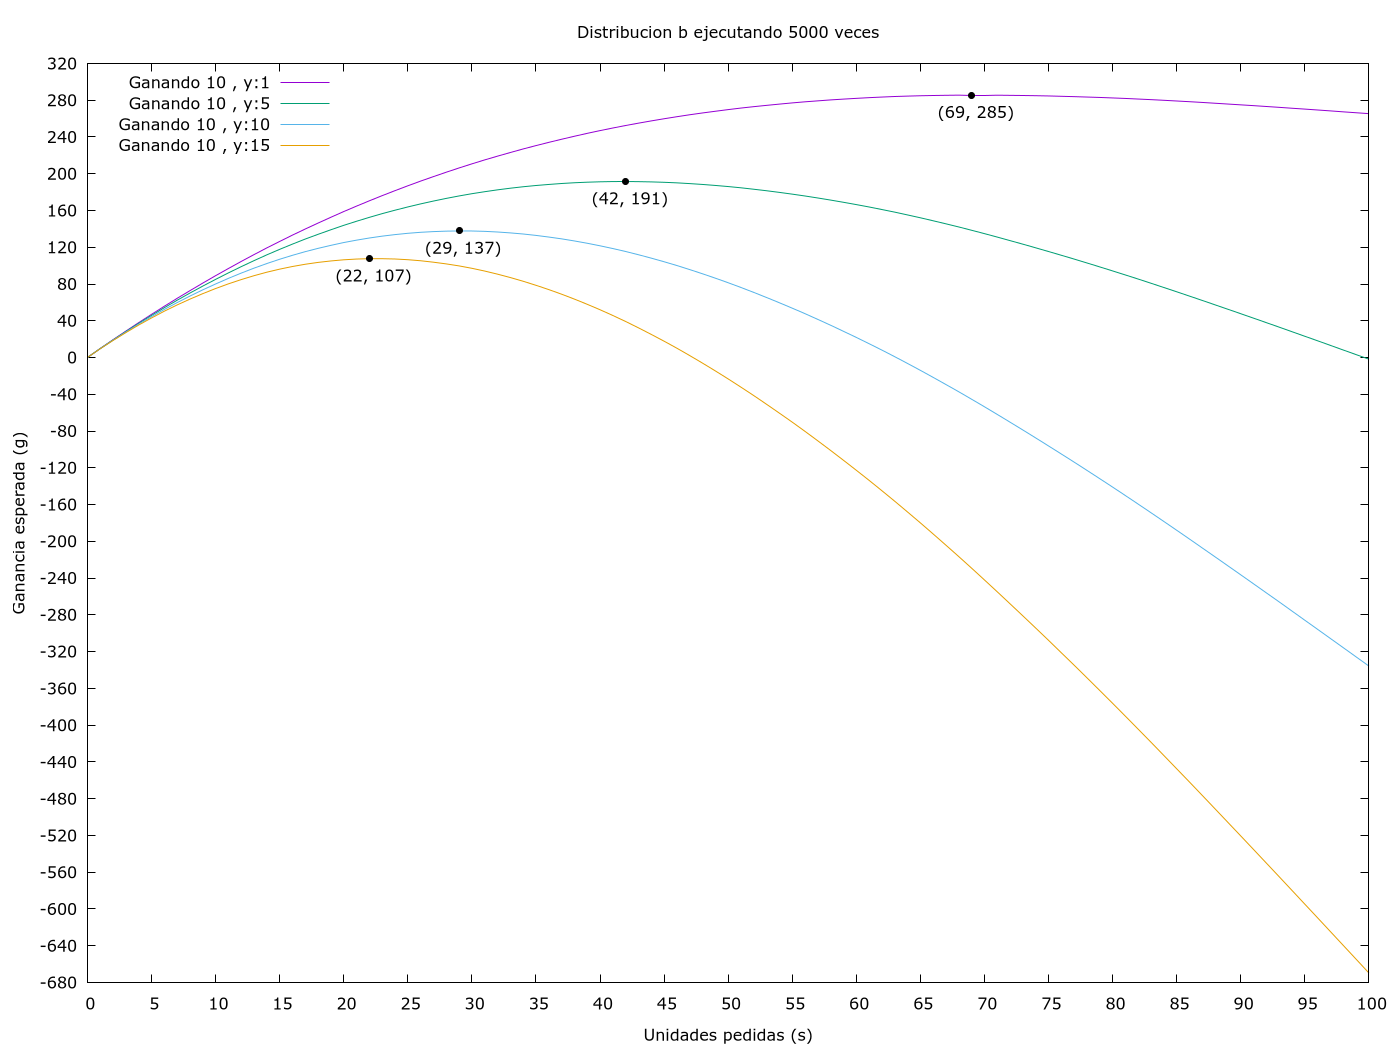
\includegraphics[scale = 0.2]{prob_b/datos_b_5000.png}
	\caption{Con 5000 repeticiones y la distribución b.}
	\label{fig:ej1_a_5000}

\end{figure}


\begin{figure}[H]
	\centering
	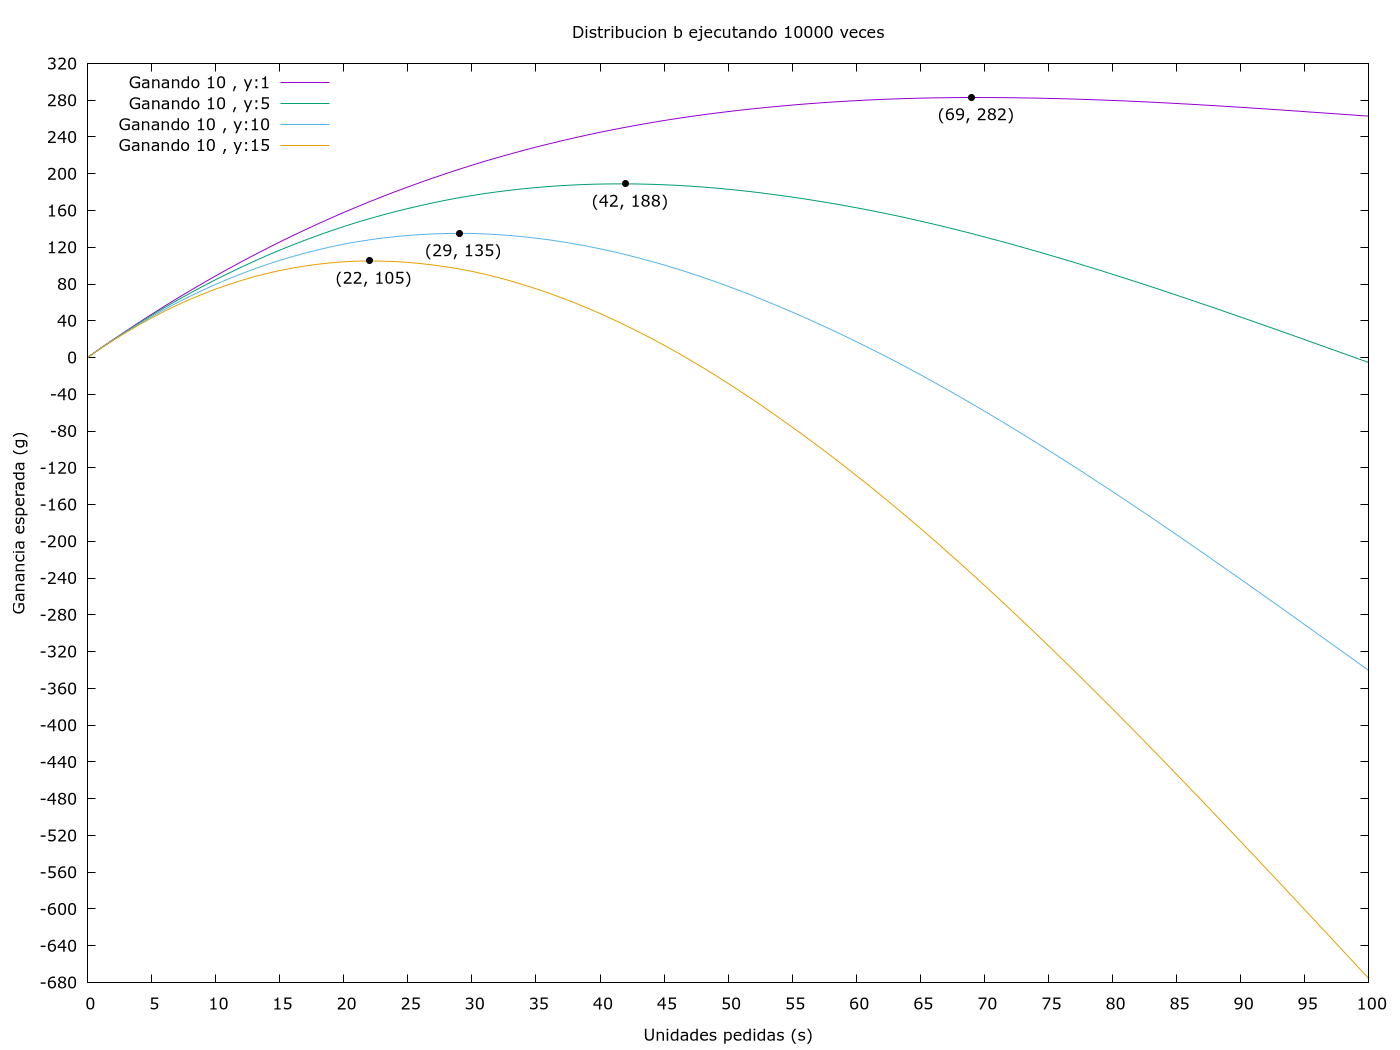
\includegraphics[scale = 0.2]{prob_b/datos_b_10000.png}
	\caption{Con 10000 repeticiones y la distribución b.}
	\label{fig:ej1_a_10000}

\end{figure}

\begin{figure}[H]
	\centering
	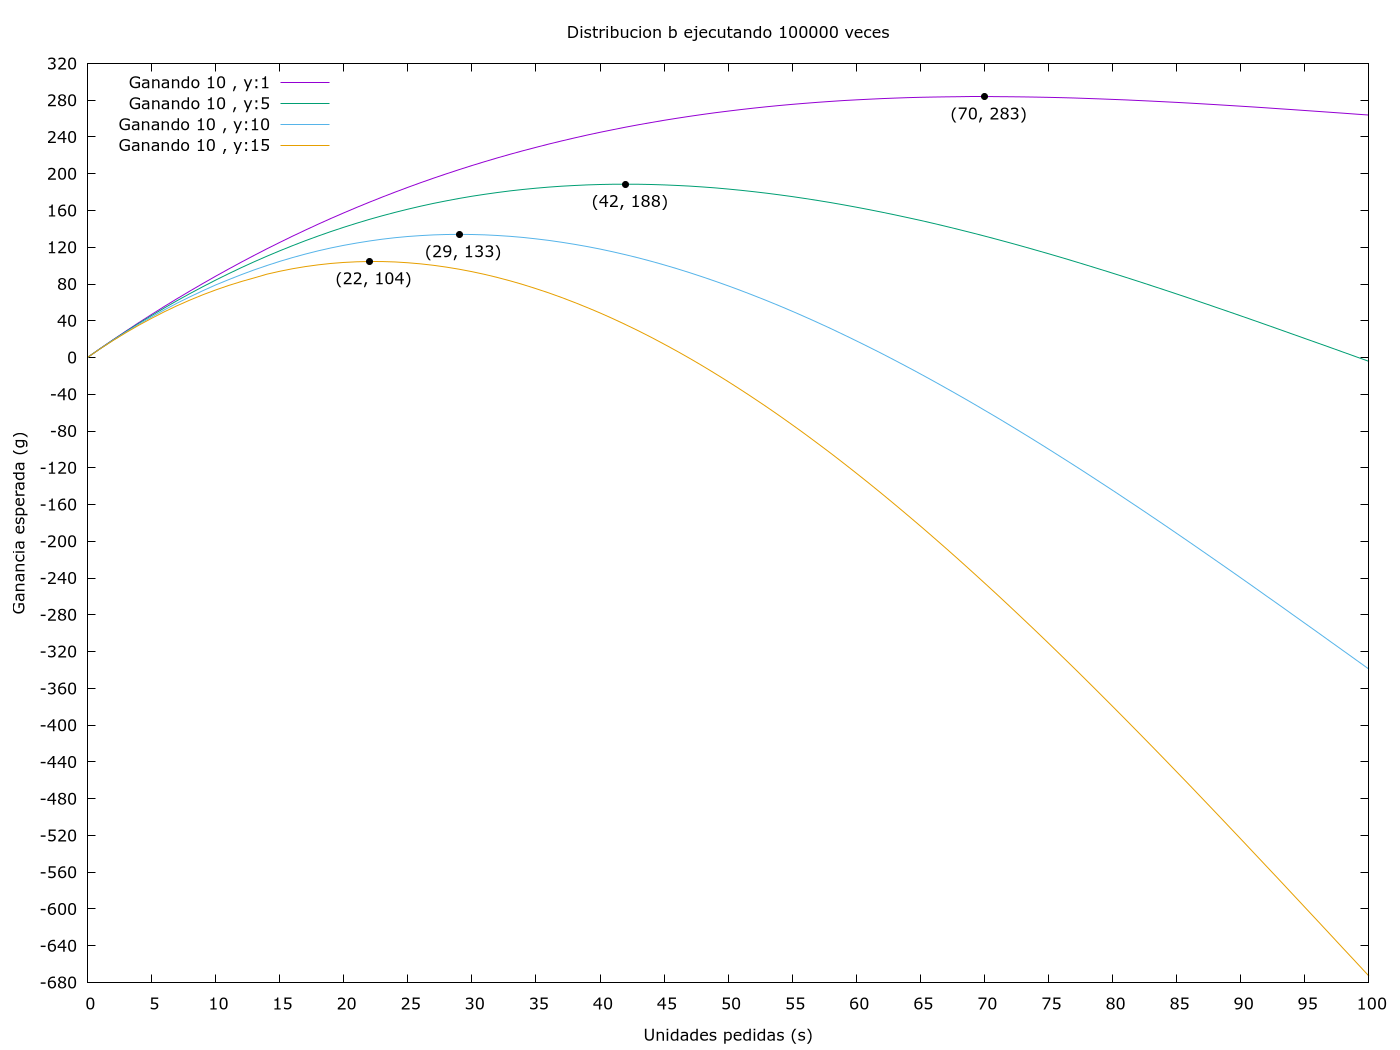
\includegraphics[scale = 0.2]{prob_b/datos_b_100000.png}
	\caption{Con 100000 repeticiones y la distribución b.}
	\label{fig:ej1_a_100000}

\end{figure}

\begin{figure}[H]
	\centering
	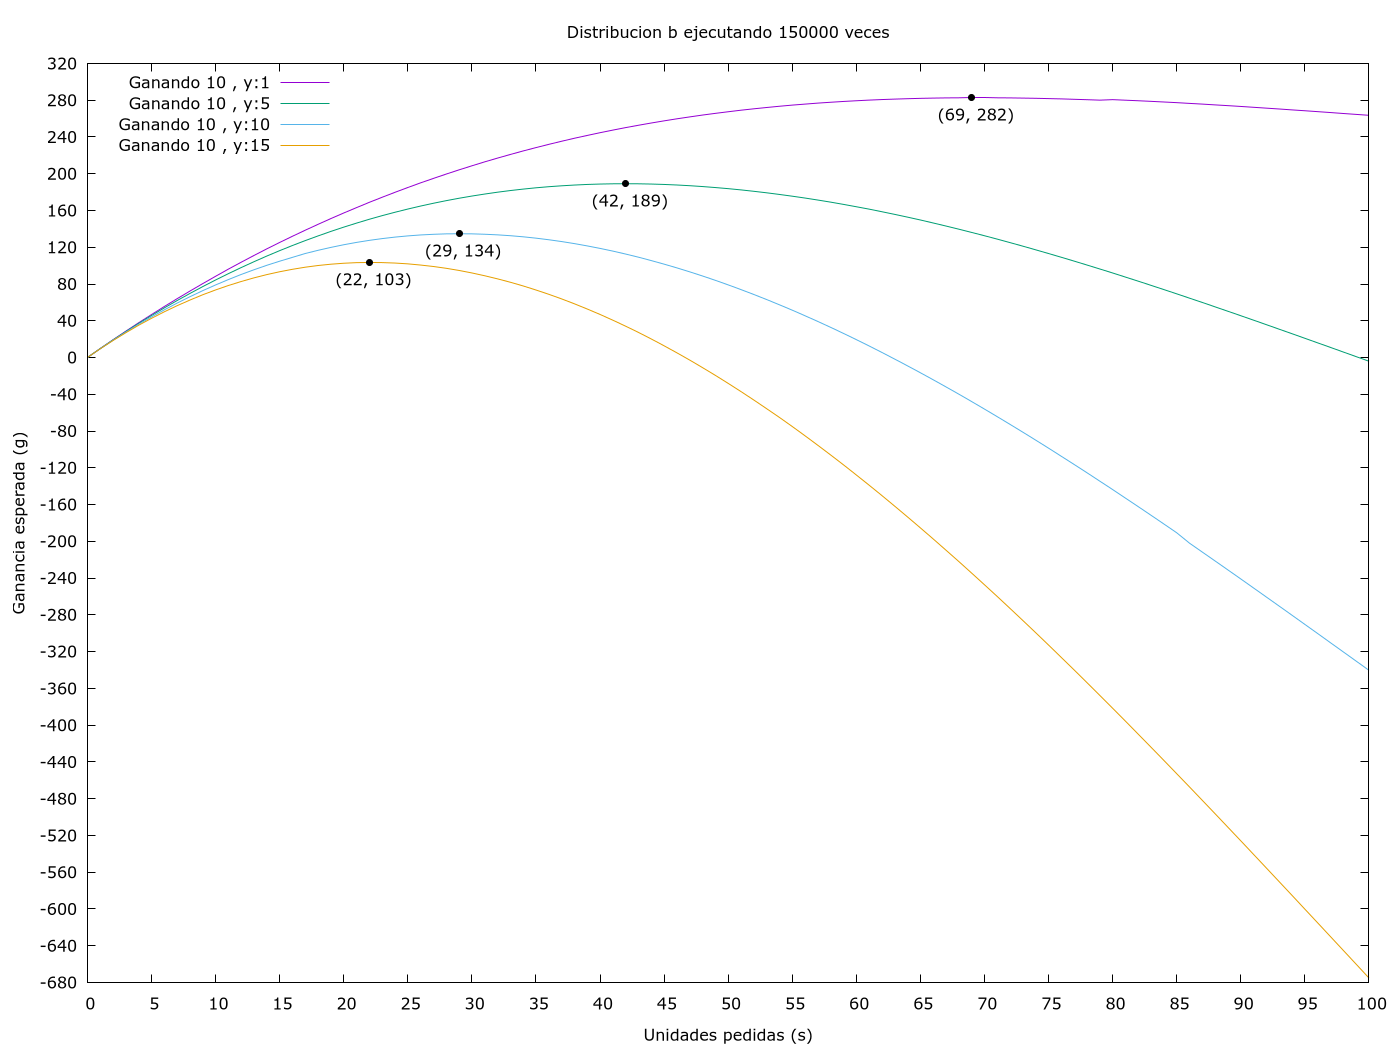
\includegraphics[scale = 0.2]{prob_b/datos_b_150000.png}
	\caption{Con 150000 repeticiones y la distribución b.}
	\label{fig:ej1_a_150000}

\end{figure}


Vemos como en este caso, en comparación con el caso a, los valores óptimos se encuentran mucho más a la izquierda en el eje X ya que es menos probable el que neceitemos una demanda alta, además de que las pérdidas son mucho mayores en valores altos, ya que casi nunca necesitaremos tantos periódicos, por lo que podemos intuir que el funcionamiento es correcto y se acerca a lo esperado.


\subsubsection{Resultados obtenidos con la distribución c}


La distribución c se basa en una distribución de probabilidad triangular, en la que los valores cercanos a 0 y 100 tienen la menor probabilidad a aparecer y los valores cercanos a 50 son más probables.

\begin{figure}[H]
	\centering
	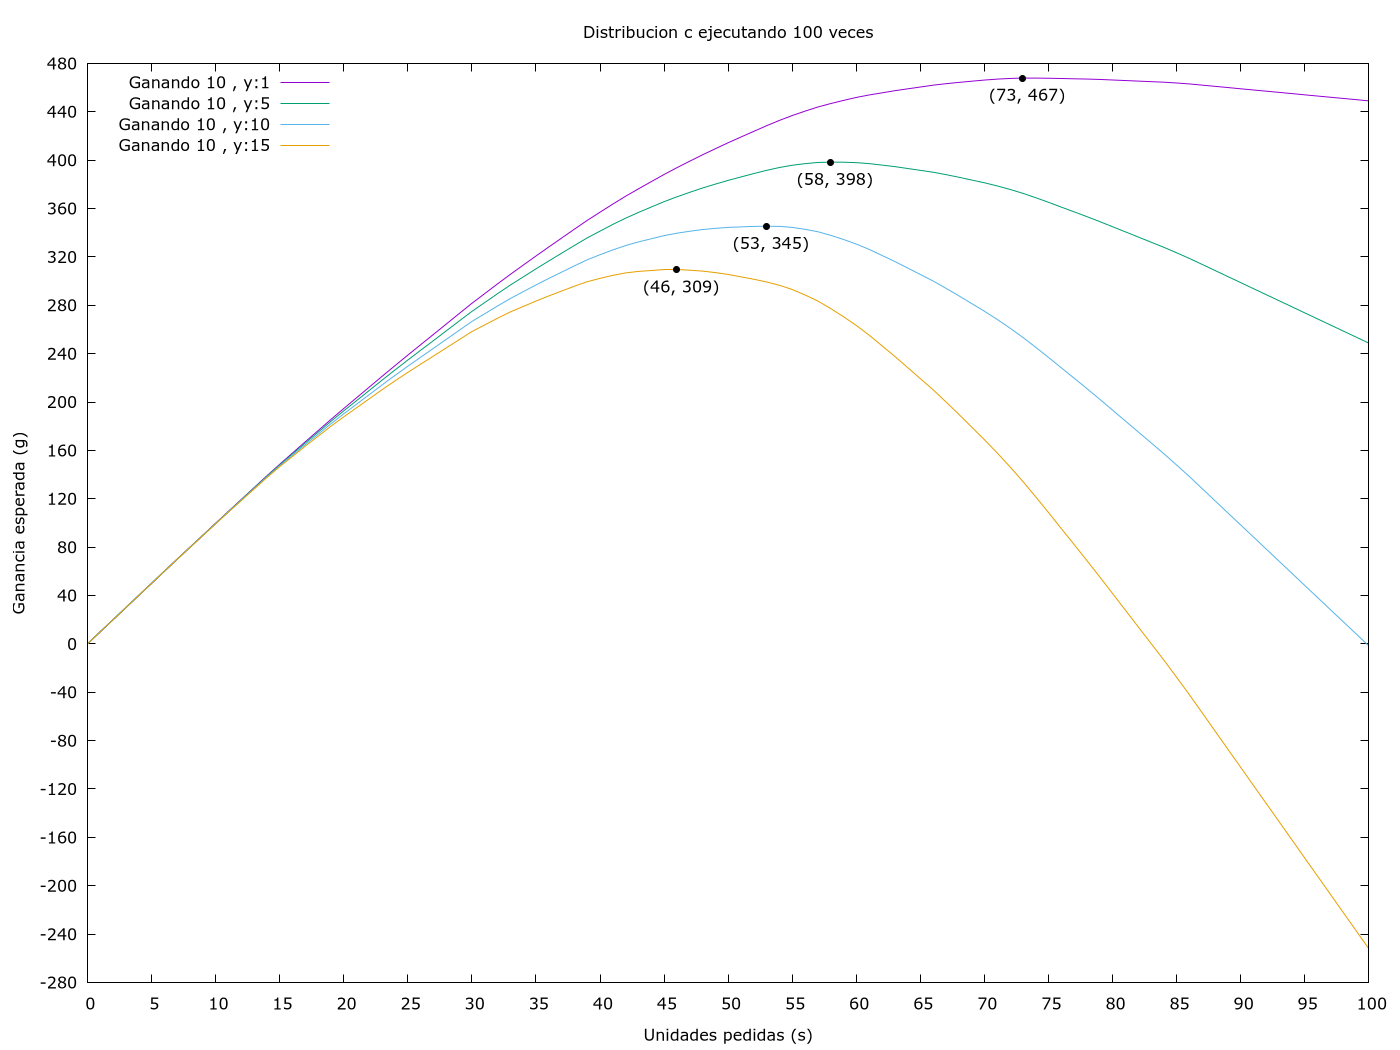
\includegraphics[scale = 0.2]{prob_c/datos_c_100.png}
	\caption{Con 100 repeticiones y la distribución c.}
	\label{fig:ej1_a_100}

\end{figure}

\begin{figure}[H]
	\centering
	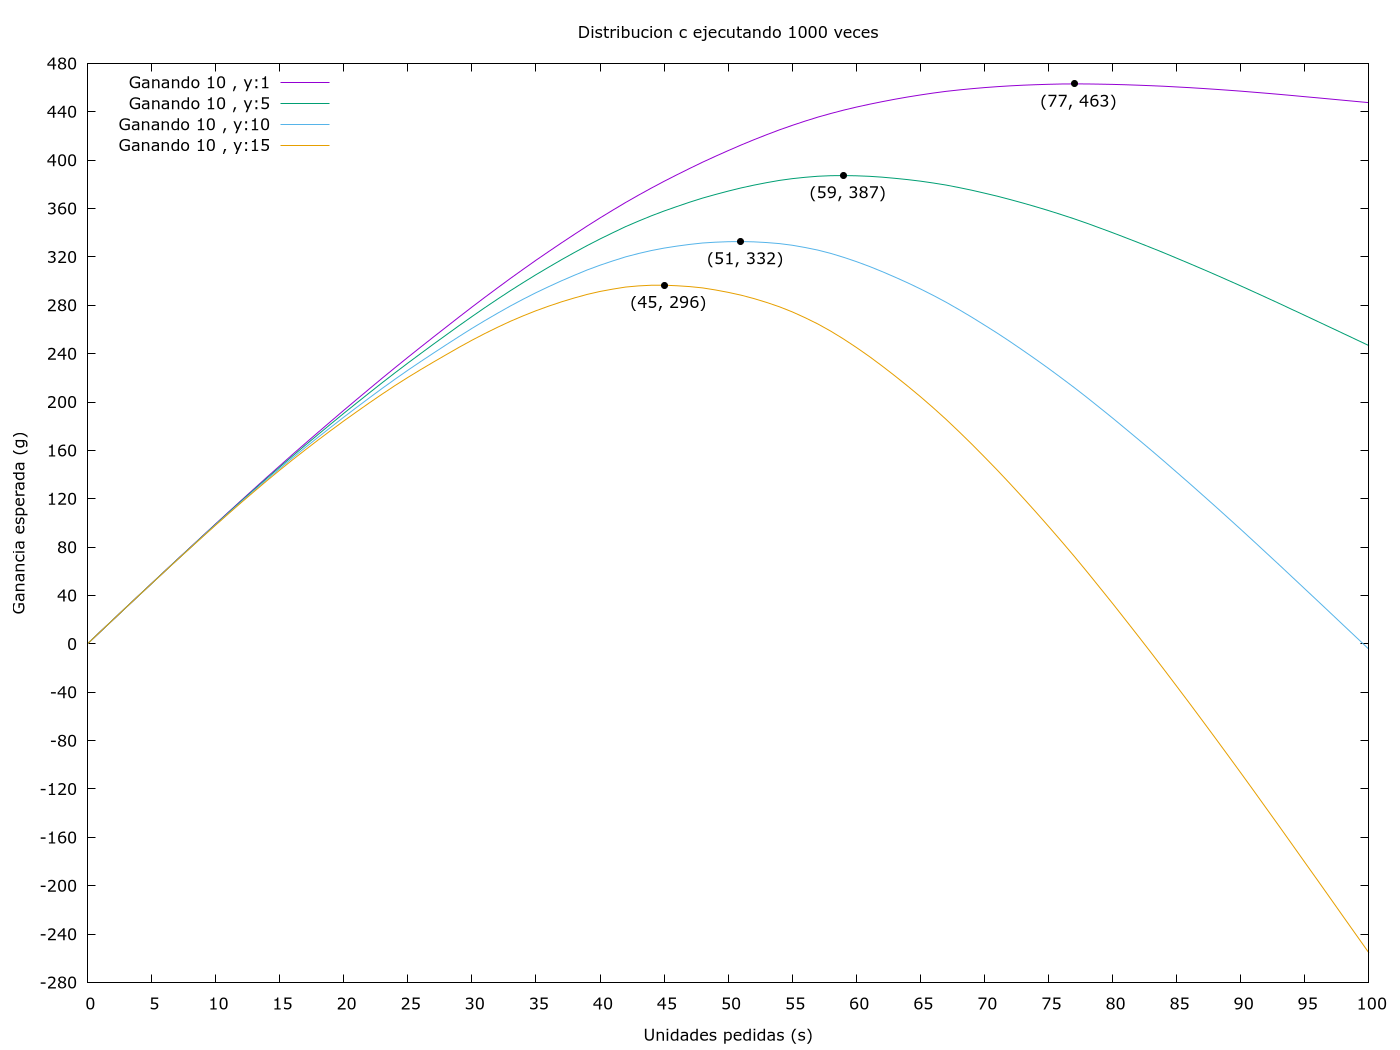
\includegraphics[scale = 0.2]{prob_c/datos_c_1000.png}
	\caption{Con 1000 repeticiones y la distribución c.}
	\label{fig:ej1_a_1000}

\end{figure}

\begin{figure}[H]
	\centering
	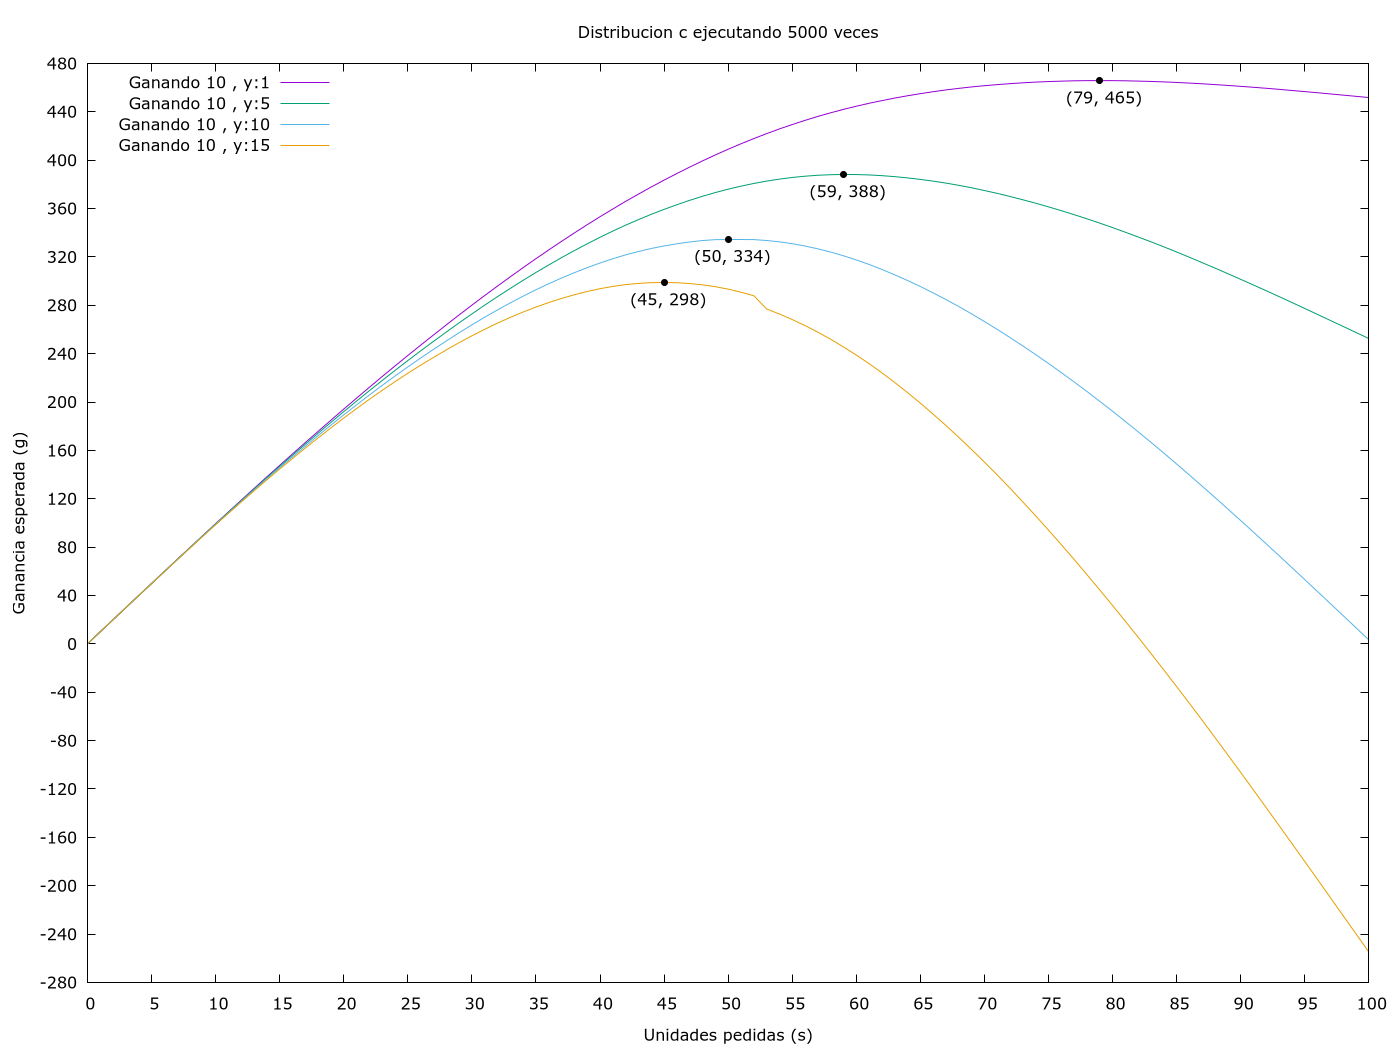
\includegraphics[scale = 0.2]{prob_c/datos_c_5000.png}
	\caption{Con 5000 repeticiones y la distribución c.}
	\label{fig:ej1_a_5000}

\end{figure}


\begin{figure}[H]
	\centering
	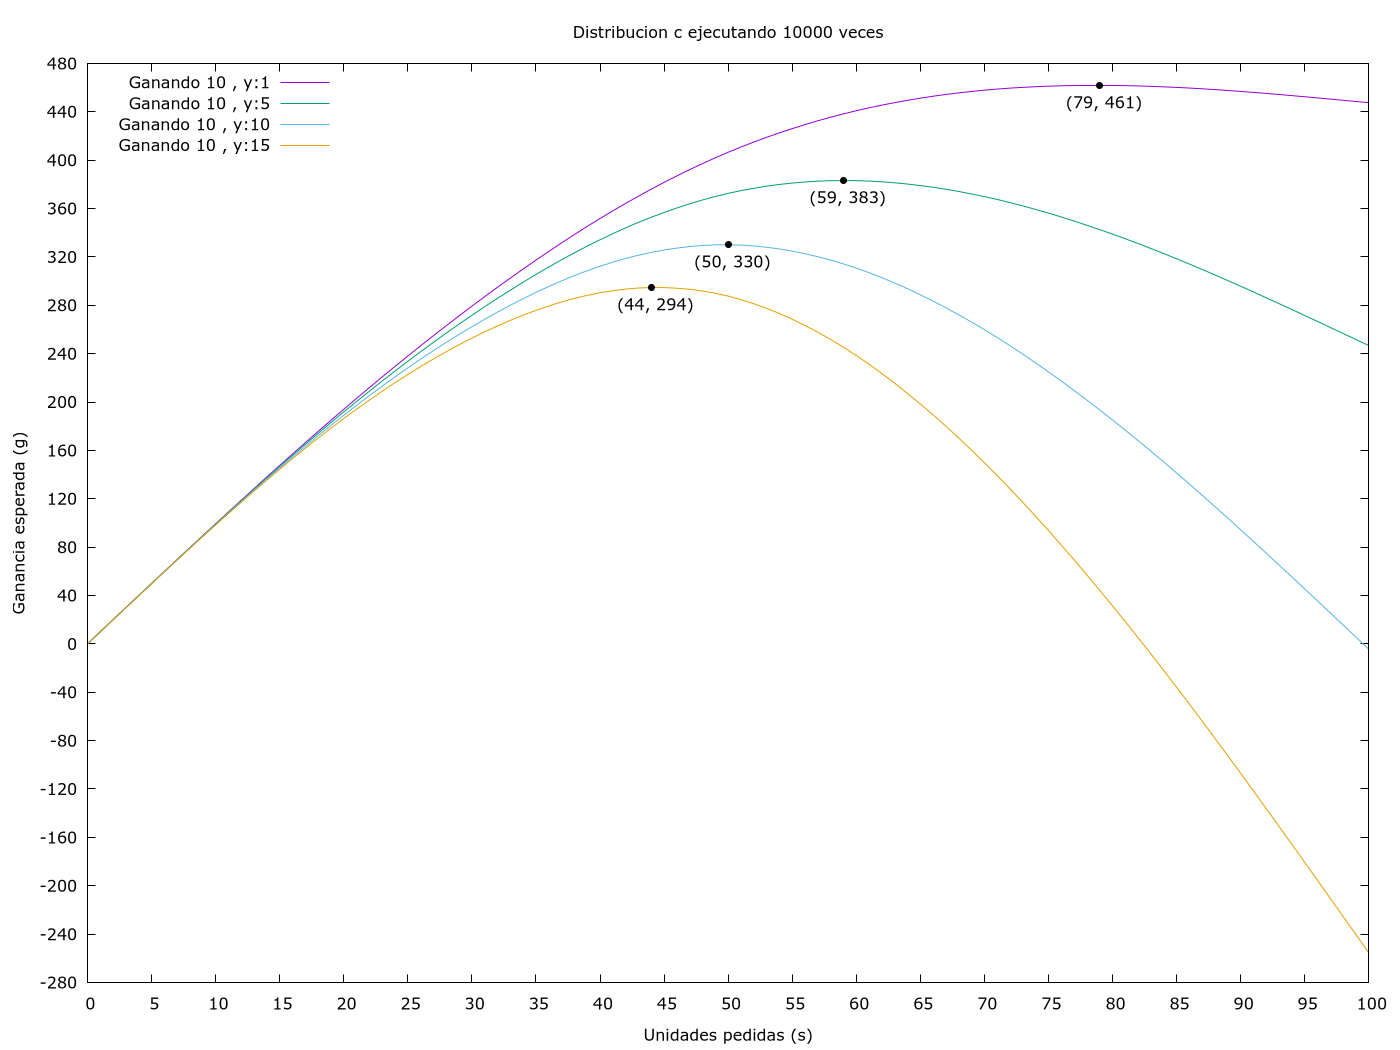
\includegraphics[scale = 0.2]{prob_c/datos_c_10000.png}
	\caption{Con 10000 repeticiones y la distribución c.}
	\label{fig:ej1_a_10000}

\end{figure}

\begin{figure}[H]
	\centering
	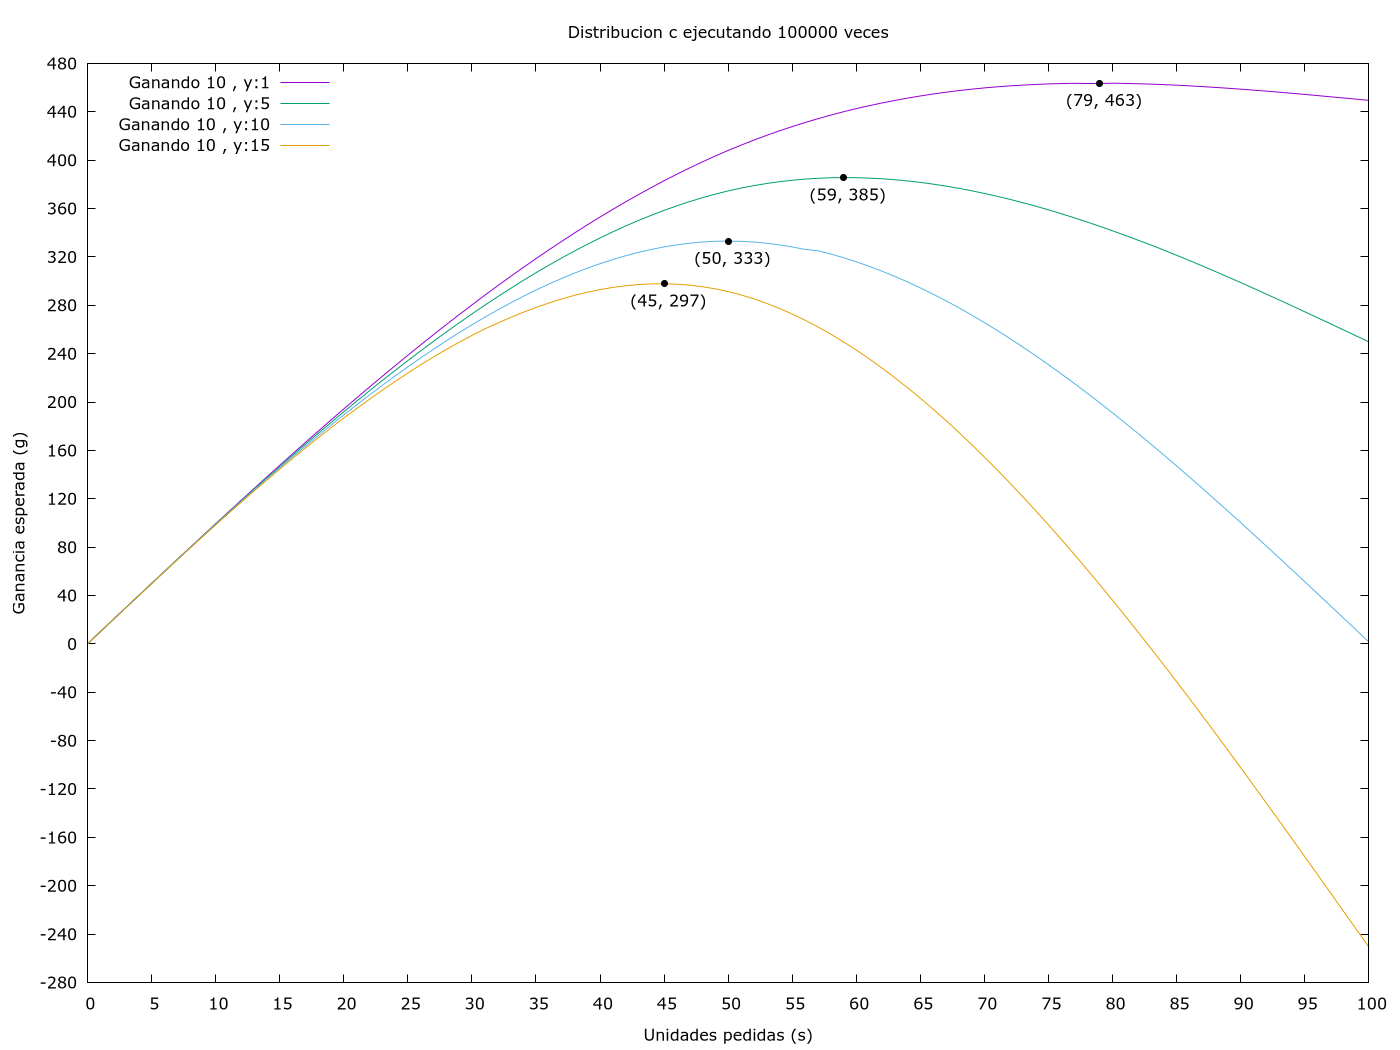
\includegraphics[scale = 0.2]{prob_c/datos_c_100000.png}
	\caption{Con 100000 repeticiones y la distribución c.}
	\label{fig:ej1_a_100000}

\end{figure}

\begin{figure}[H]
	\centering
	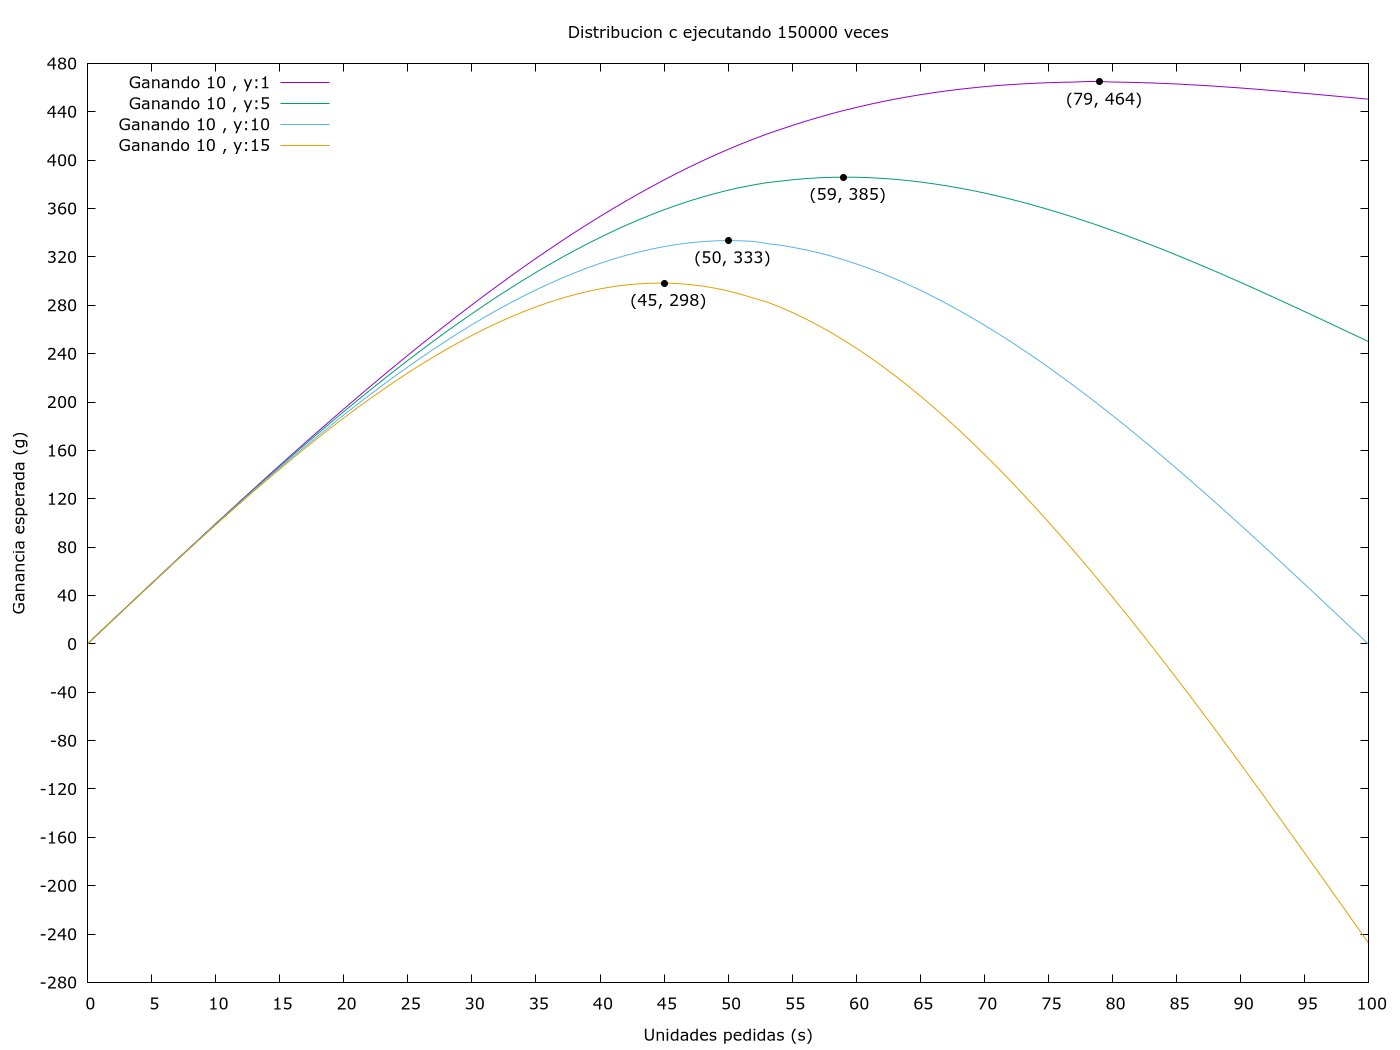
\includegraphics[scale = 0.2]{prob_c/datos_c_150000.png}
	\caption{Con 150000 repeticiones y la distribución c.}
	\label{fig:ej1_a_150000}

\end{figure}


\subsection{Modificación 1 del modelo}

\subsubsection{Resultados obtenidos con la distribución a}

\begin{figure}[H]
	\centering
	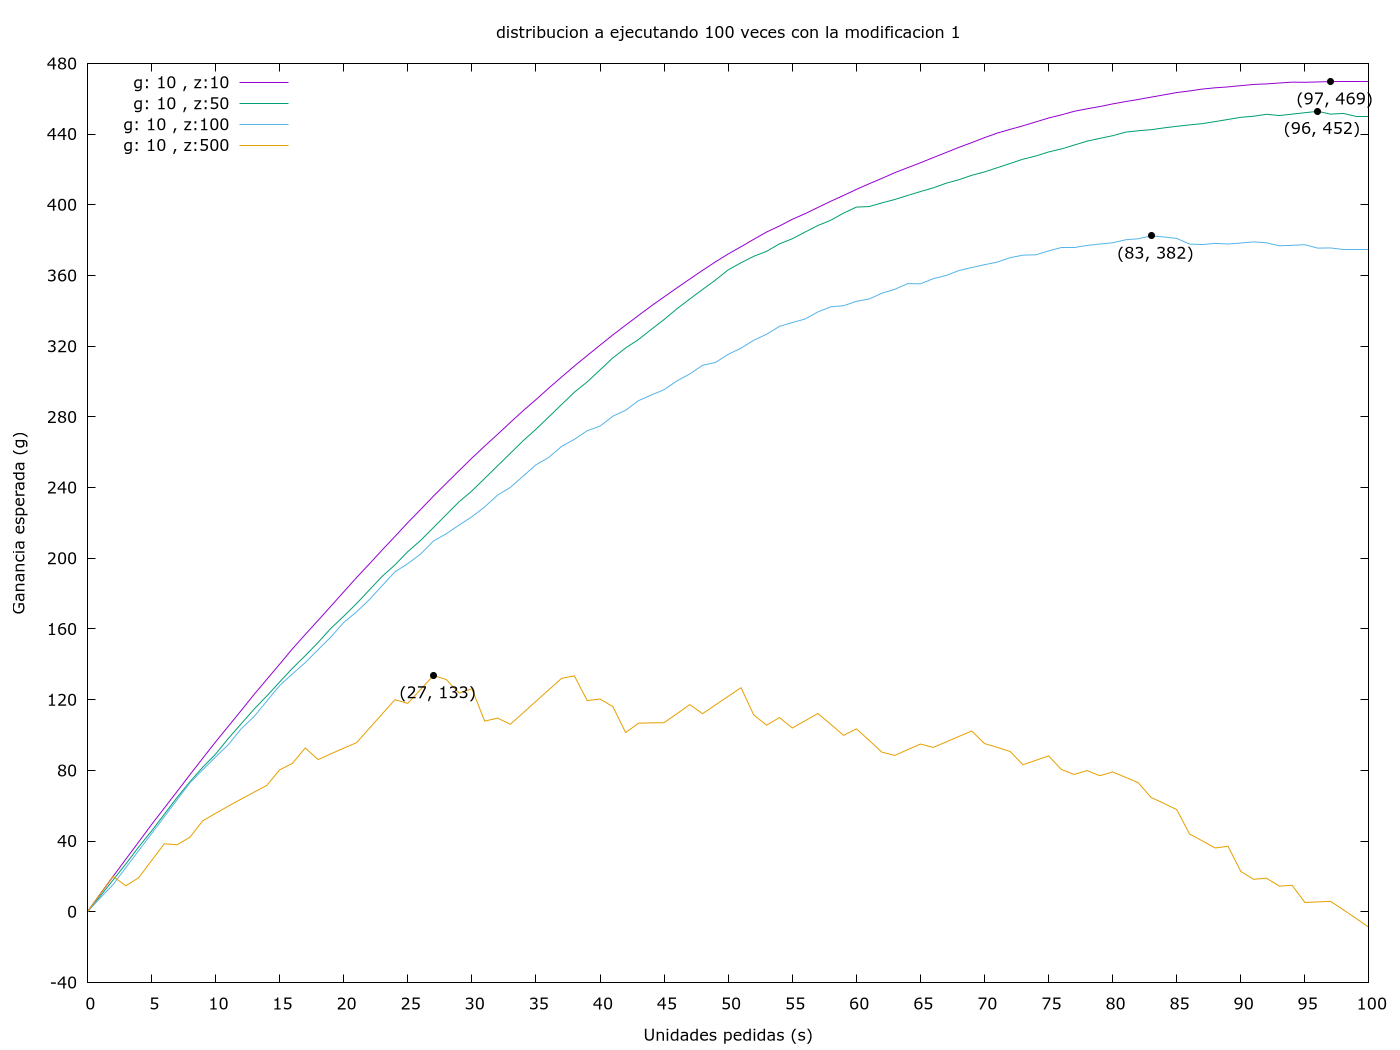
\includegraphics[scale = 0.2]{prob_a/datos_a_100_1.png}
	\caption{Con 100 repeticiones, la distribución a y la modificación 1.}
	\label{fig:ej1_a_100}

\end{figure}

\begin{figure}[H]
	\centering
	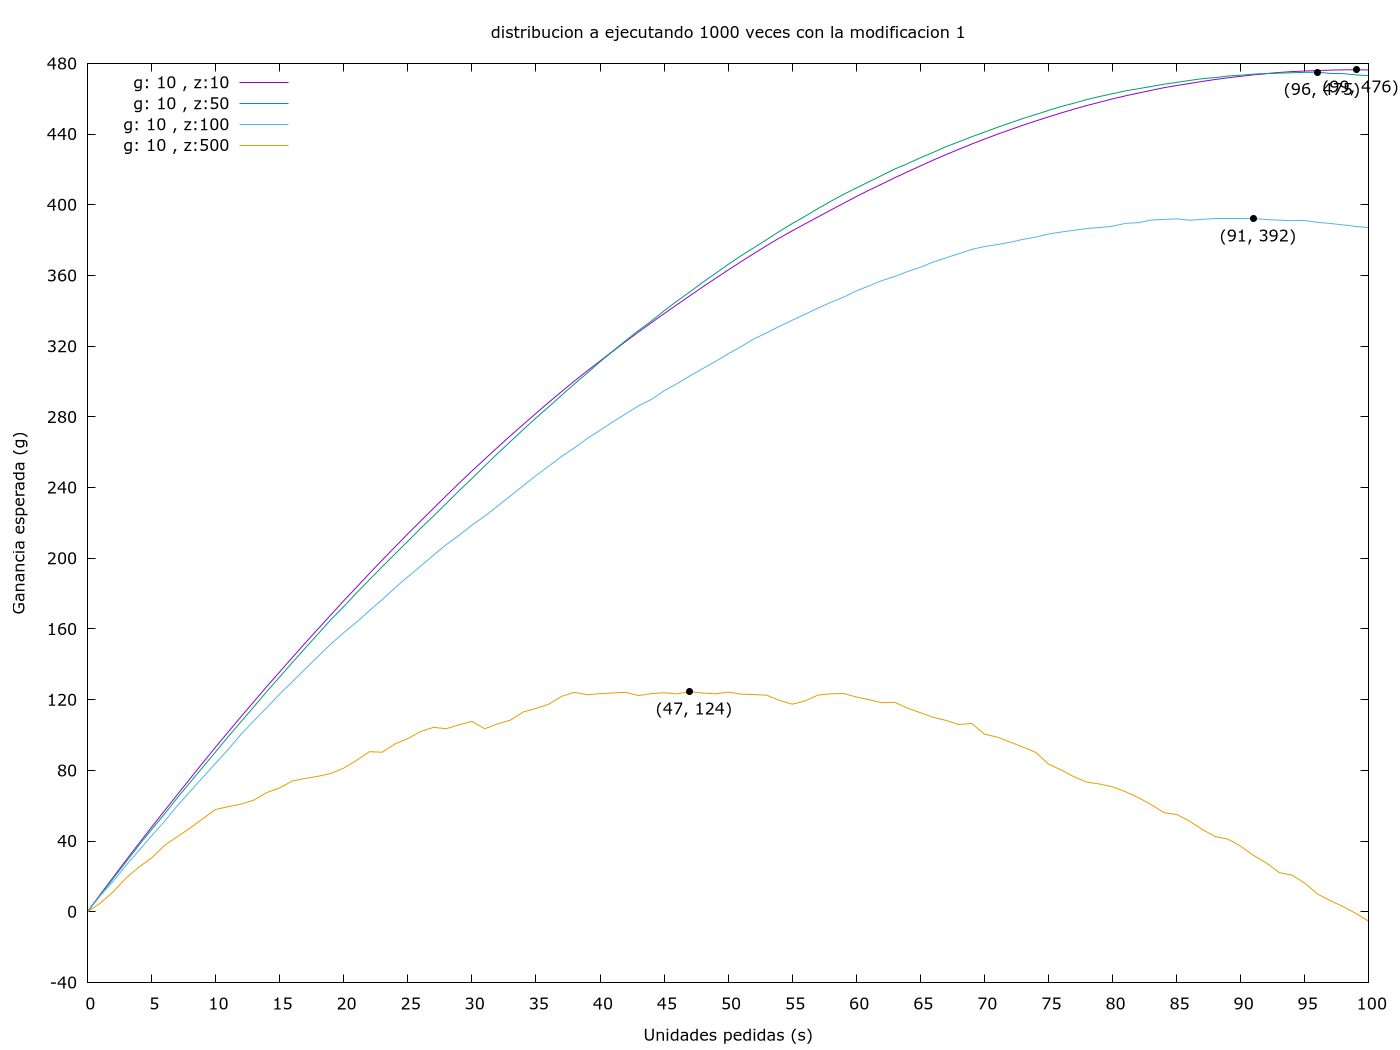
\includegraphics[scale = 0.2]{prob_a/datos_a_1000_1.png}
	\caption{Con 1000 repeticiones, la distribución a y la modificación 1.}
	\label{fig:ej1_a_1000}

\end{figure}

\begin{figure}[H]
	\centering
	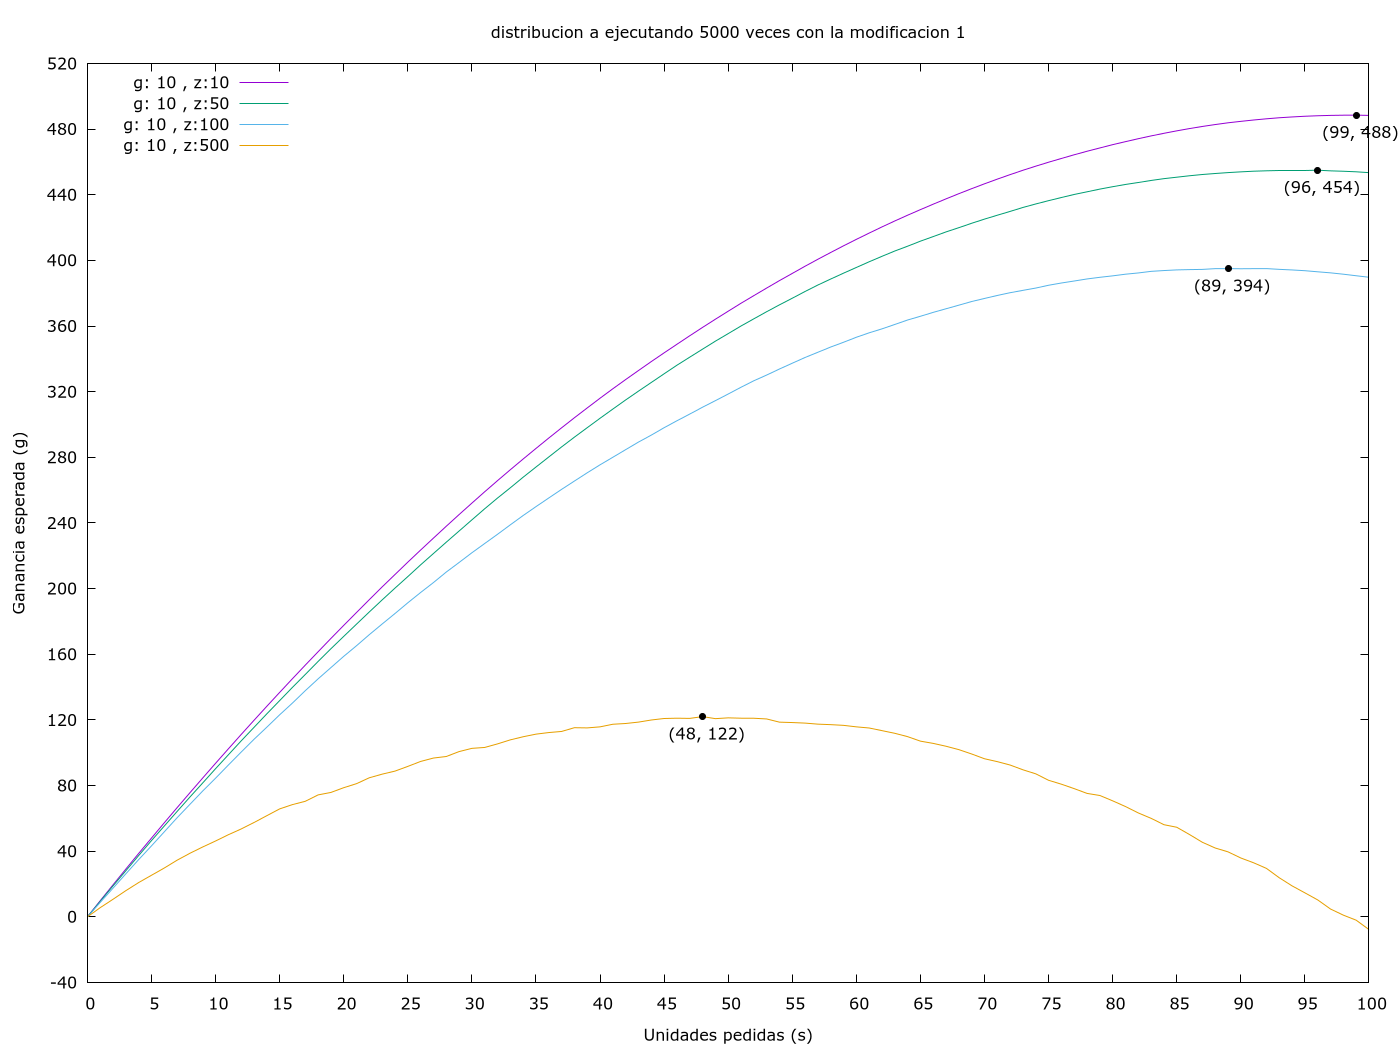
\includegraphics[scale = 0.2]{prob_a/datos_a_5000_1.png}
	\caption{Con 5000 repeticiones, la distribución a y la modificación 1.}
	\label{fig:ej1_a_5000}

\end{figure}


\begin{figure}[H]
	\centering
	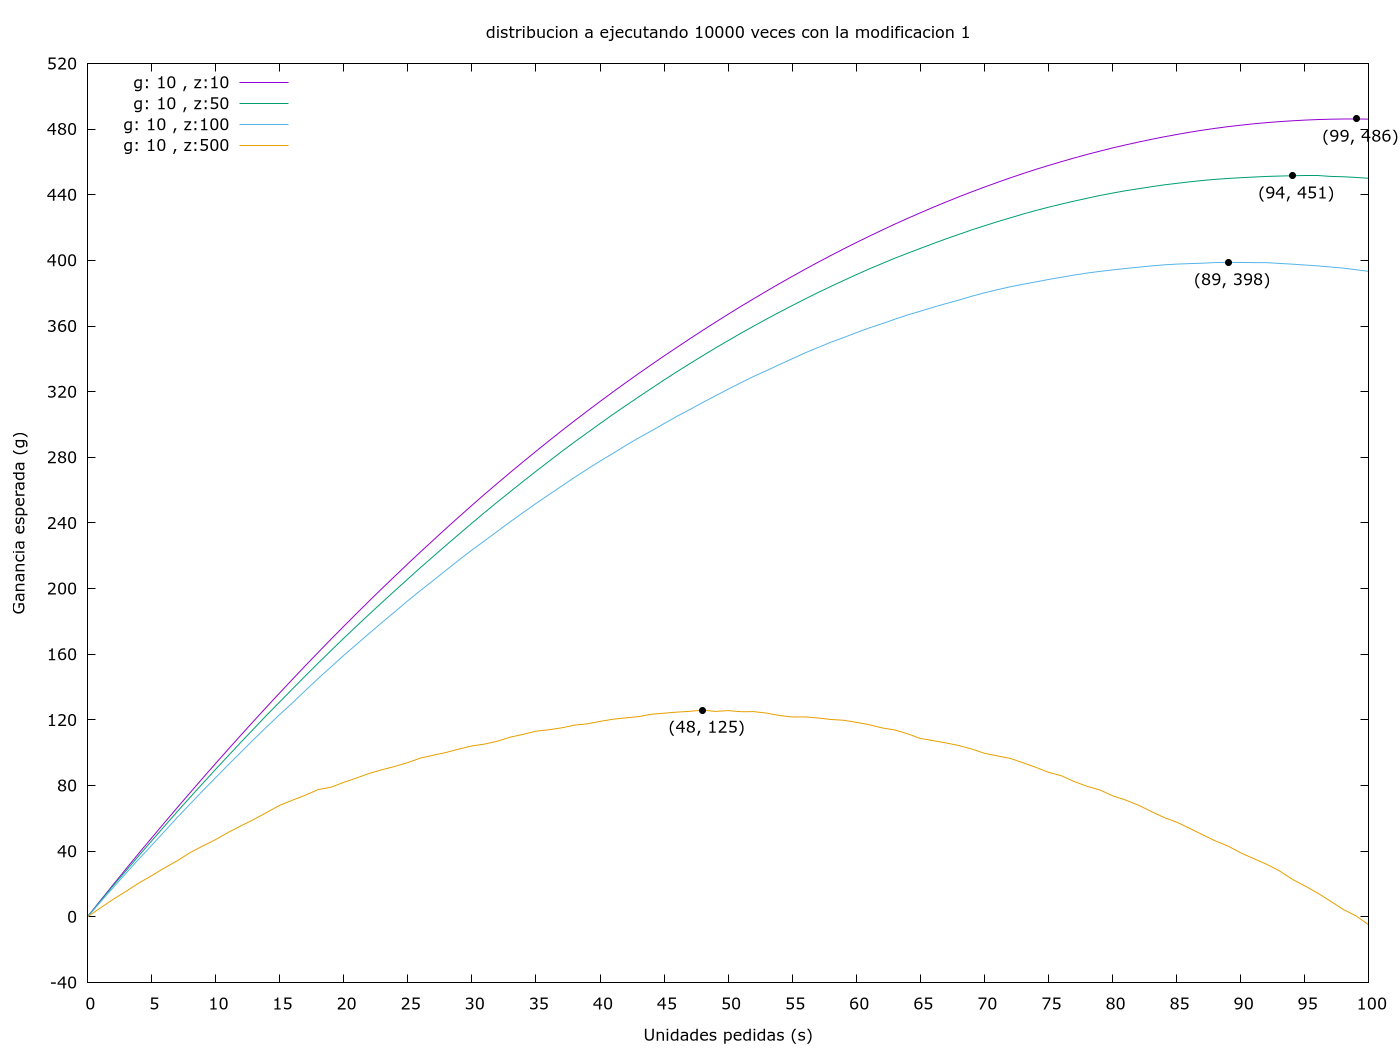
\includegraphics[scale = 0.2]{prob_a/datos_a_10000_1.png}
	\caption{Con 10000 repeticiones, la distribución a y la modificación 1.}
	\label{fig:ej1_a_10000}

\end{figure}

\begin{figure}[H]
	\centering
	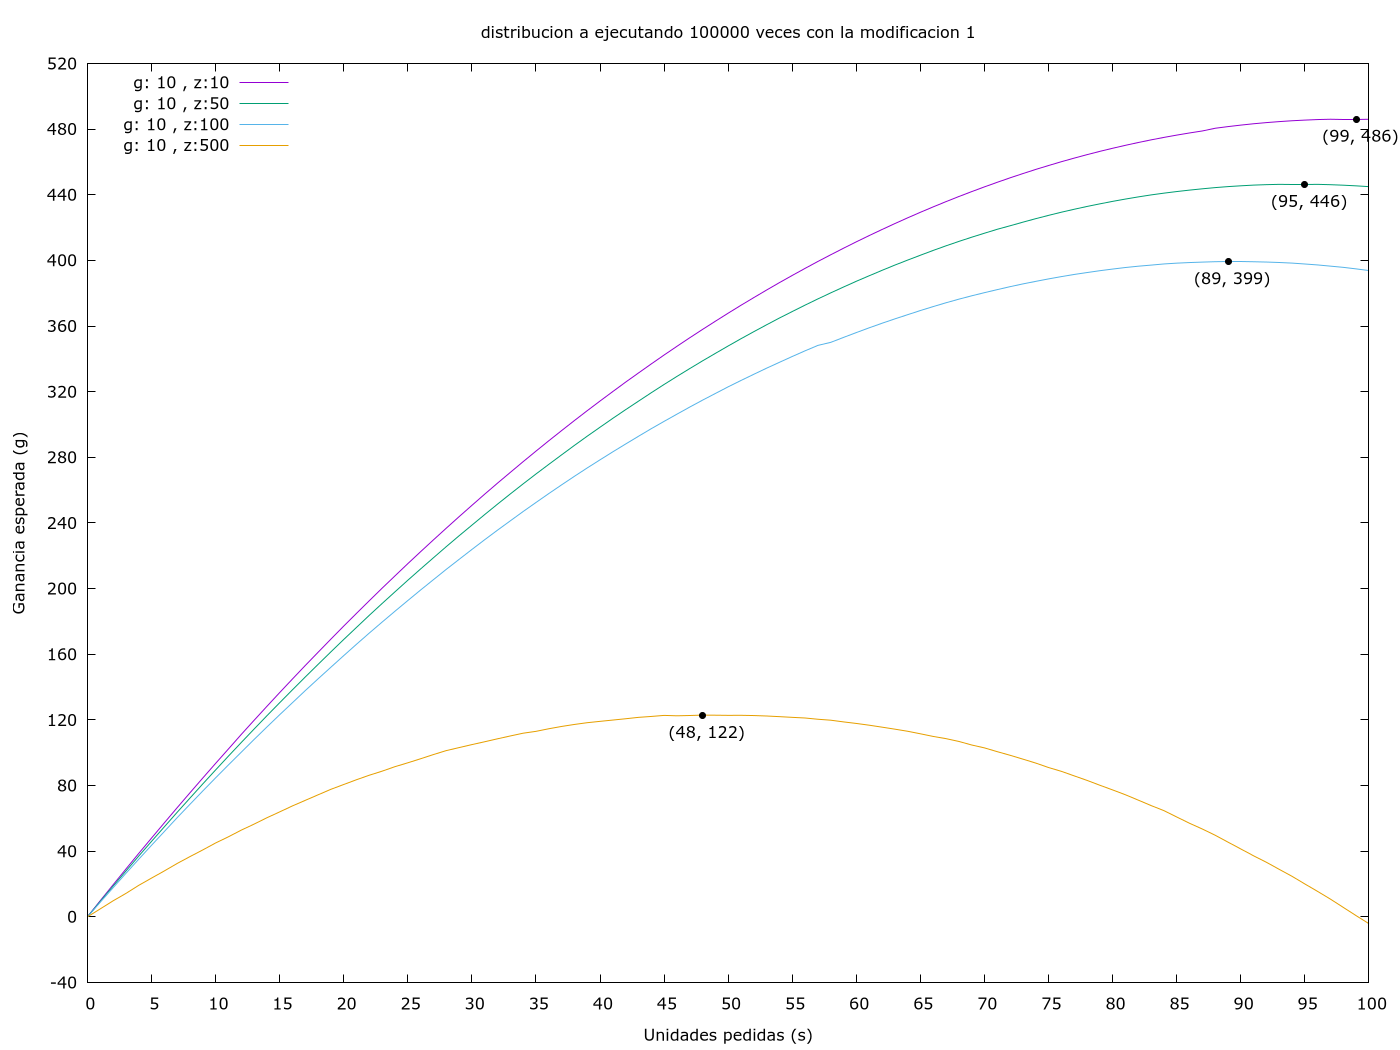
\includegraphics[scale = 0.2]{prob_a/datos_a_100000_1.png}
	\caption{Con 100000 repeticiones, la distribución a y la modificación 1.}
	\label{fig:ej1_a_100000}

\end{figure}

\begin{figure}[H]
	\centering
	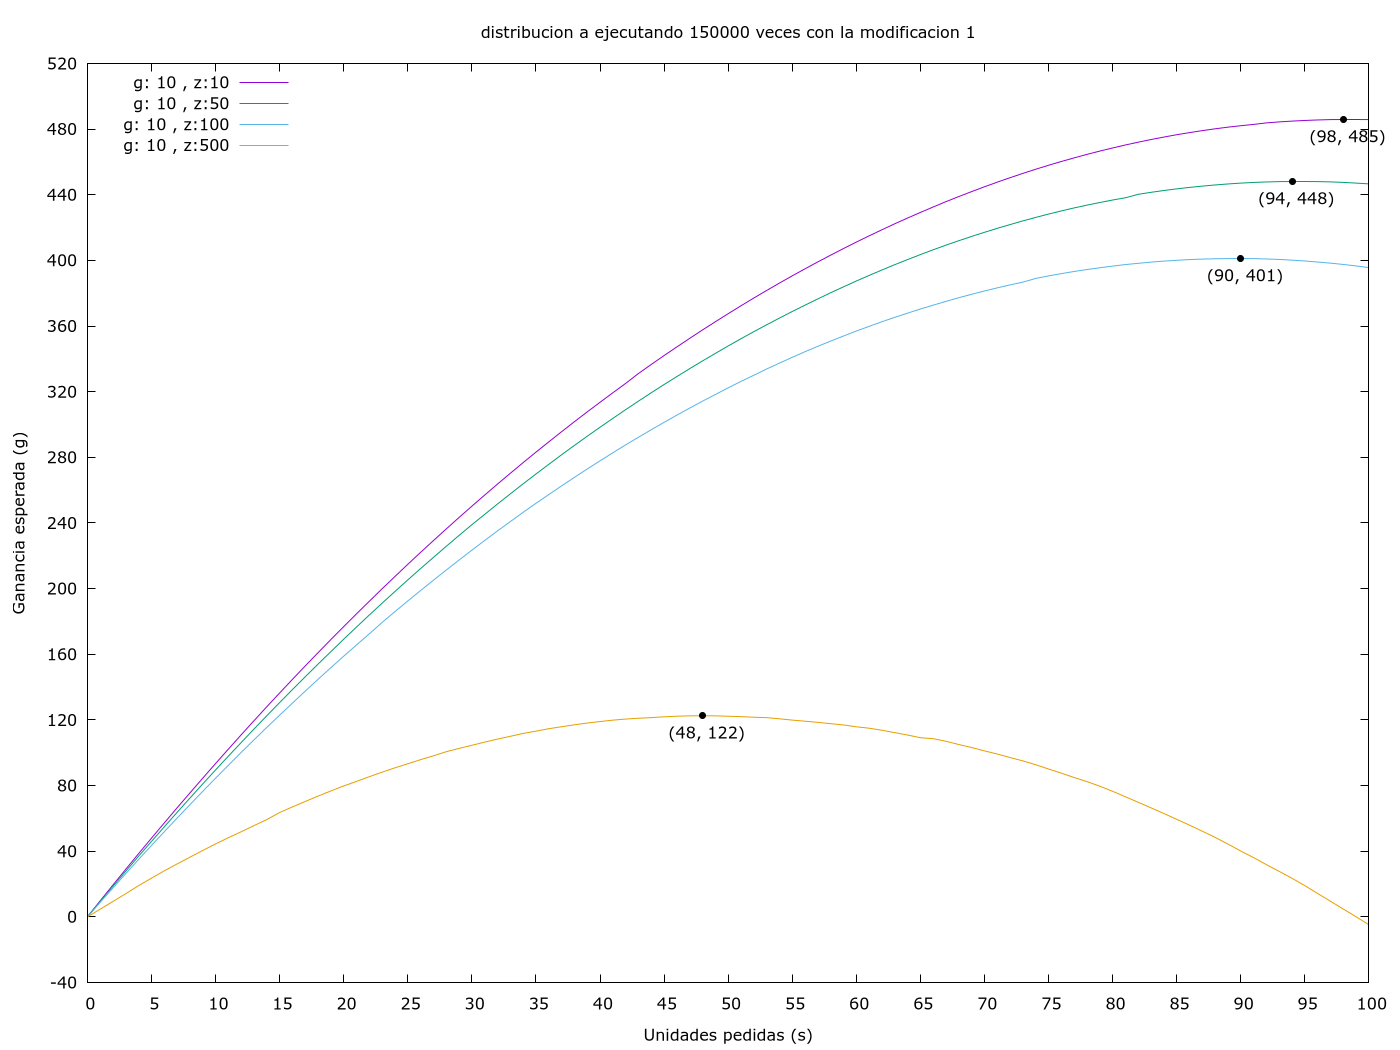
\includegraphics[scale = 0.2]{prob_a/datos_a_150000_1.png}
	\caption{Con 150000 repeticiones, la distribución a y la modificación 1.}
	\label{fig:ej1_a_150000}

\end{figure}



\subsubsection{Resultados obtenidos con la distribución b}



\begin{figure}[H]
	\centering
	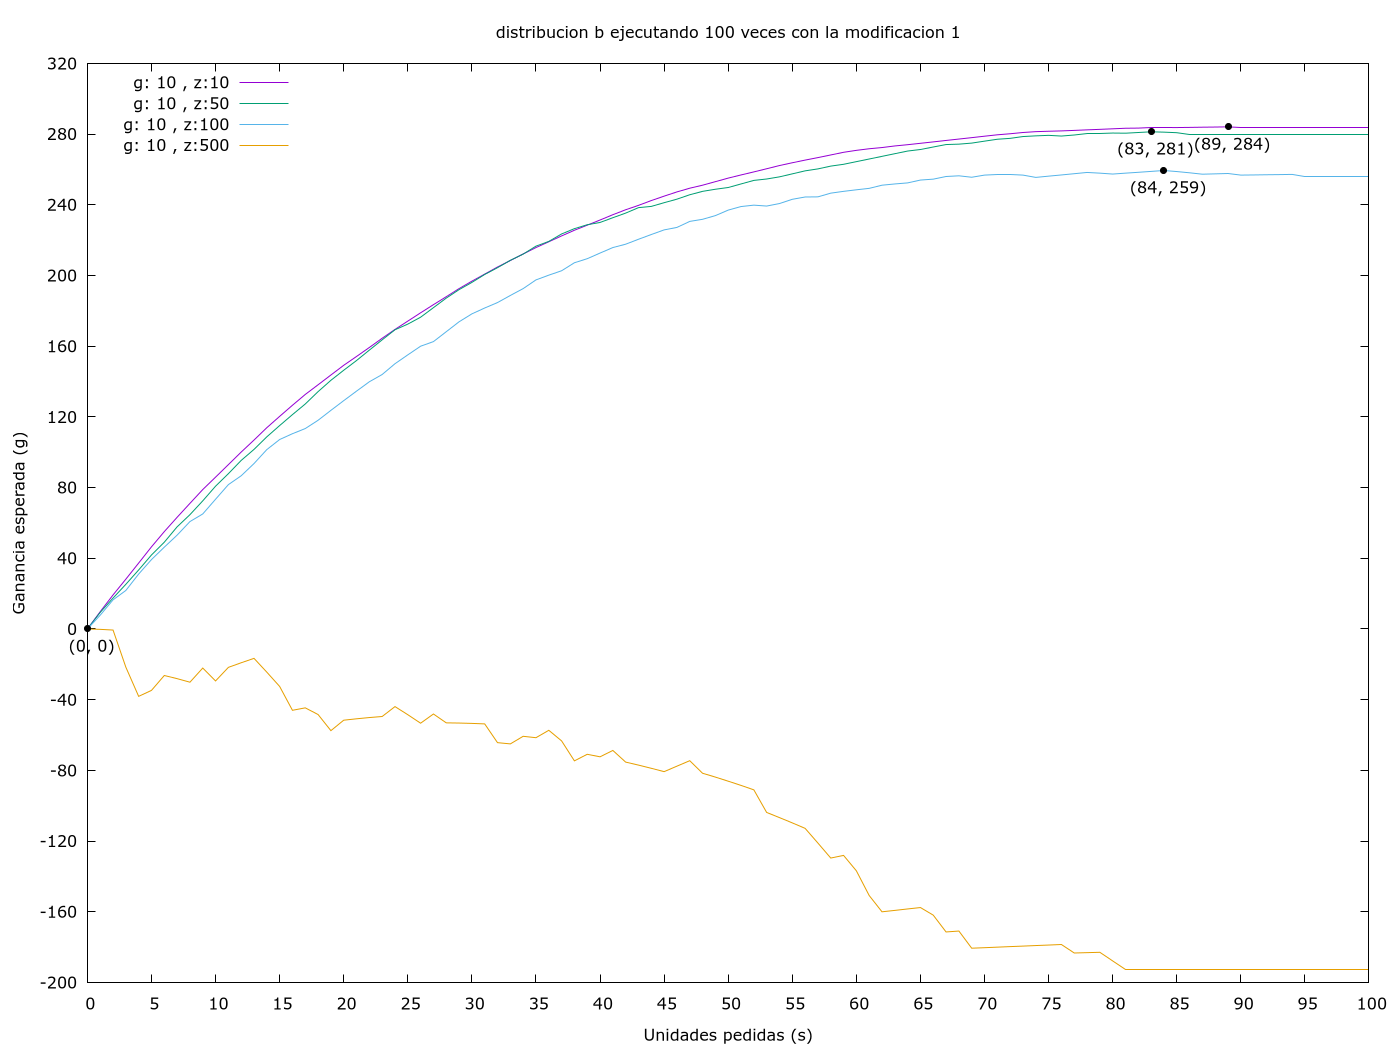
\includegraphics[scale = 0.2]{prob_b/datos_b_100_1.png}
	\caption{Con 100 repeticiones, la distribución b y la modificación 1.}
	\label{fig:ej1_a_100}

\end{figure}

\begin{figure}[H]
	\centering
	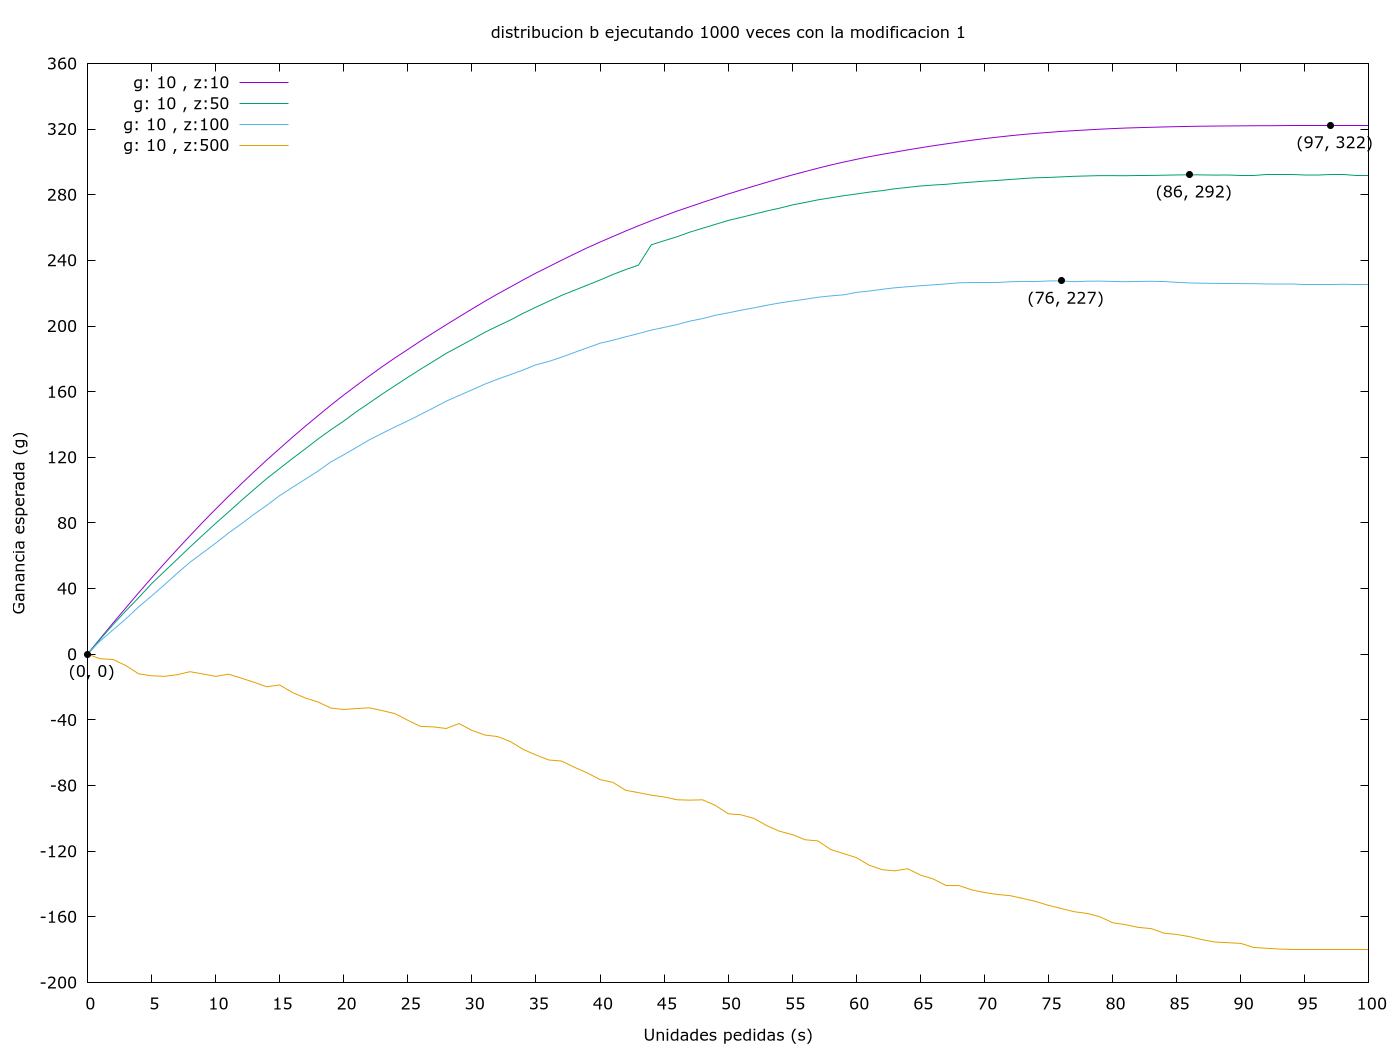
\includegraphics[scale = 0.2]{prob_b/datos_b_1000_1.png}
	\caption{Con 1000 repeticiones, la distribución b y la modificación 1.}
	\label{fig:ej1_a_1000}

\end{figure}

\begin{figure}[H]
	\centering
	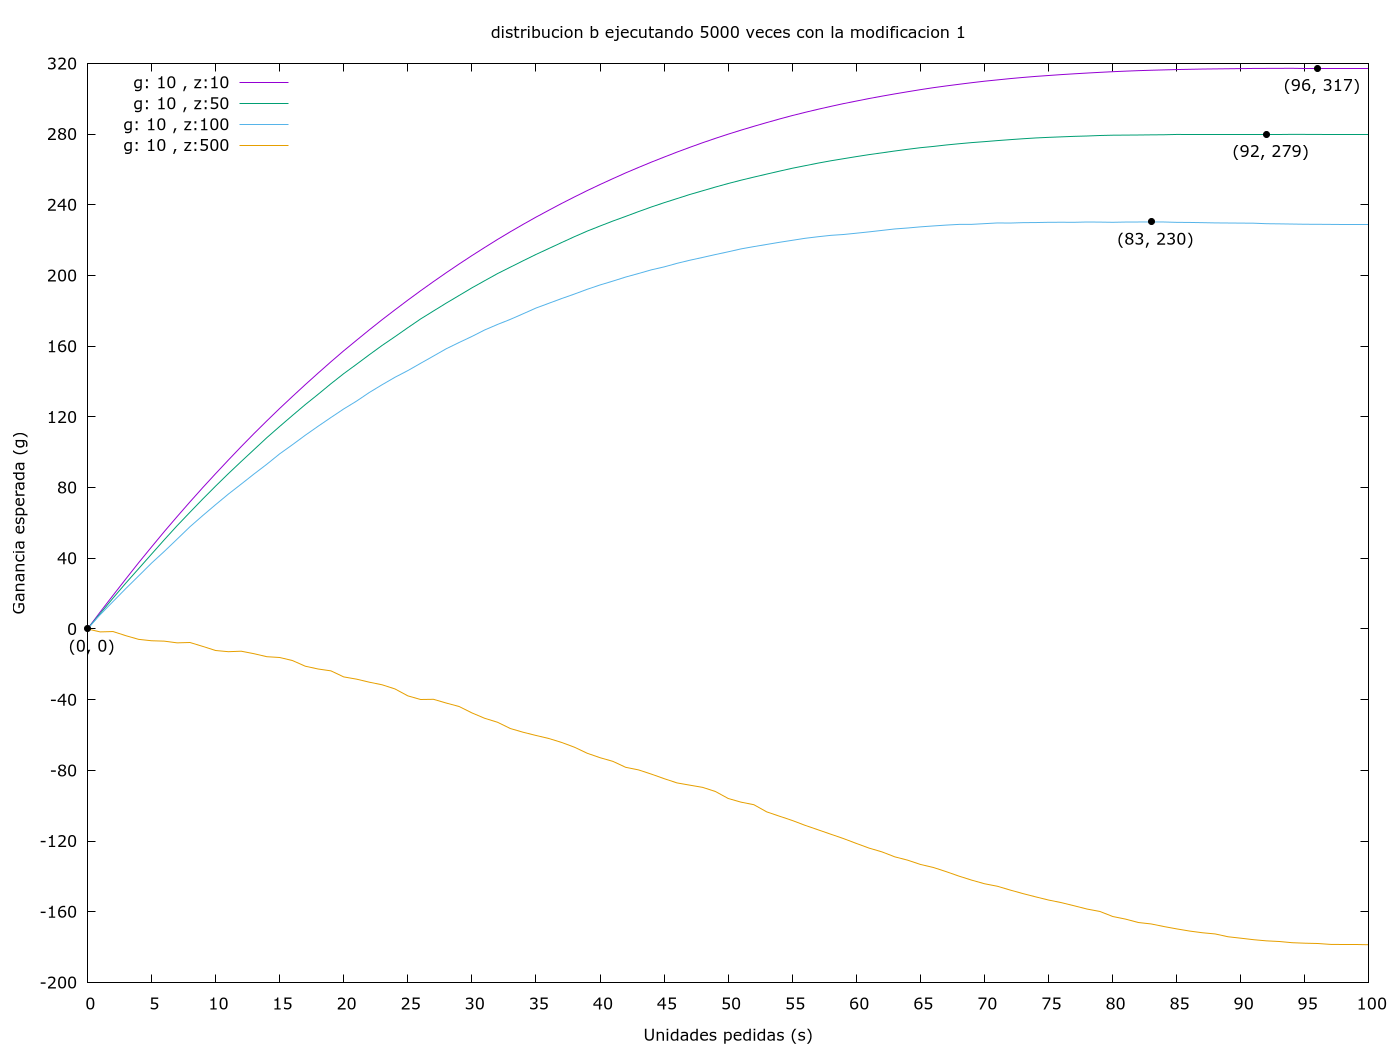
\includegraphics[scale = 0.2]{prob_b/datos_b_5000_1.png}
	\caption{Con 5000 repeticiones, la distribución b y la modificación 1.}
	\label{fig:ej1_a_5000}

\end{figure}


\begin{figure}[H]
	\centering
	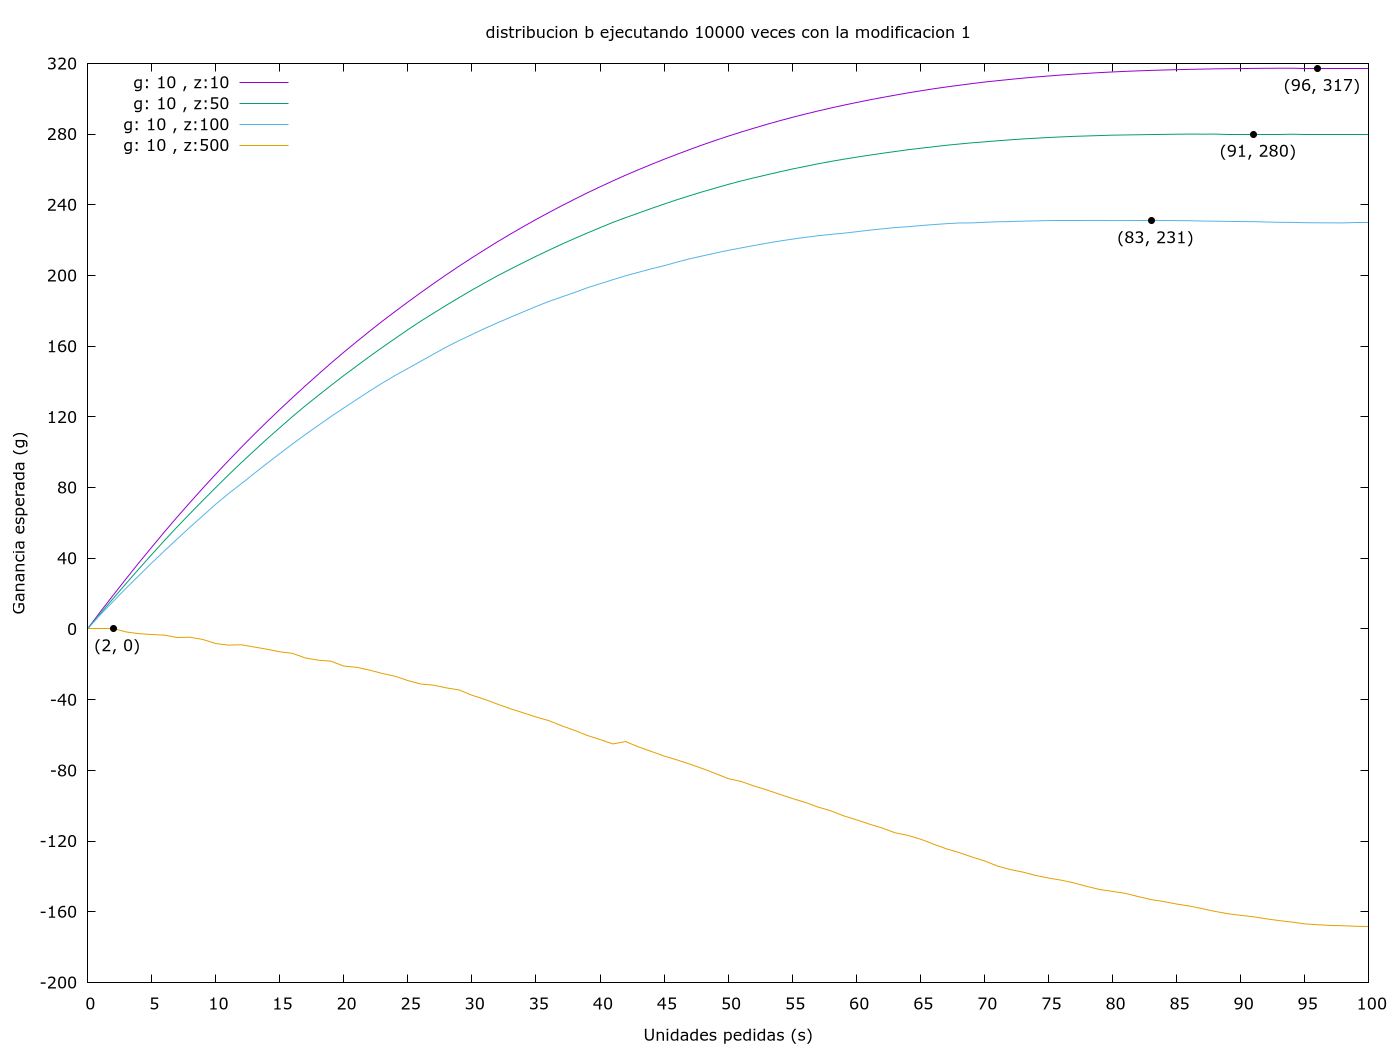
\includegraphics[scale = 0.2]{prob_b/datos_b_10000_1.png}
	\caption{Con 10000 repeticiones, la distribución b y la modificación 1.}
	\label{fig:ej1_a_10000}

\end{figure}

\begin{figure}[H]
	\centering
	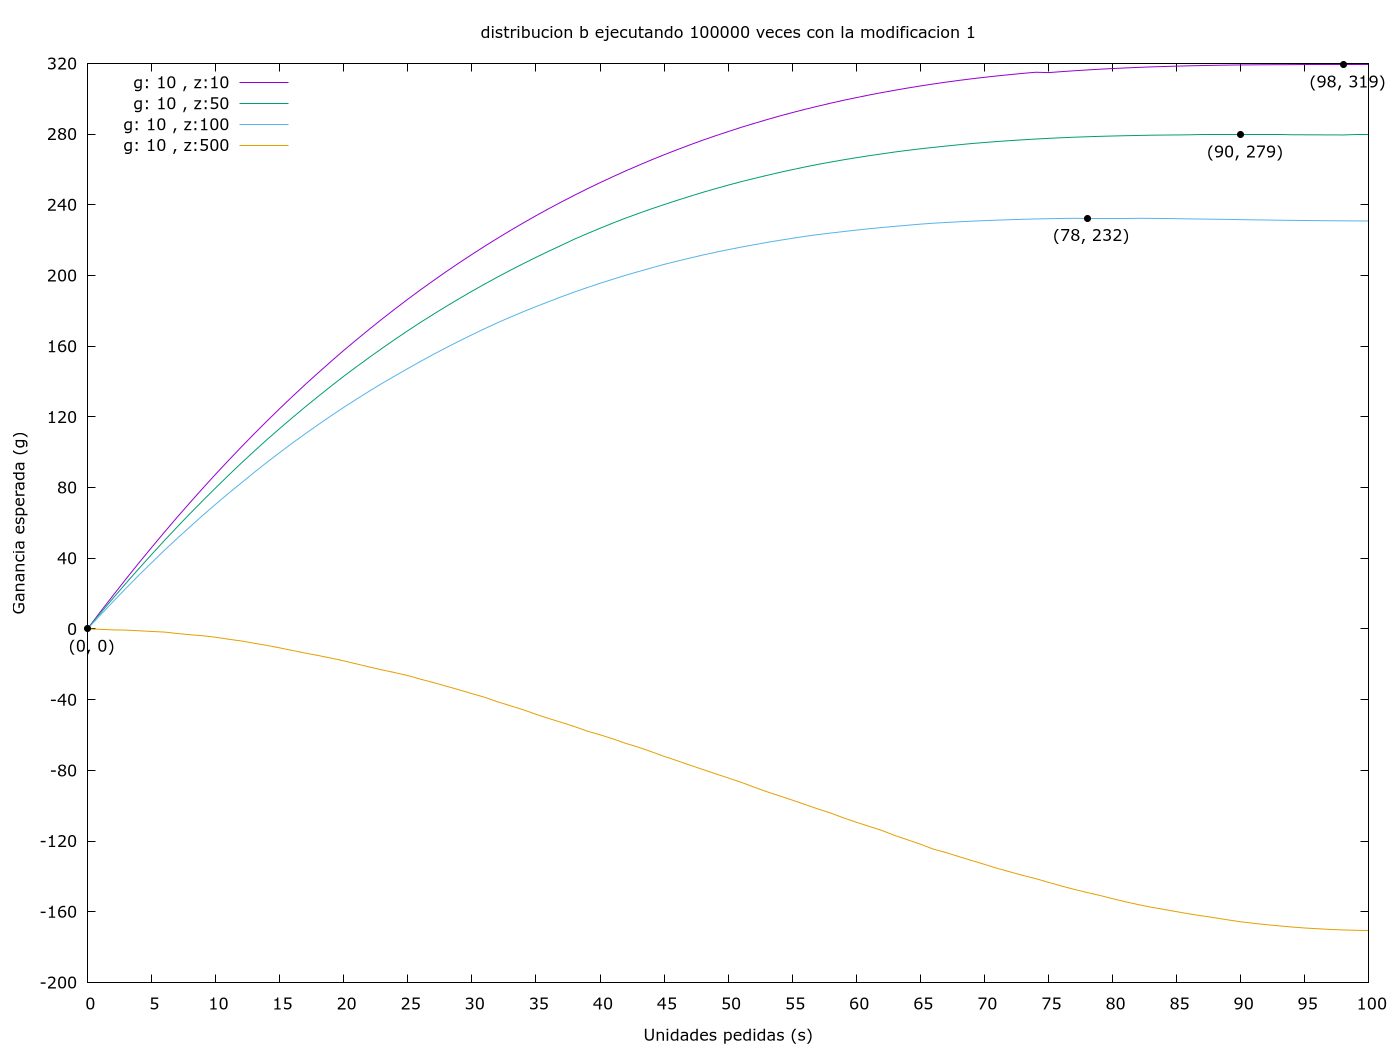
\includegraphics[scale = 0.2]{prob_b/datos_b_100000_1.png}
	\caption{Con 100000 repeticiones, la distribución b y la modificación 1.}
	\label{fig:ej1_a_100000}

\end{figure}

\begin{figure}[H]
	\centering
	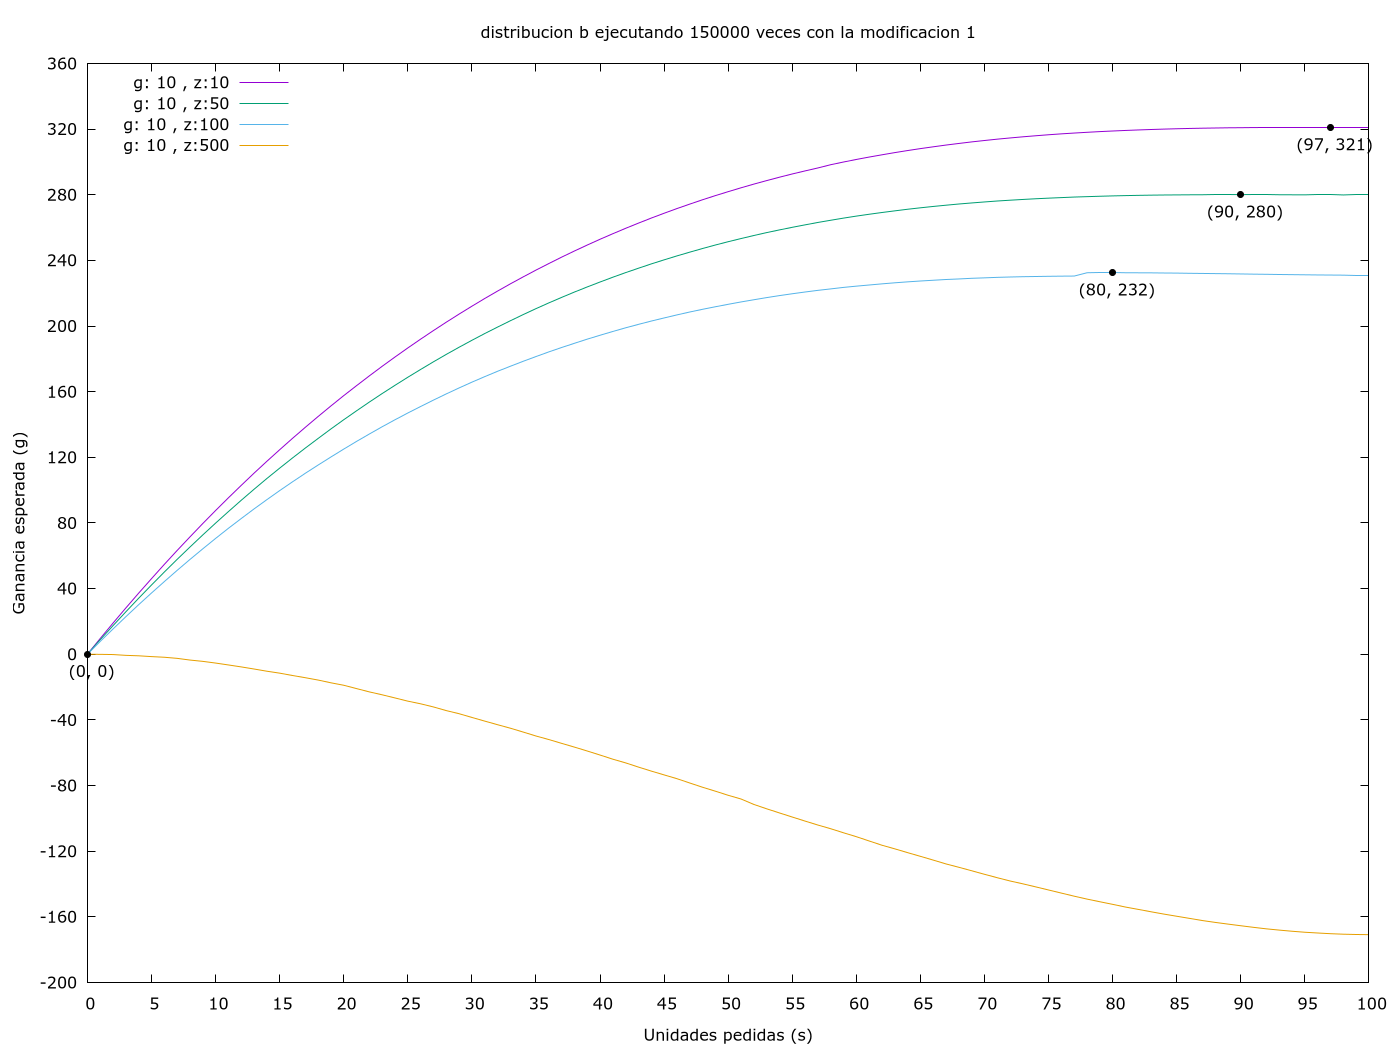
\includegraphics[scale = 0.2]{prob_b/datos_b_150000_1.png}
	\caption{Con 150000 repeticiones, la distribución b y la modificación 1.}
	\label{fig:ej1_a_150000}

\end{figure}

\subsubsection{Resultados obtenidos con la distribución c}



\begin{figure}[H]
	\centering
	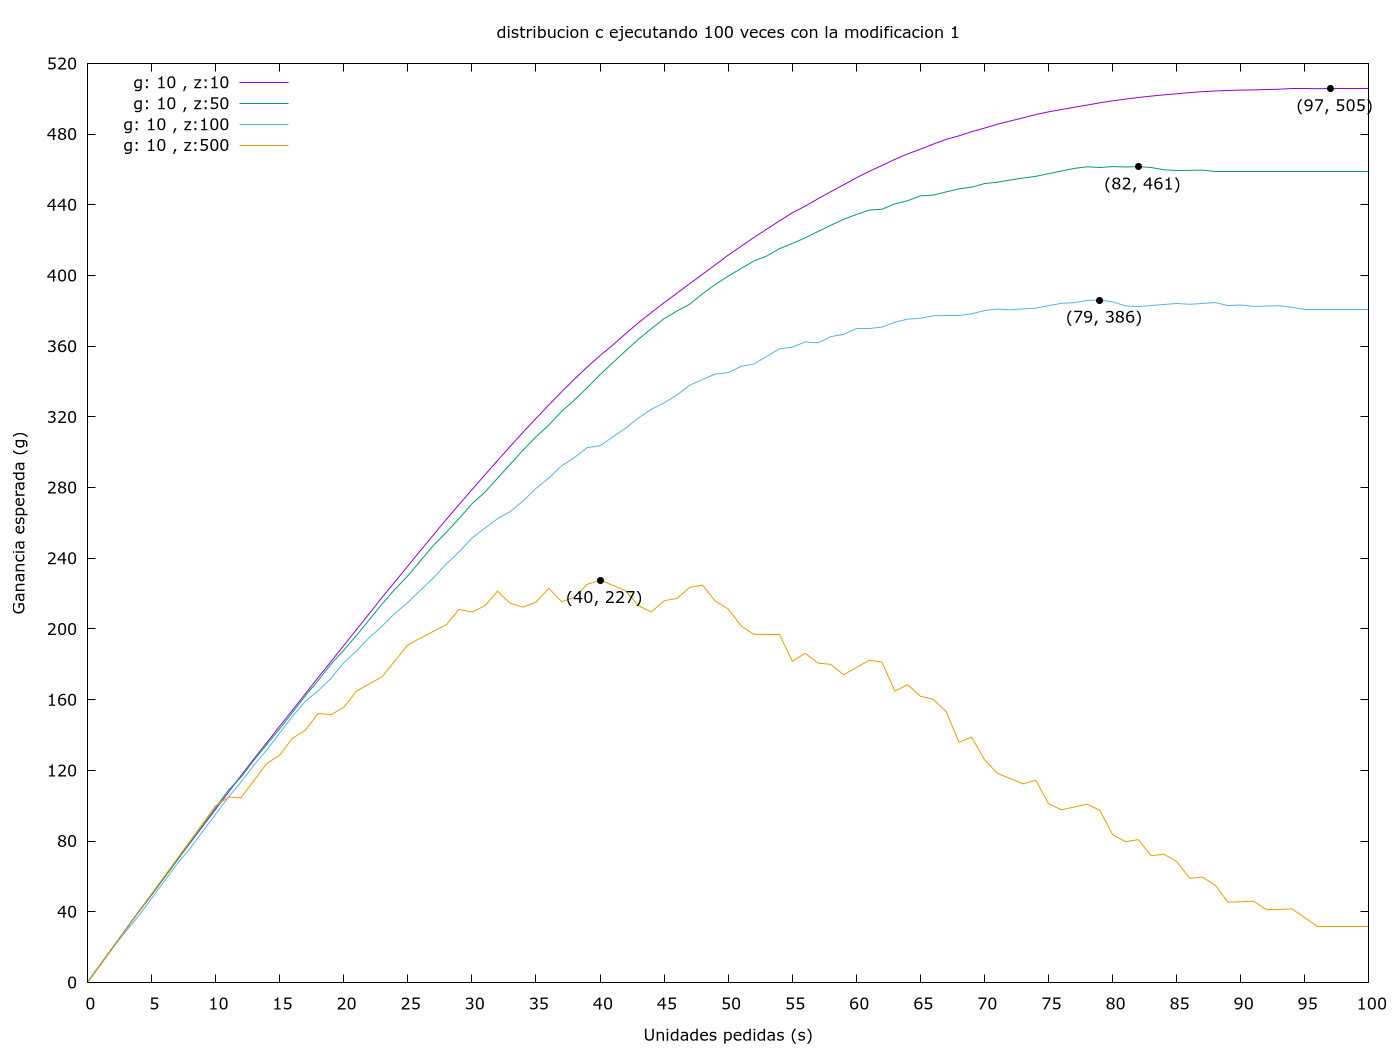
\includegraphics[scale = 0.2]{prob_c/datos_c_100_1.png}
	\caption{Con 100 repeticiones, la distribución b y la modificación 1.}
	\label{fig:ej1_a_100}

\end{figure}

\begin{figure}[H]
	\centering
	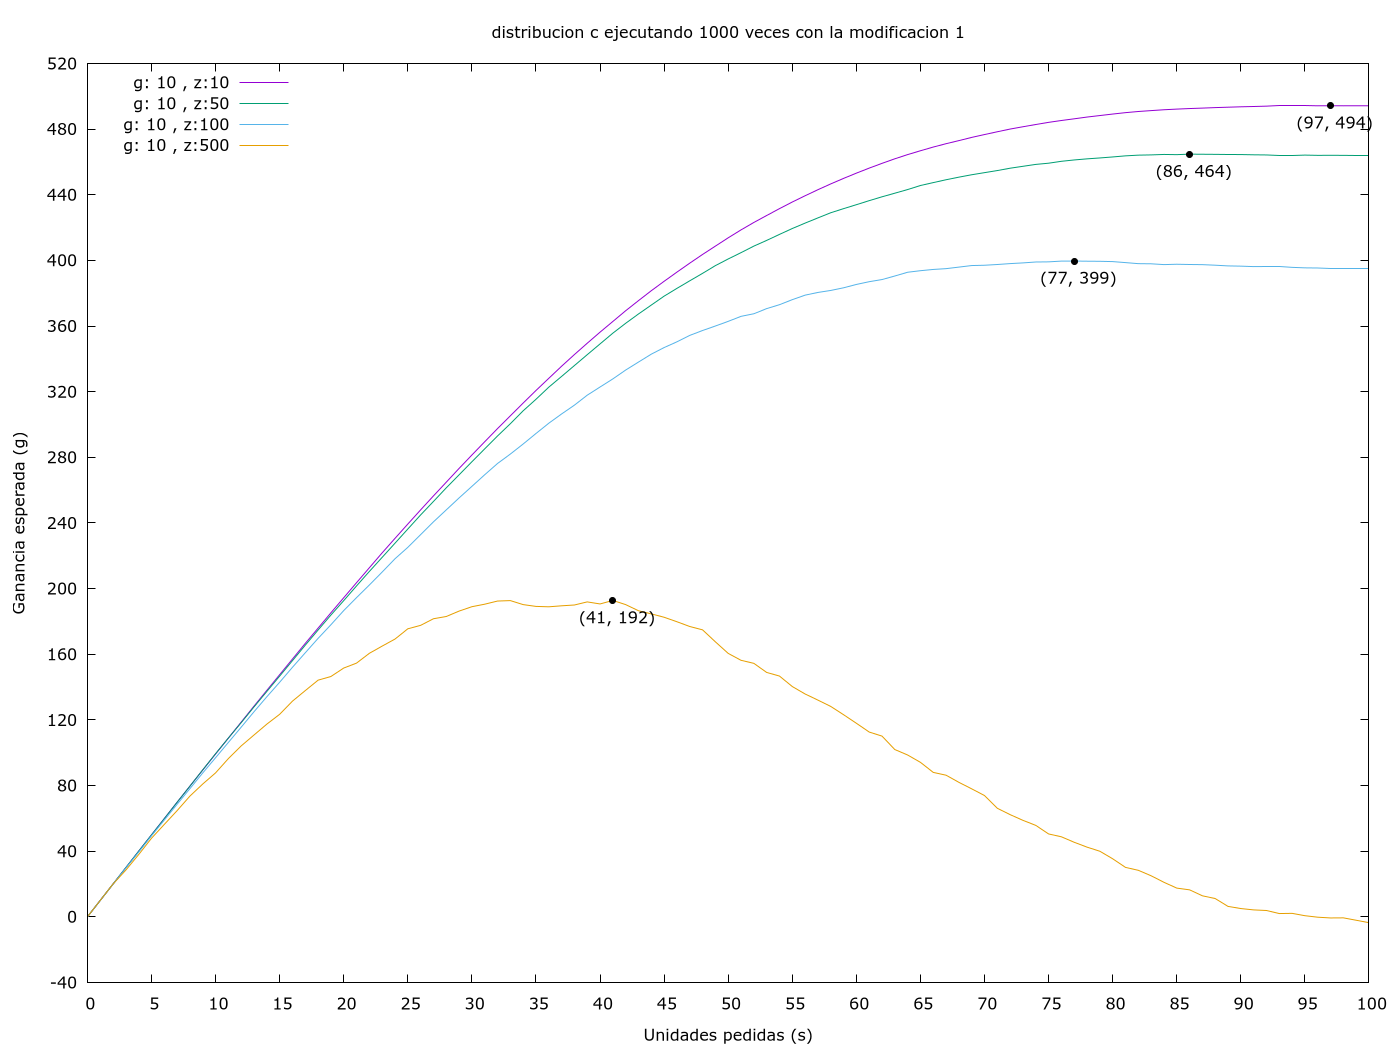
\includegraphics[scale = 0.2]{prob_c/datos_c_1000_1.png}
	\caption{Con 1000 repeticiones, la distribución b y la modificación 1.}
	\label{fig:ej1_a_1000}

\end{figure}

\begin{figure}[H]
	\centering
	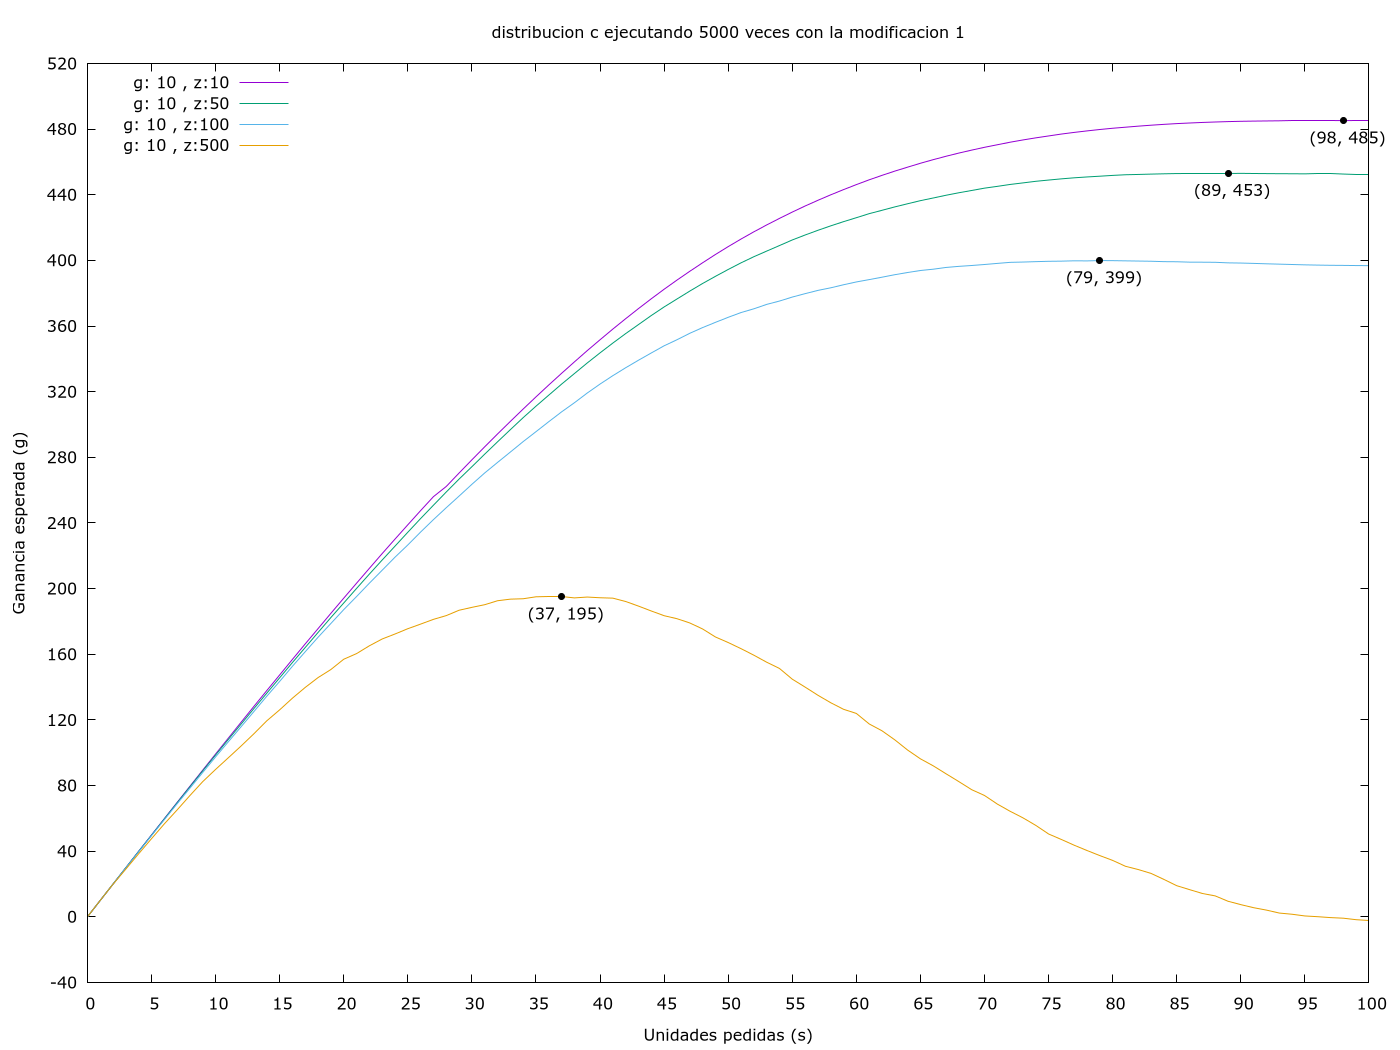
\includegraphics[scale = 0.2]{prob_c/datos_c_5000_1.png}
	\caption{Con 5000 repeticiones, la distribución b y la modificación 1.}
	\label{fig:ej1_a_5000}

\end{figure}


\begin{figure}[H]
	\centering
	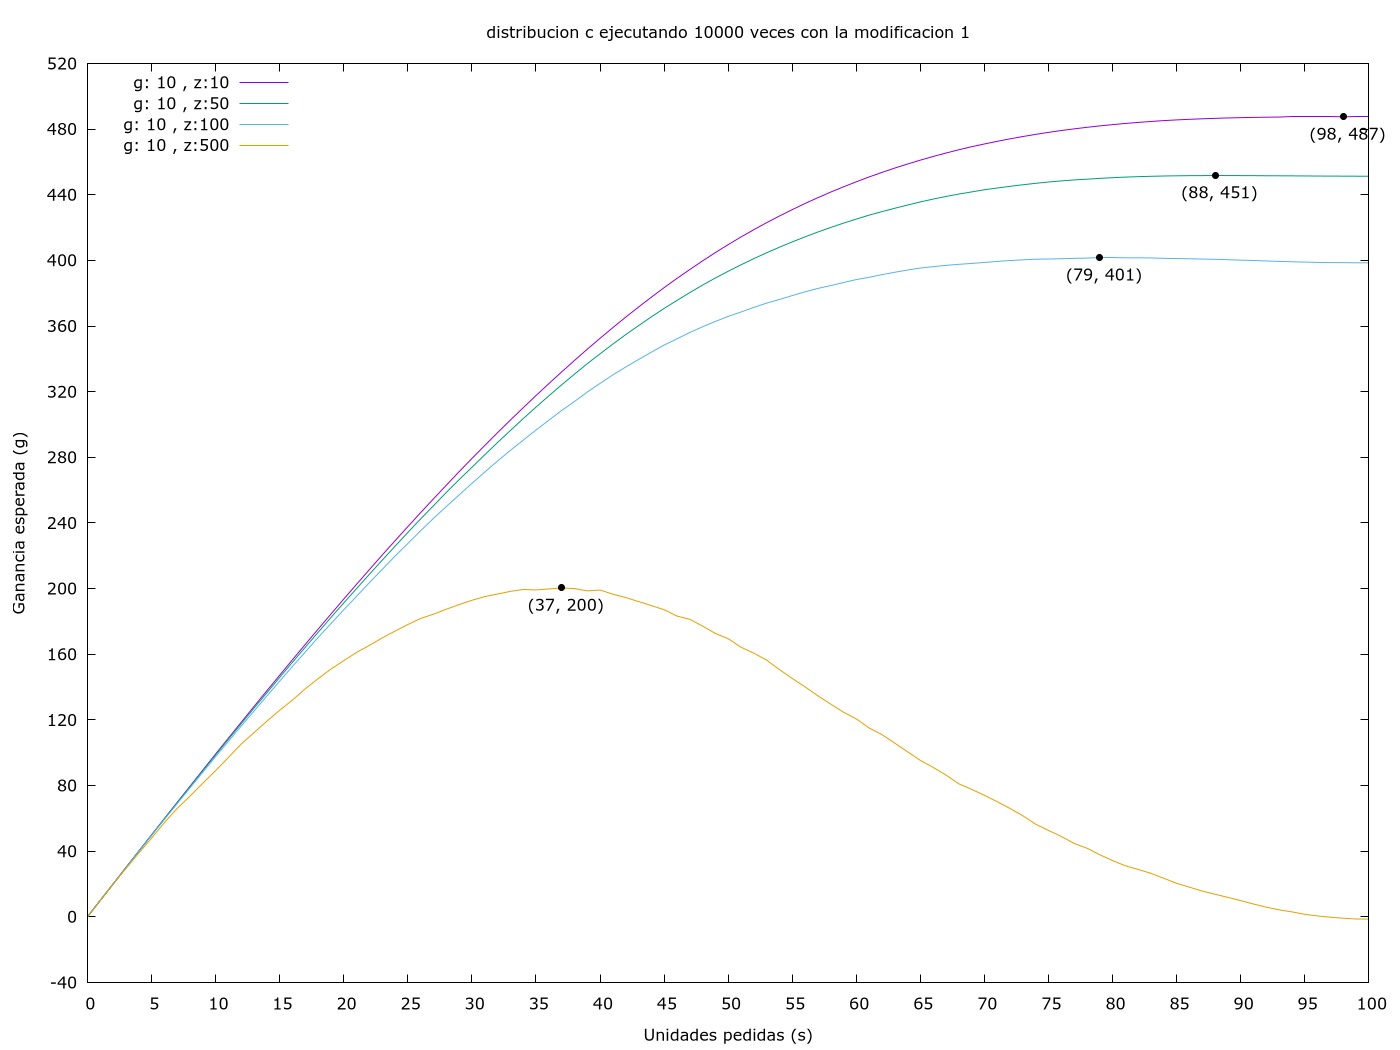
\includegraphics[scale = 0.2]{prob_c/datos_c_10000_1.png}
	\caption{Con 10000 repeticiones, la distribución b y la modificación 1.}
	\label{fig:ej1_a_10000}

\end{figure}

\begin{figure}[H]
	\centering
	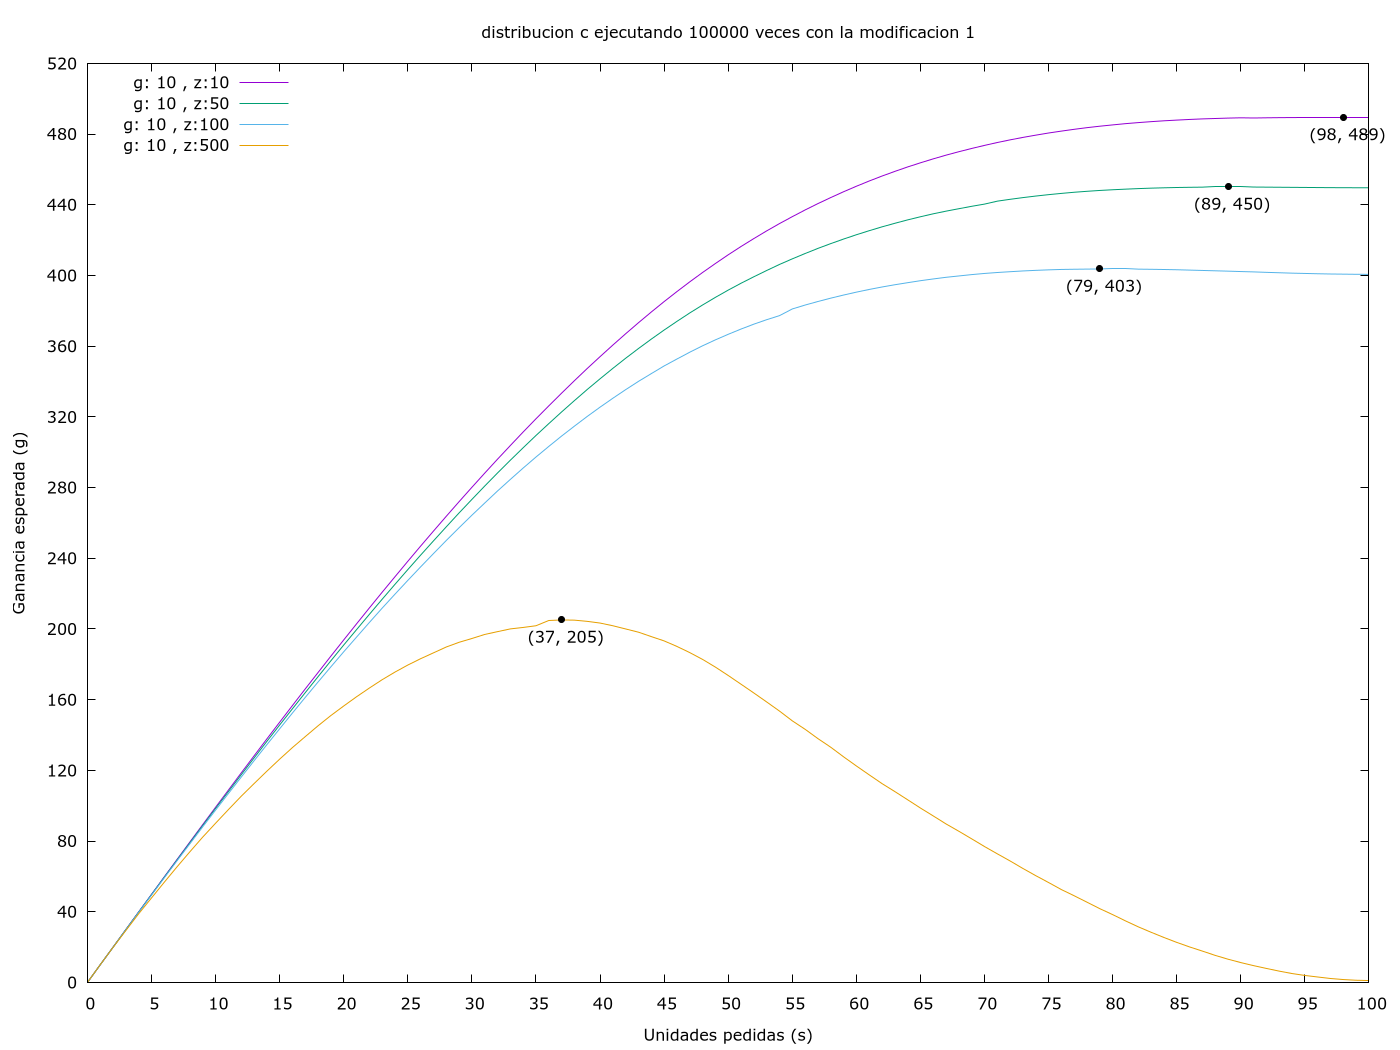
\includegraphics[scale = 0.2]{prob_c/datos_c_100000_1.png}
	\caption{Con 100000 repeticiones, la distribución b y la modificación 1.}
	\label{fig:ej1_a_100000}

\end{figure}

\begin{figure}[H]
	\centering
	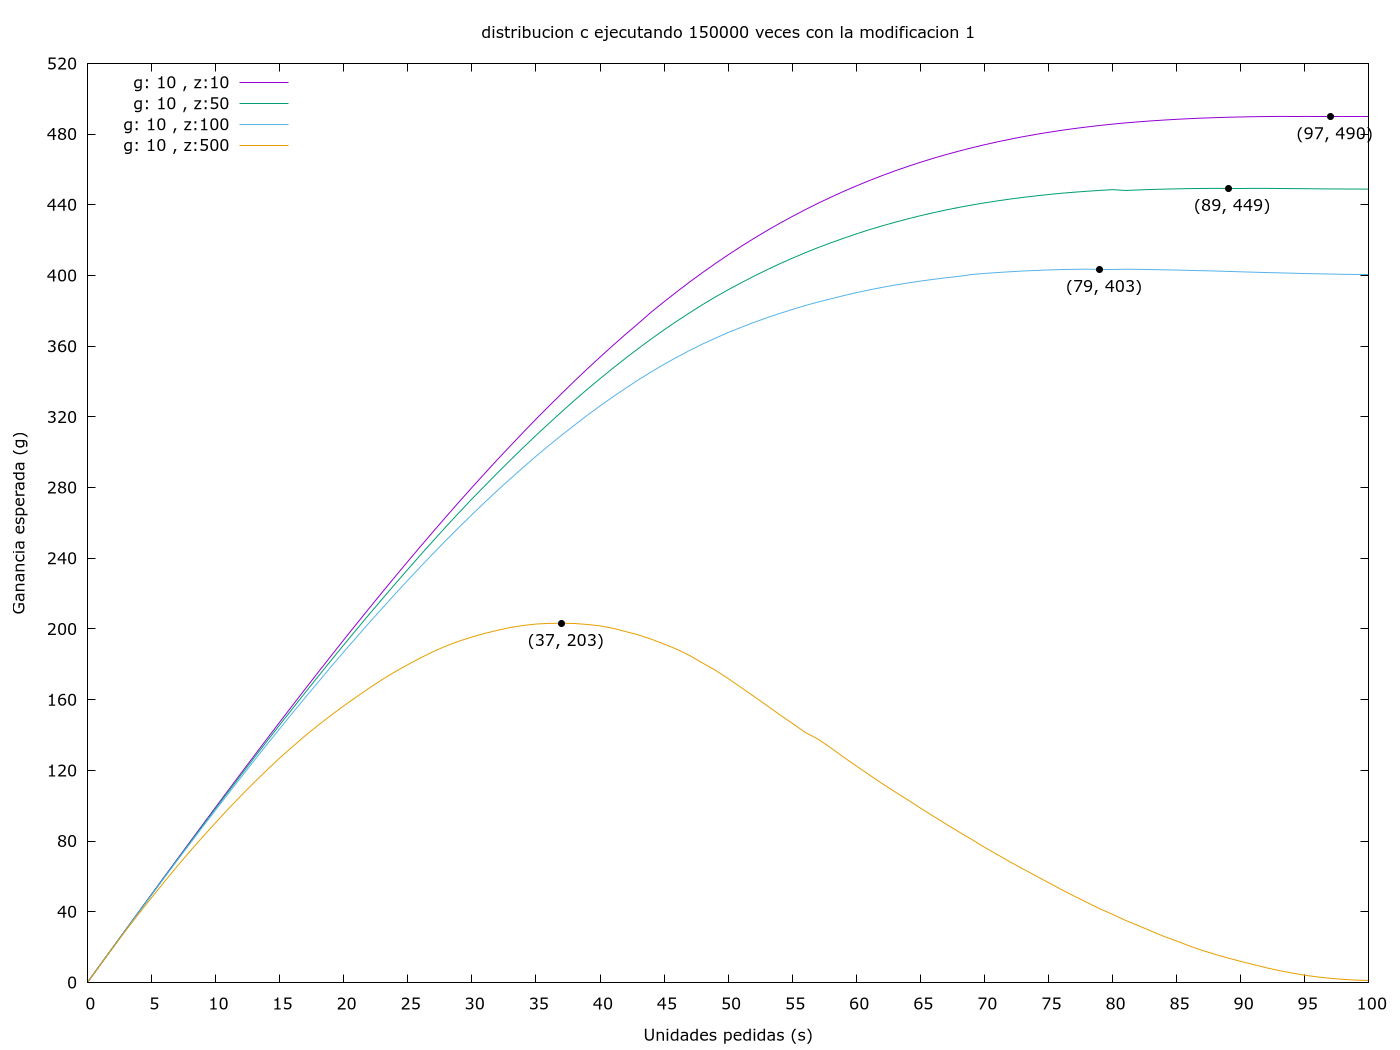
\includegraphics[scale = 0.2]{prob_c/datos_c_150000_1.png}
	\caption{Con 150000 repeticiones, la distribución b y la modificación 1.}
	\label{fig:ej1_a_150000}

\end{figure}

\subsection{Modificación 2 del modelo}

\subsubsection{Resultados obtenidos con la distribución a}


\begin{figure}[H]
	\centering
	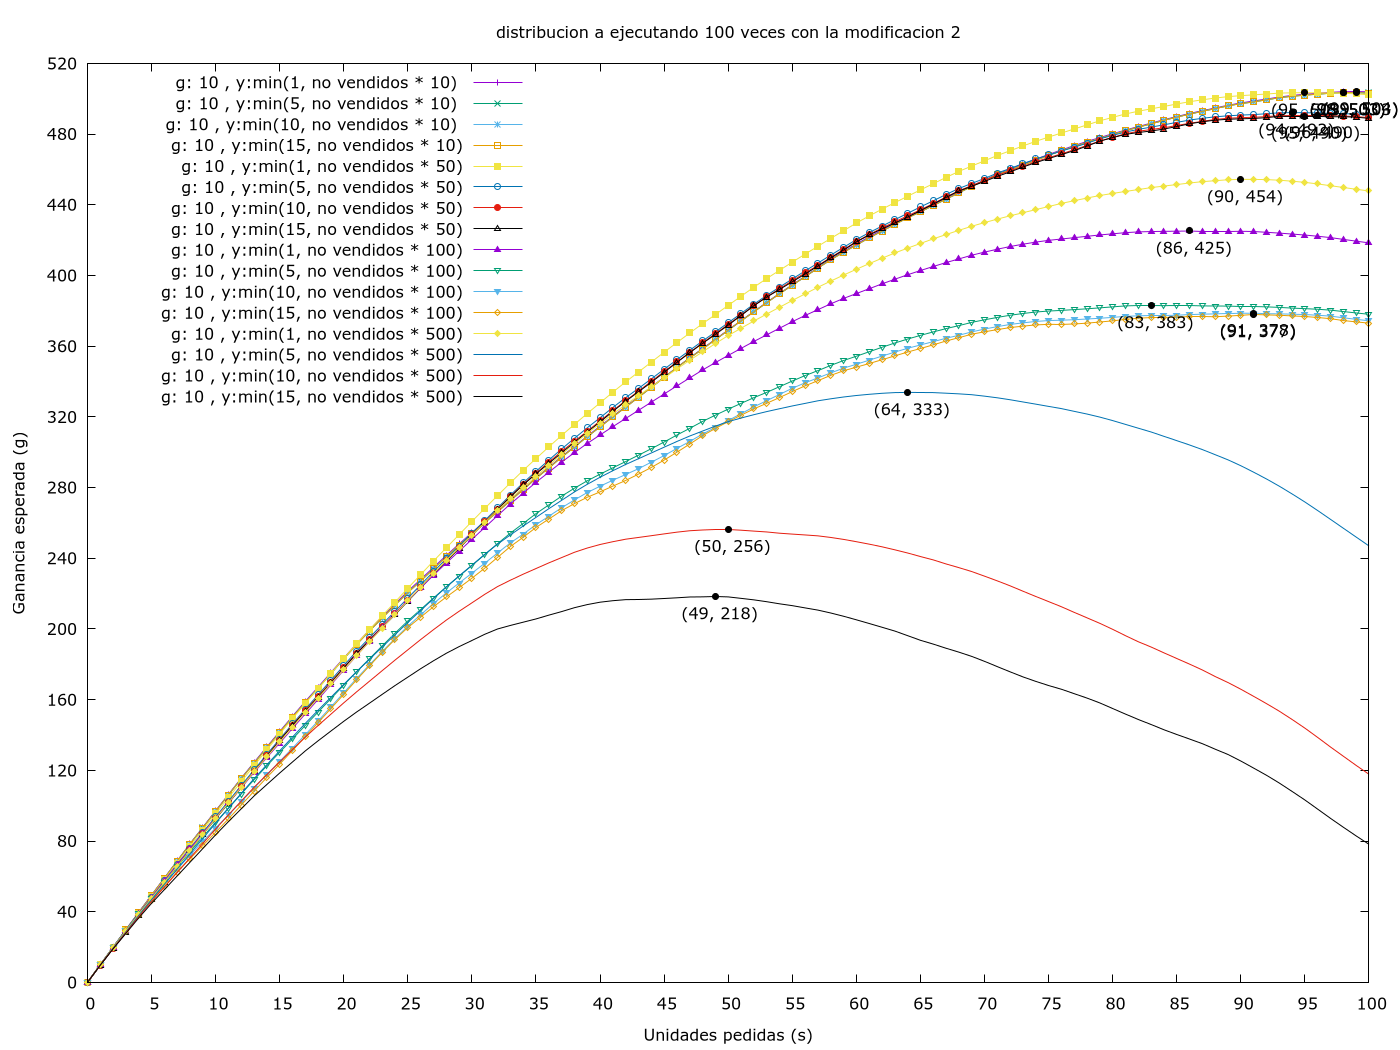
\includegraphics[scale = 0.2]{prob_a/datos_a_100_2.png}
	\caption{Con 100 repeticiones, la distribución a y la modificación 2.}
	\label{fig:ej1_a_100}

\end{figure}

\begin{figure}[H]
	\centering
	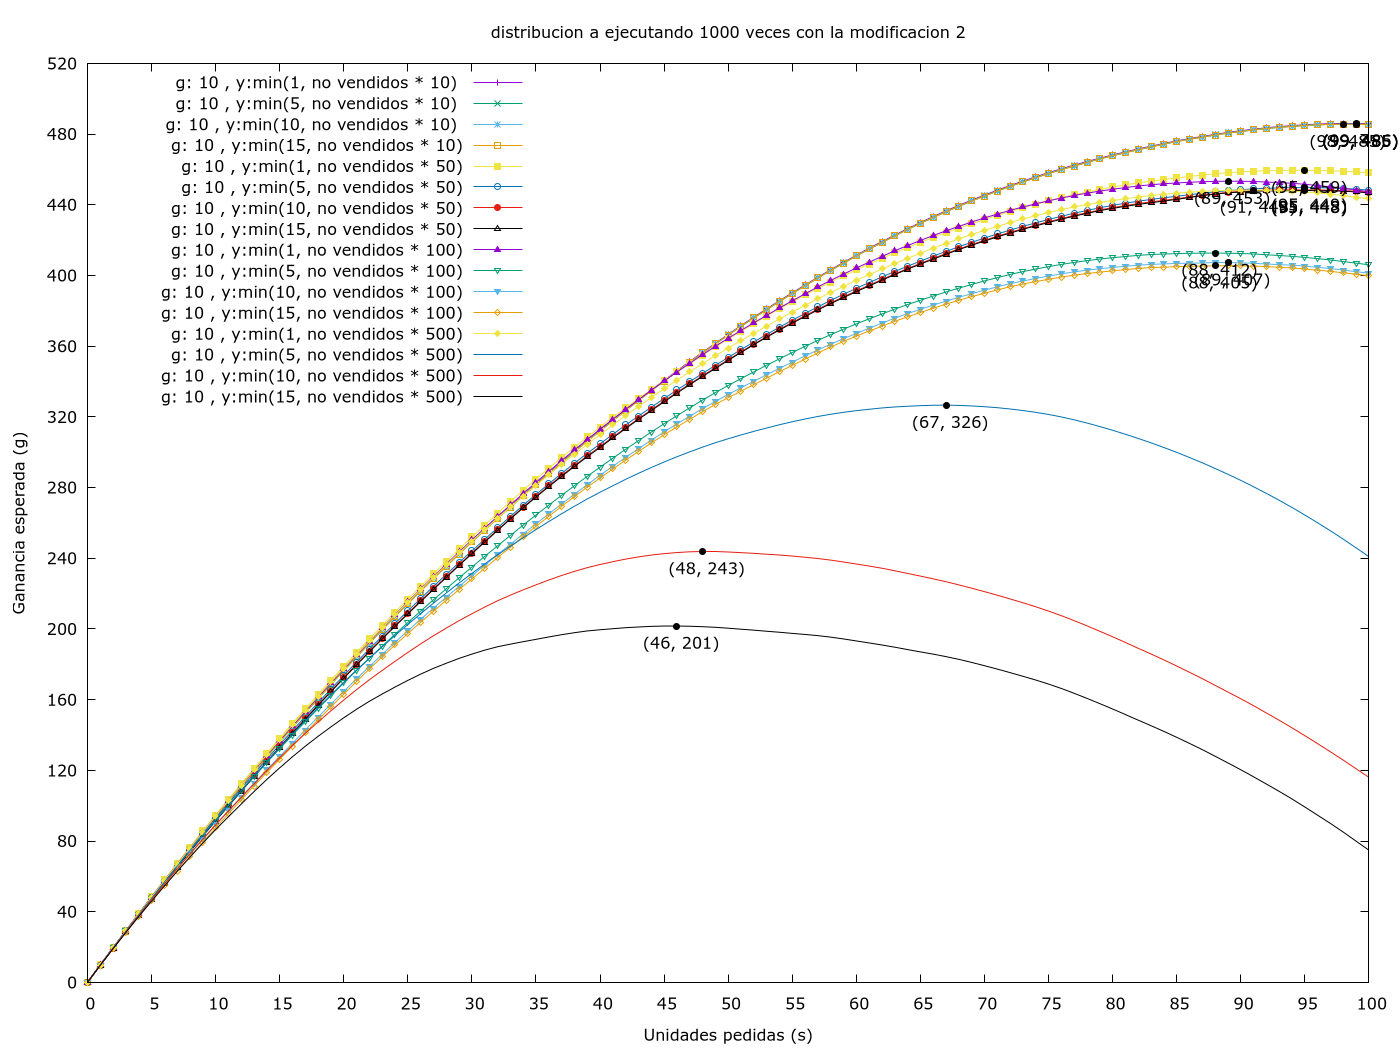
\includegraphics[scale = 0.2]{prob_a/datos_a_1000_2.png}
	\caption{Con 1000 repeticiones, la distribución a y la modificación 2.}
	\label{fig:ej1_a_1000}

\end{figure}

\begin{figure}[H]
	\centering
	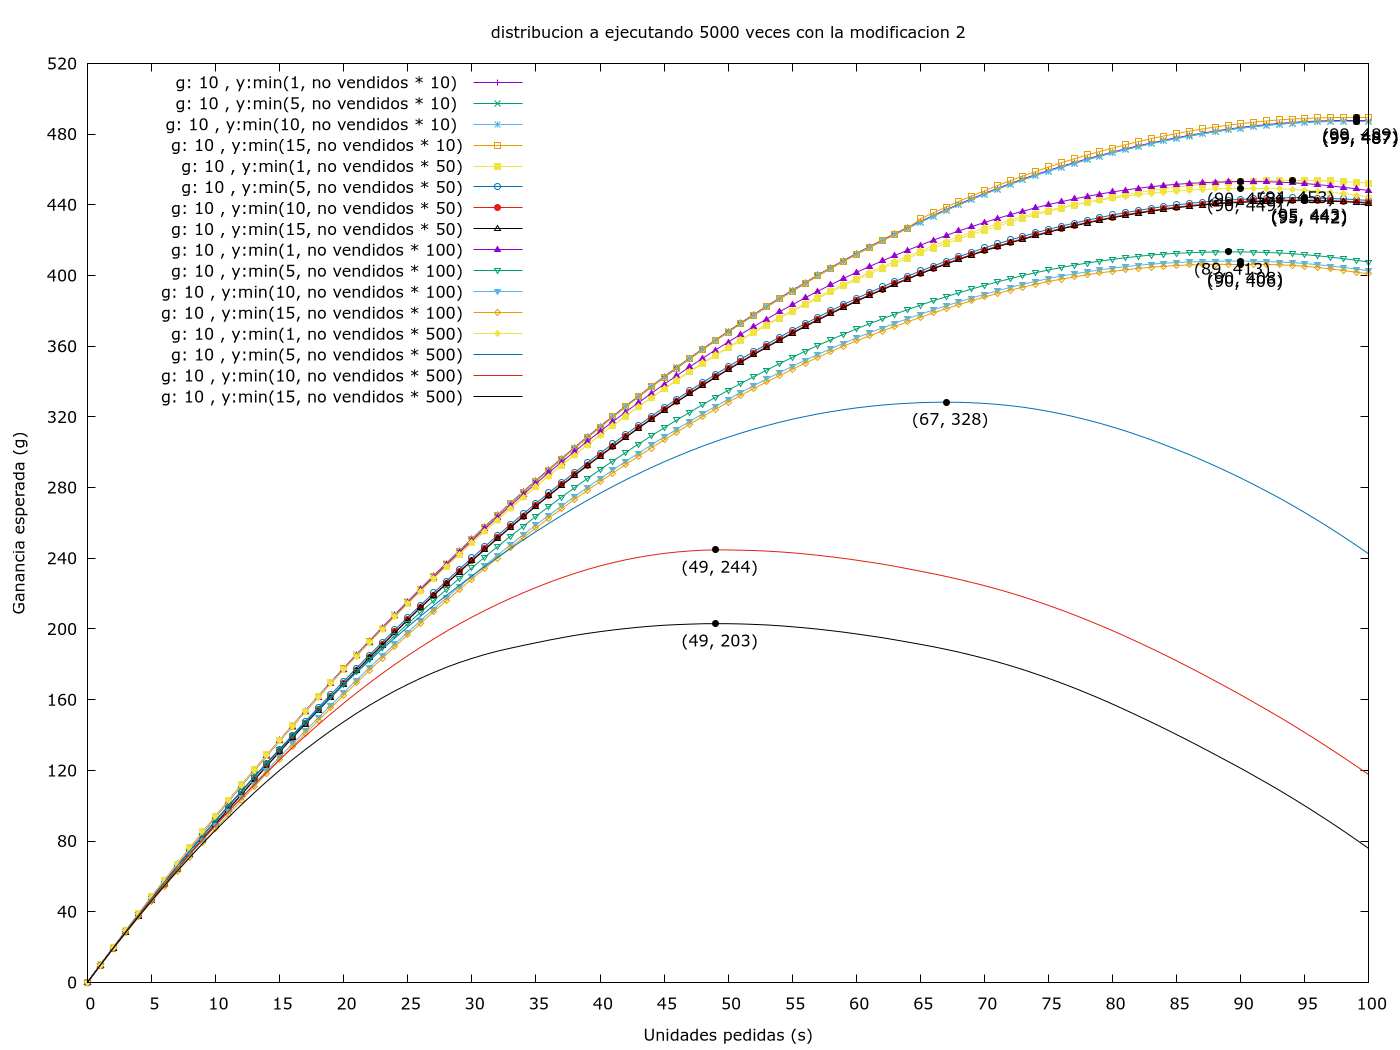
\includegraphics[scale = 0.2]{prob_a/datos_a_5000_2.png}
	\caption{Con 5000 repeticiones, la distribución a y la modificación 2.}
	\label{fig:ej1_a_5000}

\end{figure}


\begin{figure}[H]
	\centering
	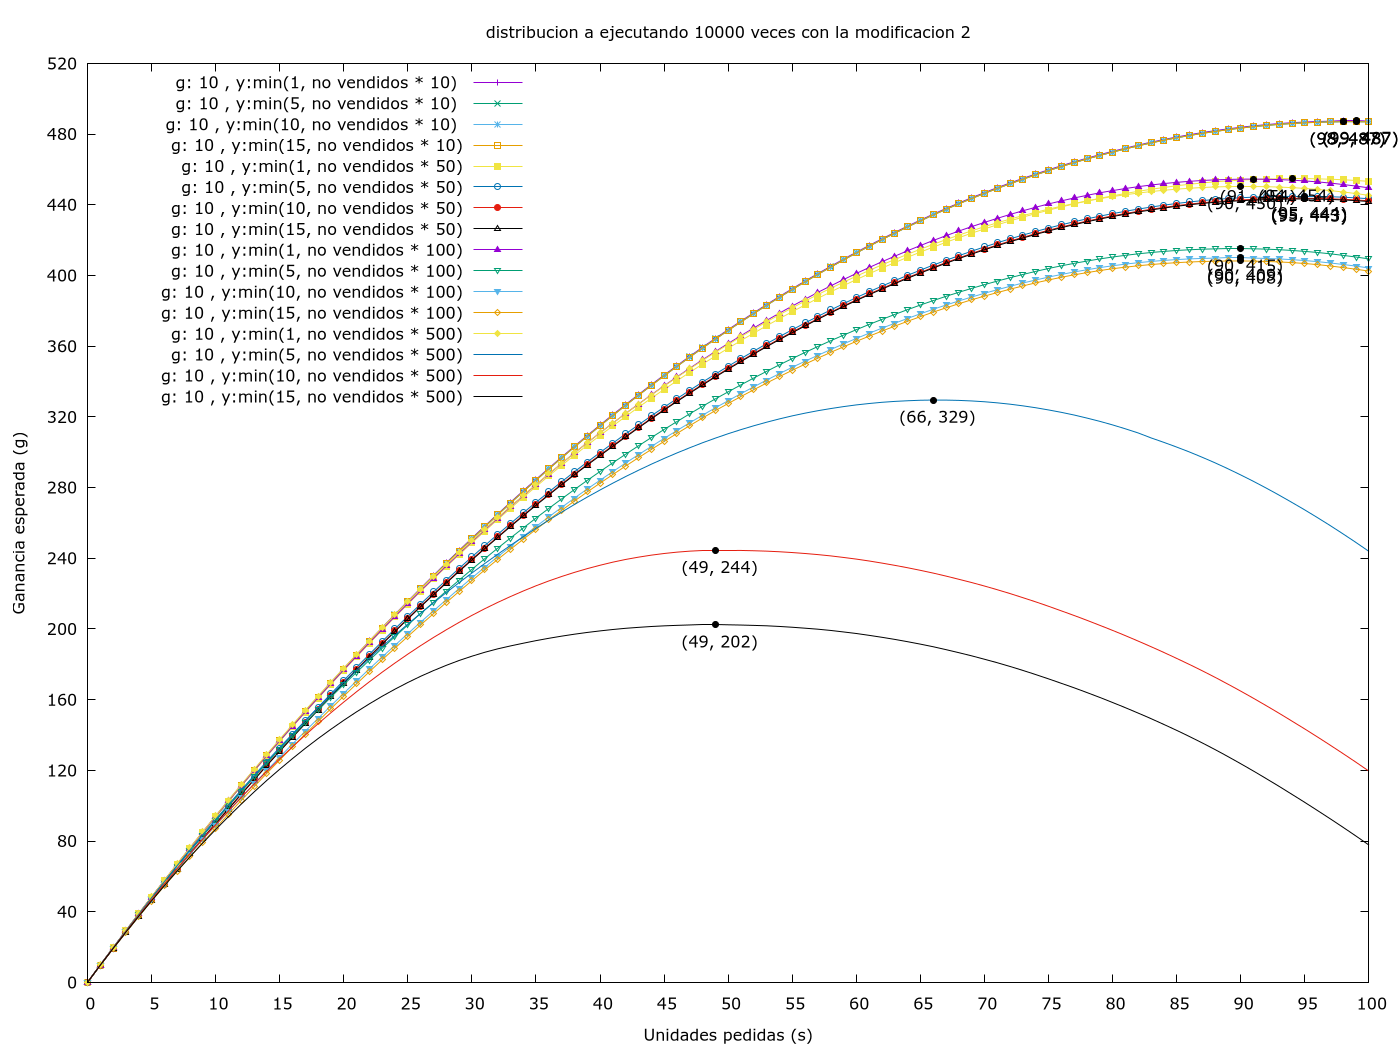
\includegraphics[scale = 0.2]{prob_a/datos_a_10000_2.png}
	\caption{Con 10000 repeticiones, la distribución a y la modificación 2.}
	\label{fig:ej1_a_10000}

\end{figure}

\begin{figure}[H]
	\centering
	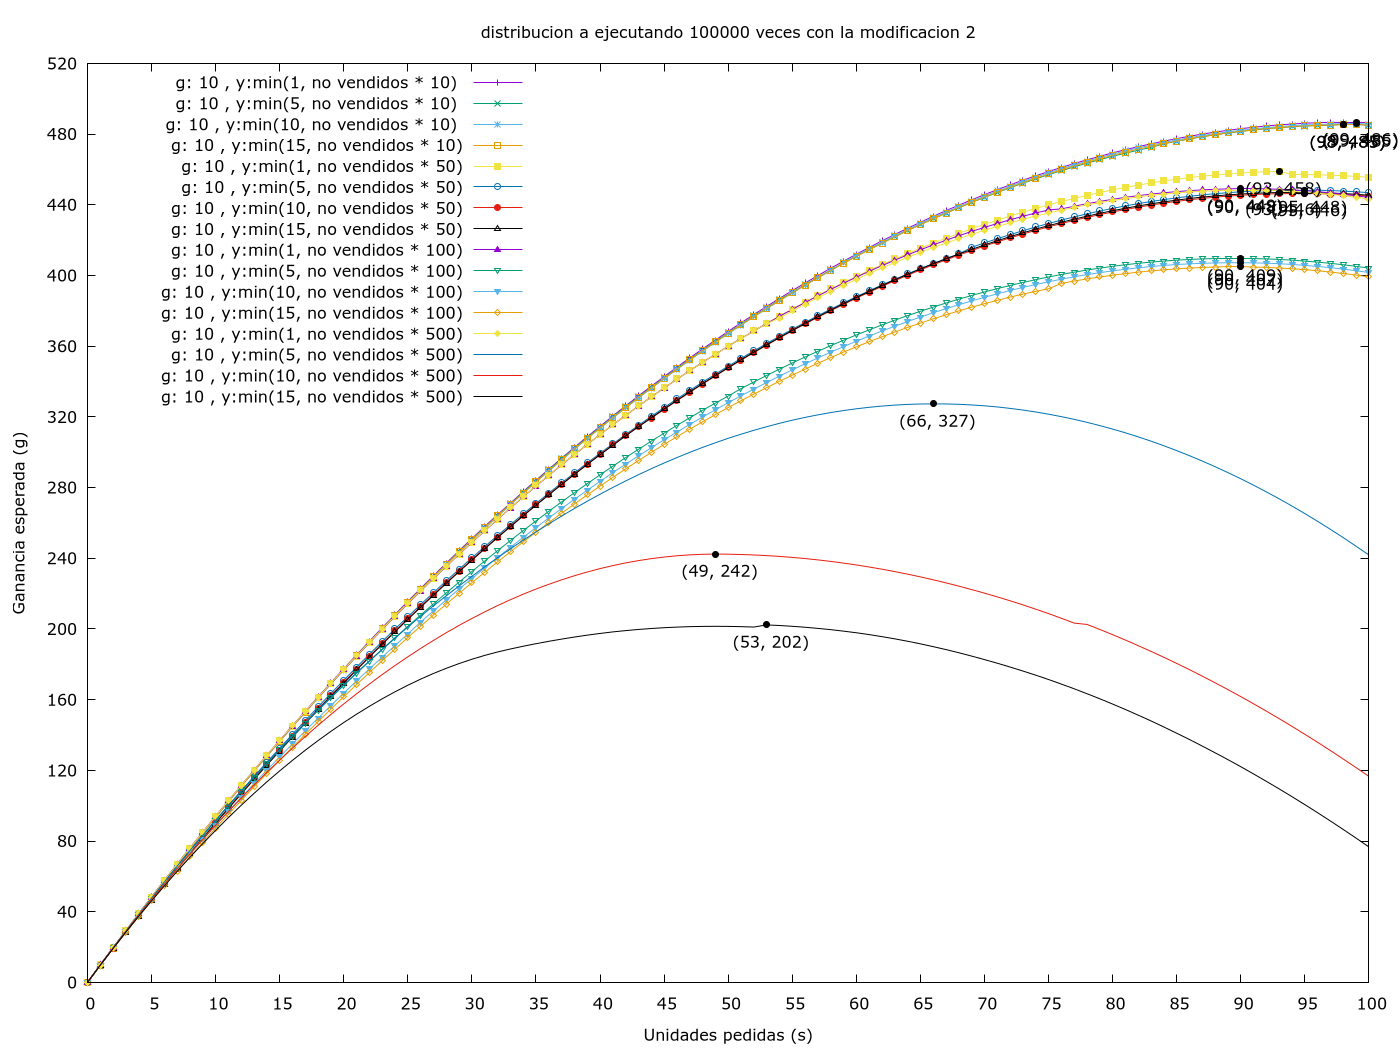
\includegraphics[scale = 0.2]{prob_a/datos_a_100000_2.png}
	\caption{Con 100000 repeticiones, la distribución a y la modificación 2.}
	\label{fig:ej1_a_100000}

\end{figure}

\begin{figure}[H]
	\centering
	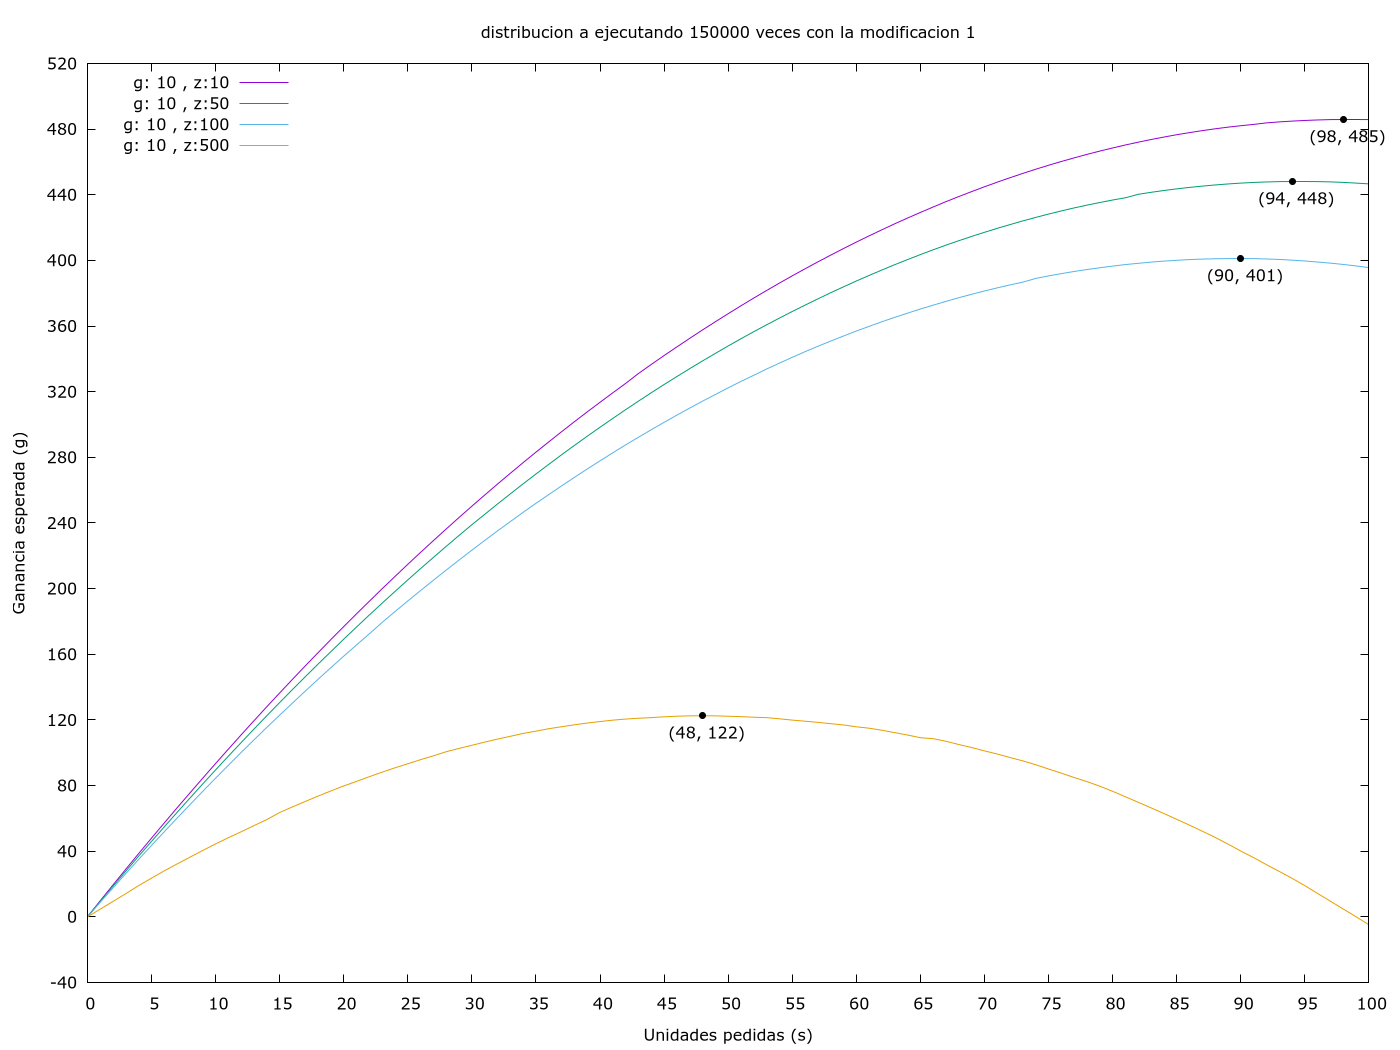
\includegraphics[scale = 0.2]{prob_a/datos_a_150000_1.png}
	\caption{Con 150000 repeticiones, la distribución a y la modificación 1.}
	\label{fig:ej1_a_150000}

\end{figure}


\subsubsection{Resultados obtenidos con la distribución b}


\begin{figure}[H]
	\centering
	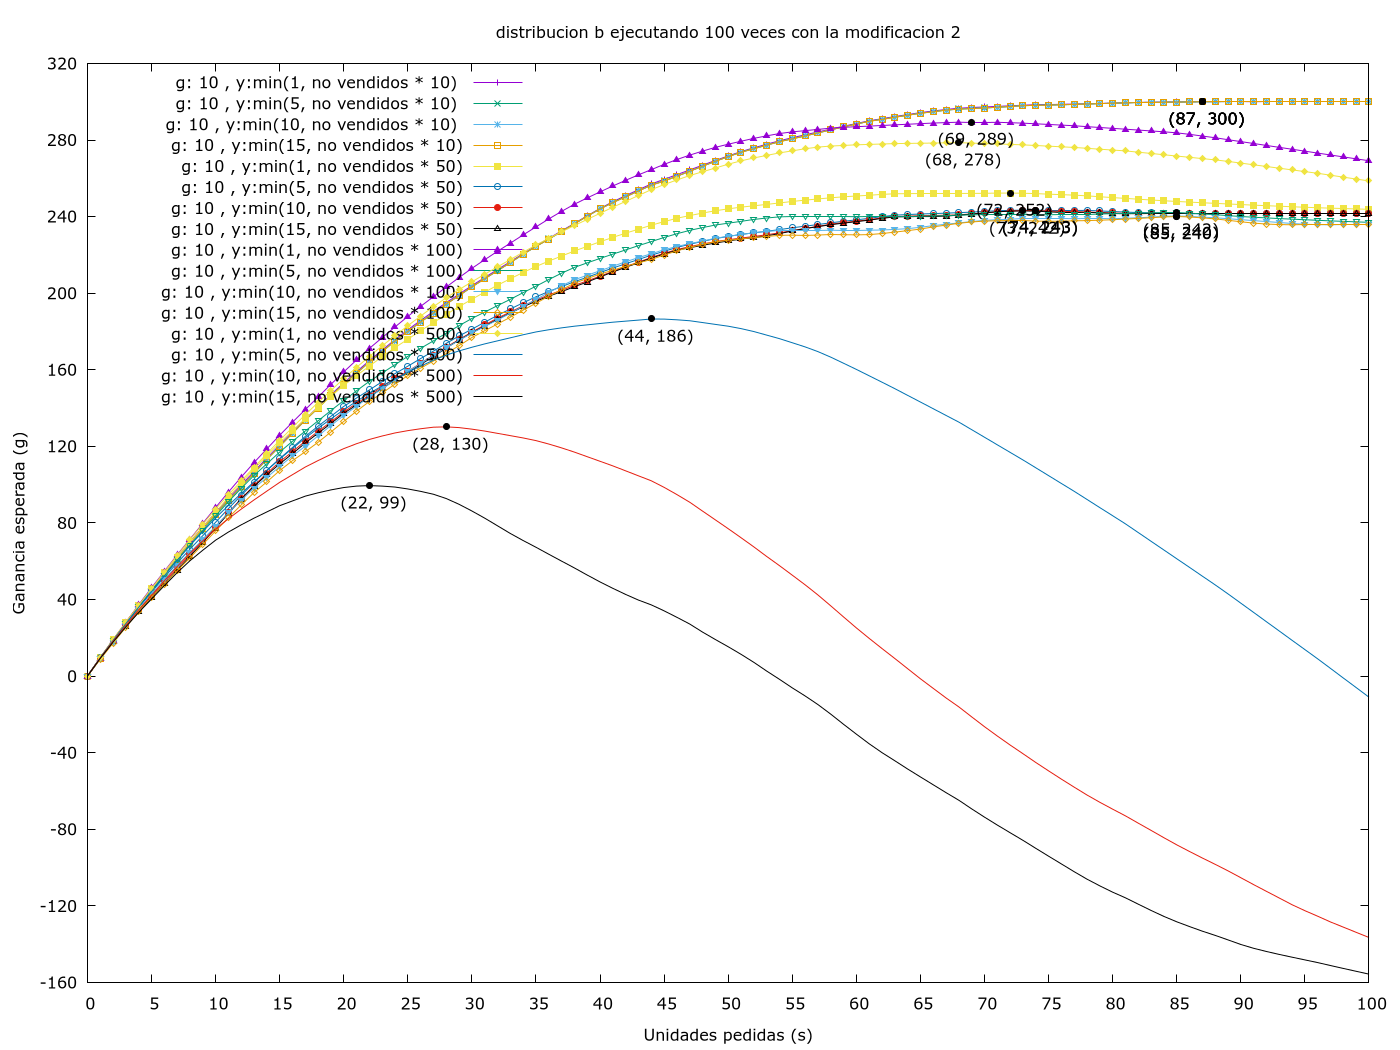
\includegraphics[scale = 0.2]{prob_b/datos_b_100_2.png}
	\caption{Con 100 repeticiones, la distribución b y la modificación 2.}
	\label{fig:ej1_a_100}

\end{figure}

\begin{figure}[H]
	\centering
	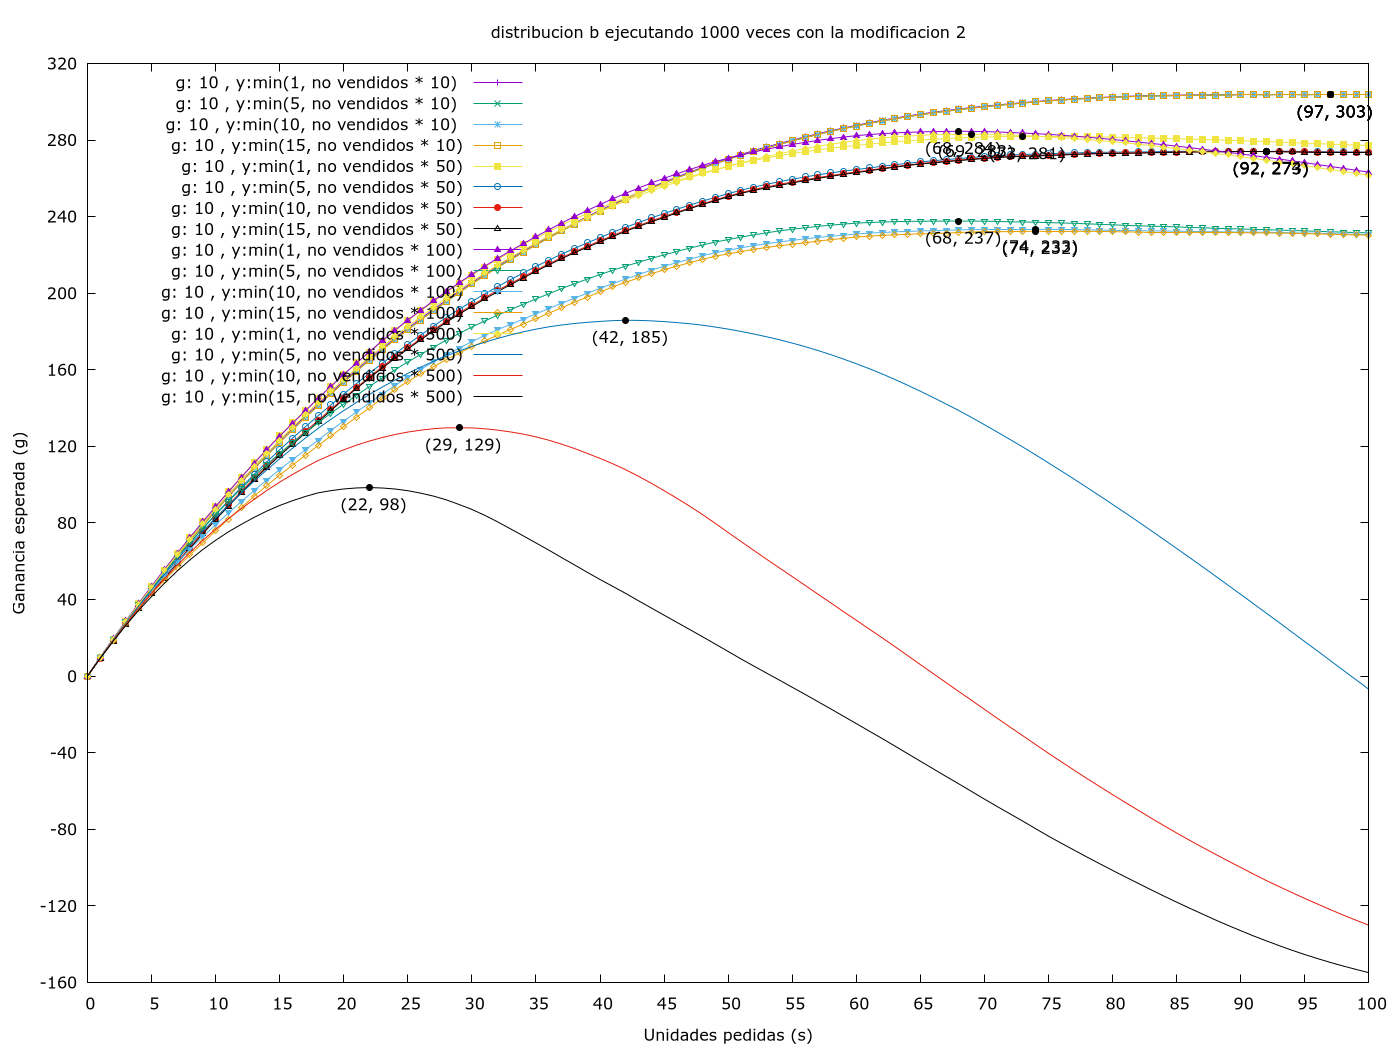
\includegraphics[scale = 0.2]{prob_b/datos_b_1000_2.png}
	\caption{Con 1000 repeticiones, la distribución b y la modificación 2.}
	\label{fig:ej1_a_1000}

\end{figure}

\begin{figure}[H]
	\centering
	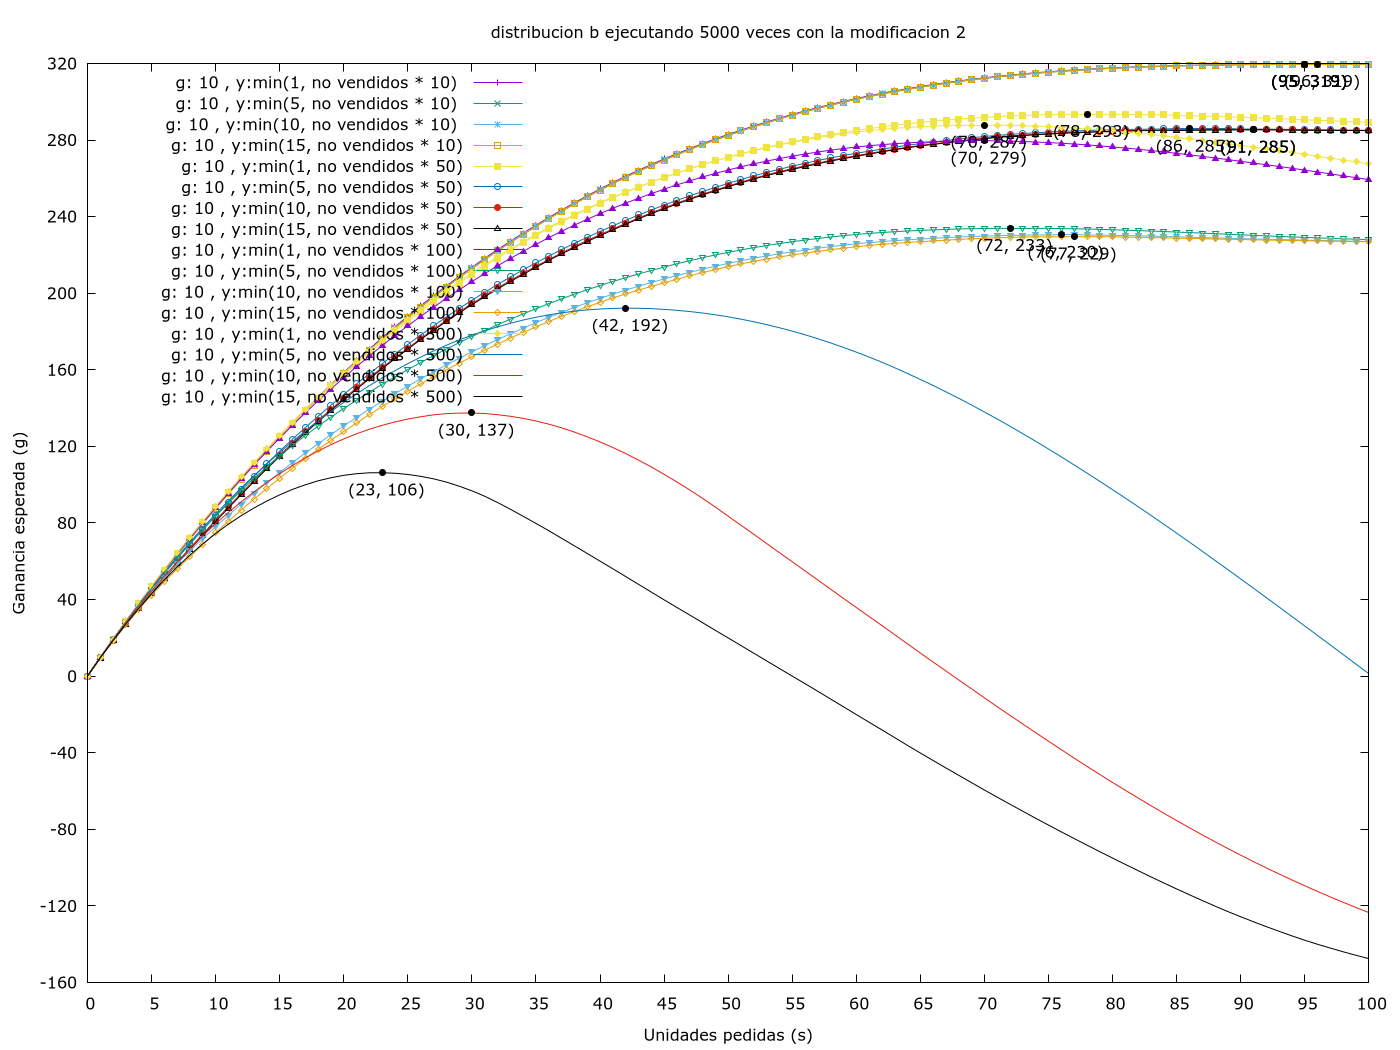
\includegraphics[scale = 0.2]{prob_b/datos_b_5000_2.png}
	\caption{Con 5000 repeticiones, la distribución b y la modificación 2.}
	\label{fig:ej1_a_5000}

\end{figure}


\begin{figure}[H]
	\centering
	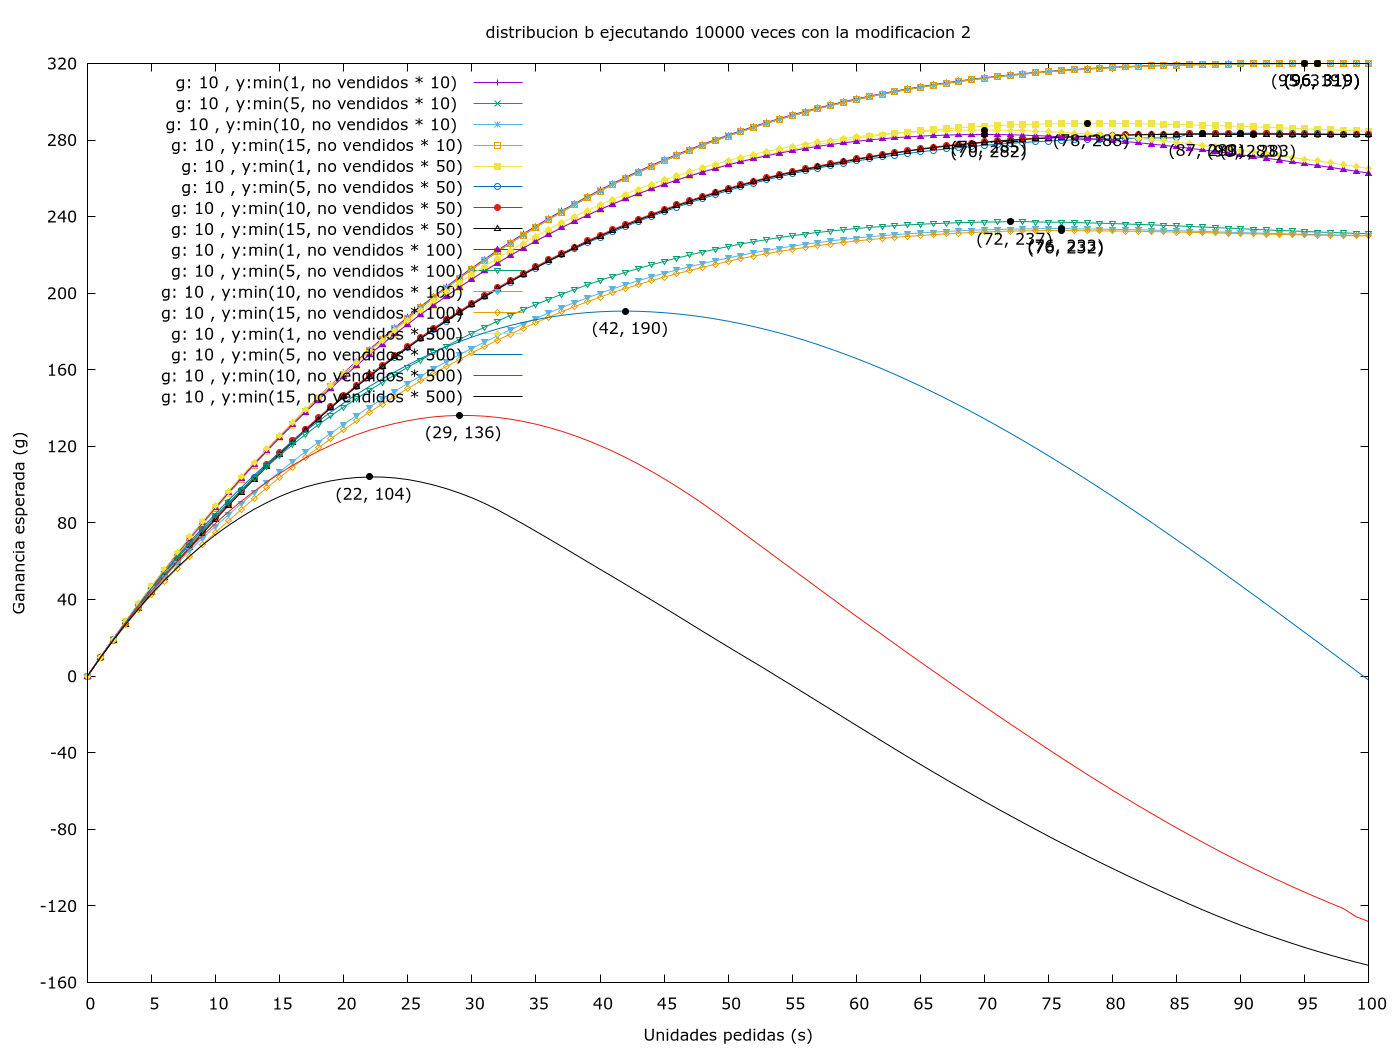
\includegraphics[scale = 0.2]{prob_b/datos_b_10000_2.png}
	\caption{Con 10000 repeticiones, la distribución b y la modificación 2.}
	\label{fig:ej1_a_10000}

\end{figure}

\begin{figure}[H]
	\centering
	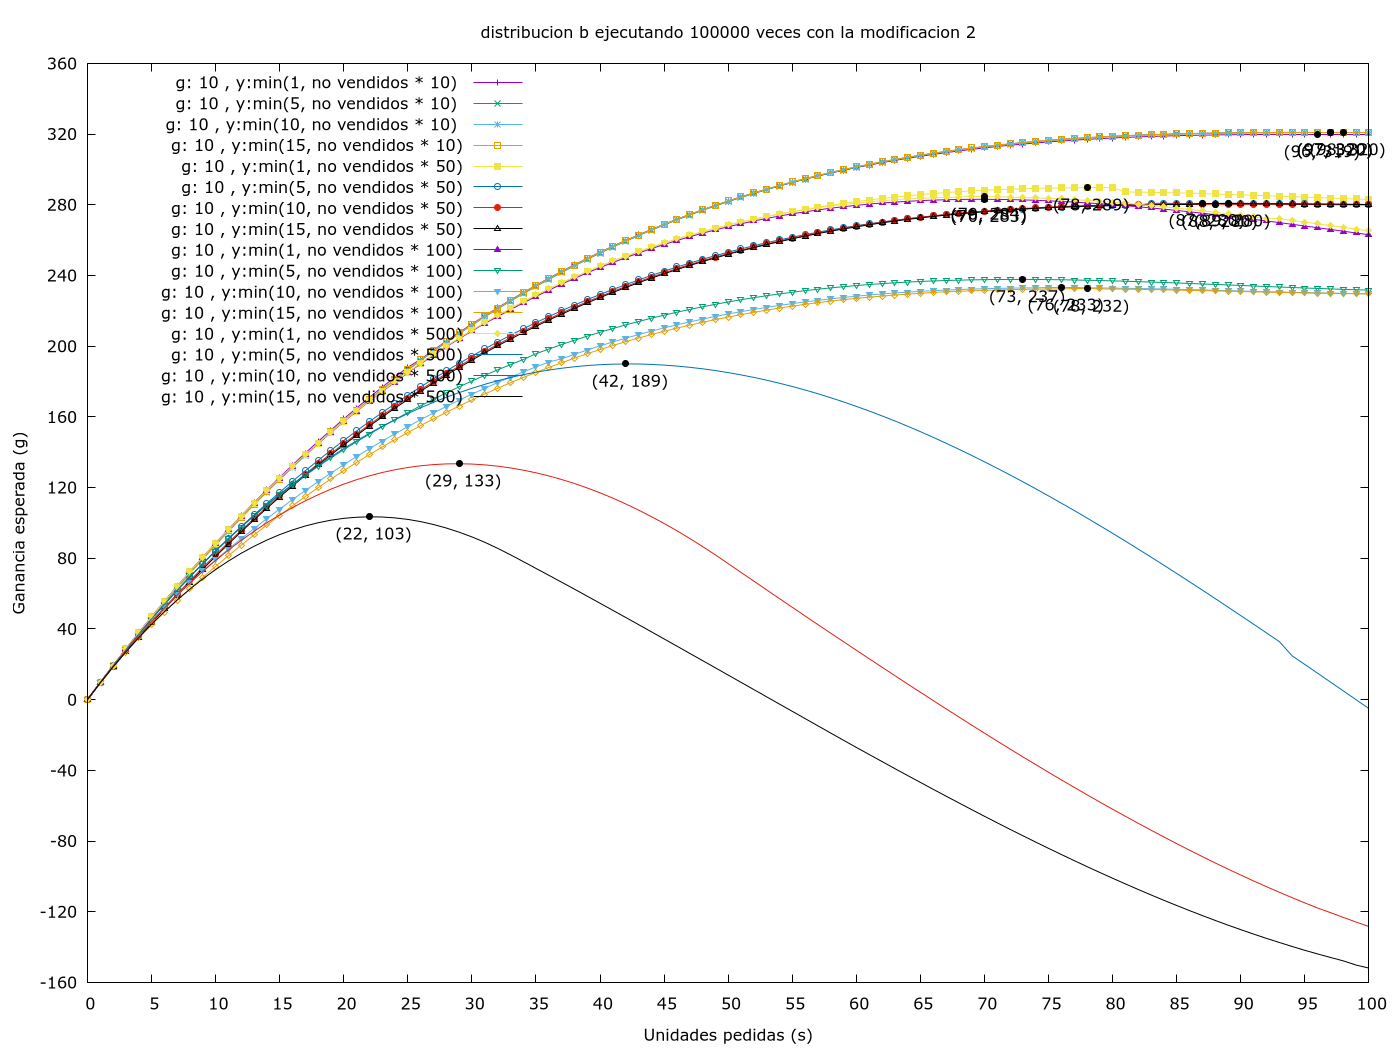
\includegraphics[scale = 0.2]{prob_b/datos_b_100000_2.png}
	\caption{Con 100000 repeticiones, la distribución b y la modificación 2.}
	\label{fig:ej1_a_100000}

\end{figure}

\begin{figure}[H]
	\centering
	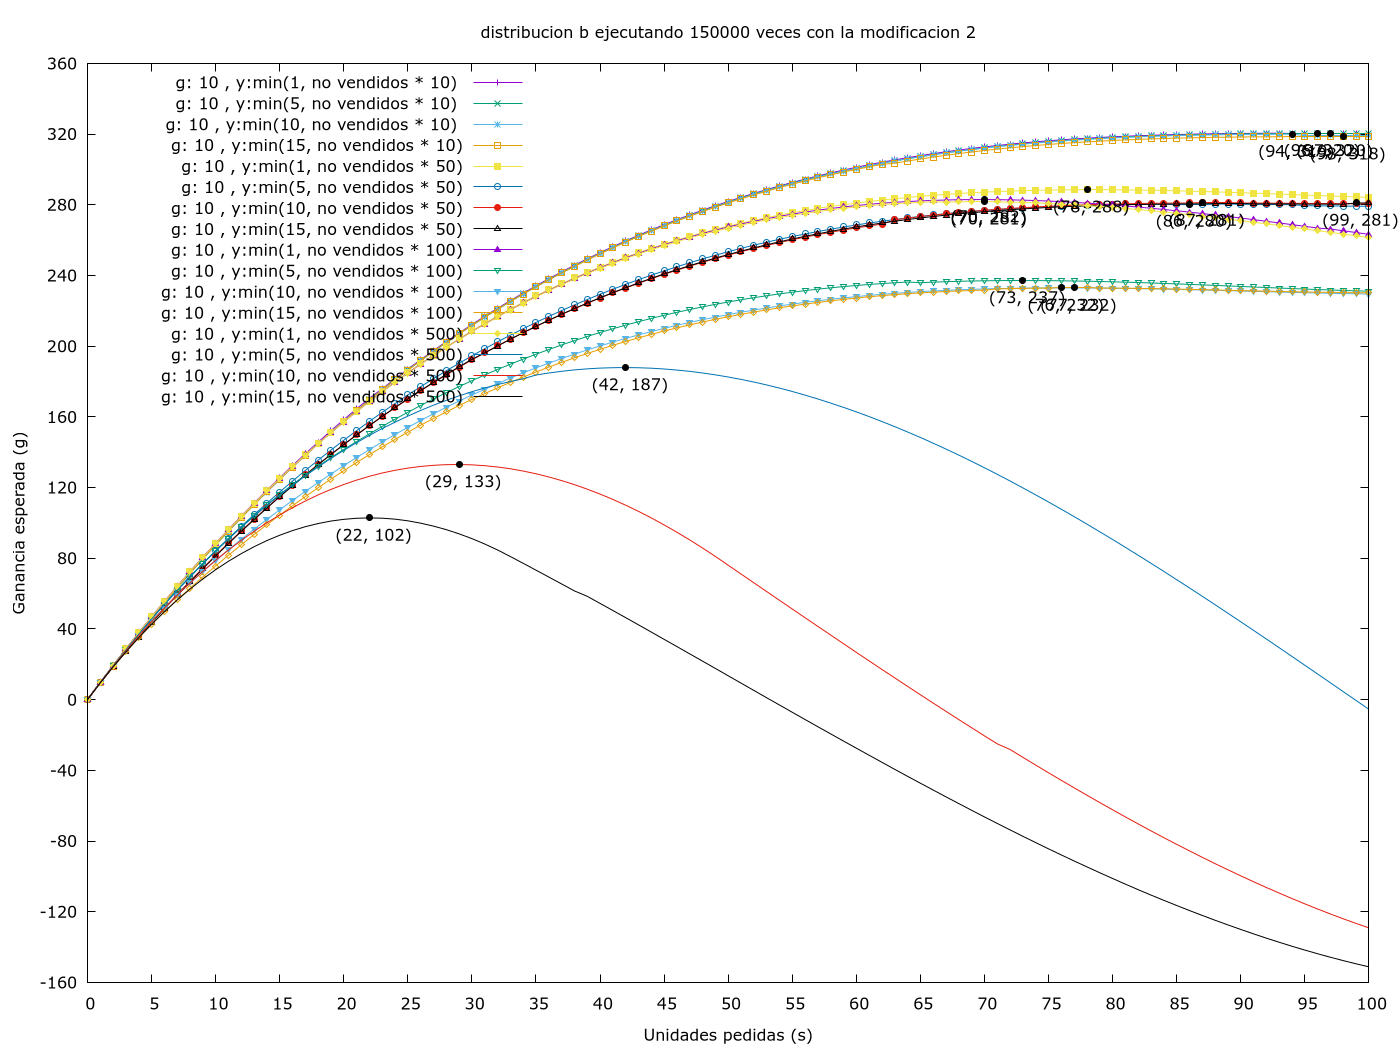
\includegraphics[scale = 0.2]{prob_b/datos_b_150000_2.png}
	\caption{Con 150000 repeticiones, la distribución b y la modificación 2.}
	\label{fig:ej1_a_150000}

\end{figure}

\subsubsection{Resultados obtenidos con la distribución c}

\begin{figure}[H]
	\centering
	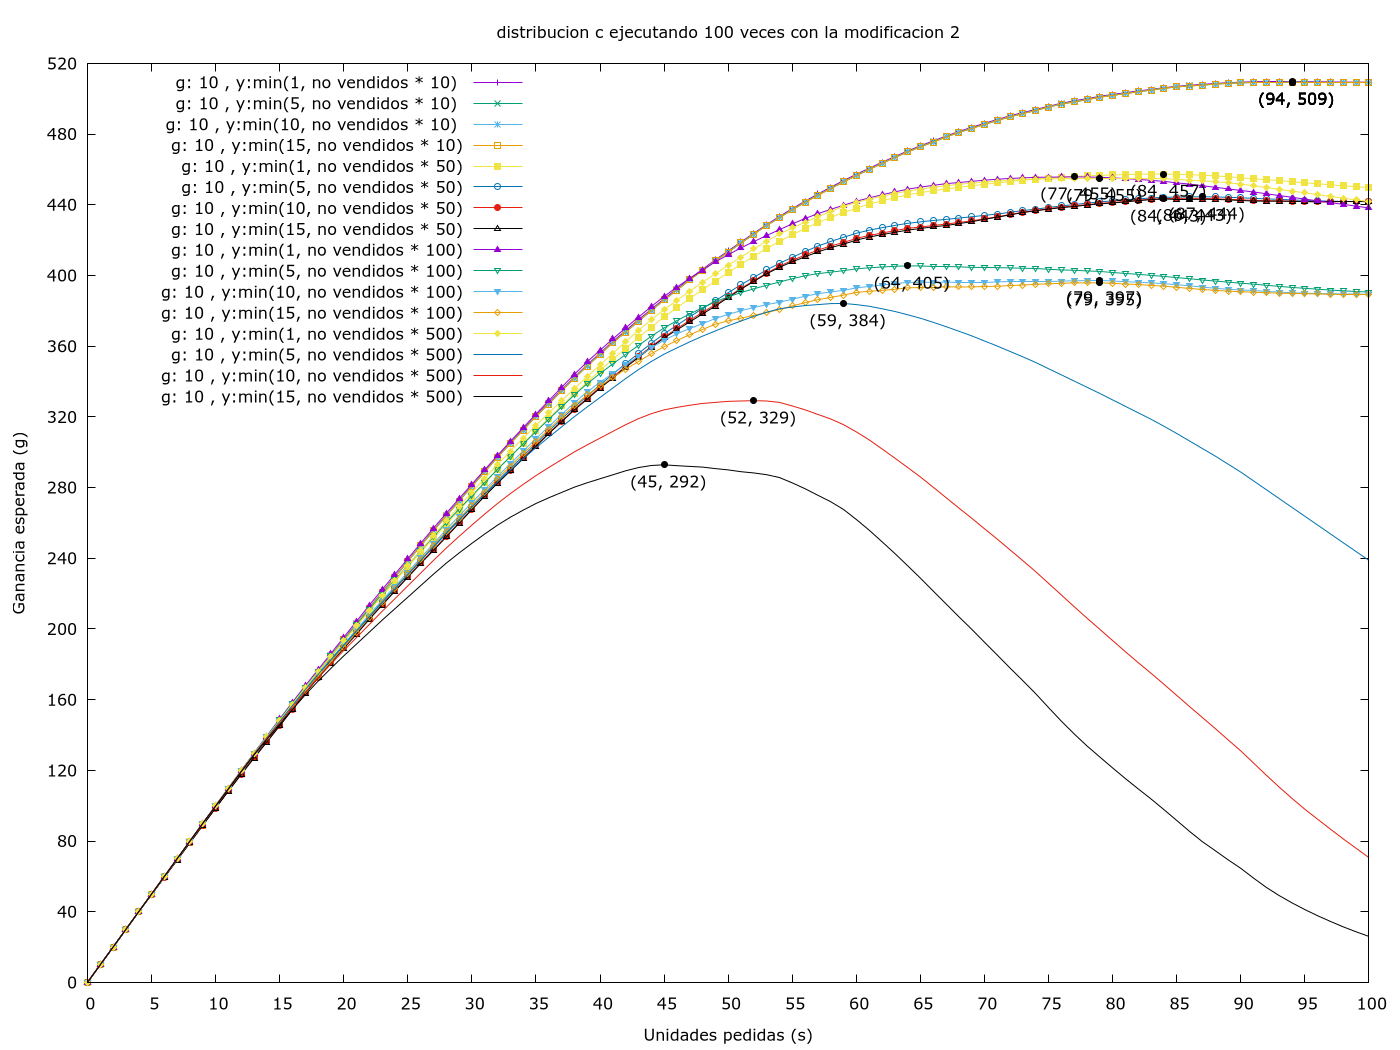
\includegraphics[scale = 0.2]{prob_c/datos_c_100_2.png}
	\caption{Con 100 repeticiones, la distribución b y la modificación 2.}
	\label{fig:ej1_a_100}

\end{figure}

\begin{figure}[H]
	\centering
	\includegraphics[scale = 0.2]{prob_c/datos_c_1000_2.png}
	\caption{Con 1000 repeticiones, la distribución b y la modificación 2.}
	\label{fig:ej1_a_1000}

\end{figure}

\begin{figure}[H]
	\centering
	\includegraphics[scale = 0.2]{prob_c/datos_c_5000_2.png}
	\caption{Con 5000 repeticiones, la distribución b y la modificación 2.}
	\label{fig:ej1_a_5000}

\end{figure}


\begin{figure}[H]
	\centering
	\includegraphics[scale = 0.2]{prob_c/datos_c_10000_2.png}
	\caption{Con 10000 repeticiones, la distribución b y la modificación 2.}
	\label{fig:ej1_a_10000}

\end{figure}

\begin{figure}[H]
	\centering
	\includegraphics[scale = 0.2]{prob_c/datos_c_100000_2.png}
	\caption{Con 100000 repeticiones, la distribución b y la modificación 2.}
	\label{fig:ej1_a_100000}

\end{figure}

\begin{figure}[H]
	\centering
	\includegraphics[scale = 0.2]{prob_c/datos_c_150000_2.png}
	\caption{Con 150000 repeticiones, la distribución b y la modificación 2.}
	\label{fig:ej1_a_150000}

\end{figure}




\section{Generadores de datos}

\subsection{Mejoras de los generadores de datos}

\subsubsection{Reordenación de la tabla de búsqueda}

\begin{figure}[H]
	\centering
	\includegraphics[scale = 0.2]{t_mejora1.png}
	\caption{Reordenando la tabla de búsqueda.}
	\label{fig:ej1_a_150000}

\end{figure}


\subsubsection{Implementación de la búsqueda binaria}

\begin{figure}[H]
	\centering
	\includegraphics[scale = 0.2]{t_mejora2.png}
	\caption{Aplicando una búsqueda binaria en lugar de secuencial.}
	\label{fig:ej1_a_150000}

\end{figure}

\subsubsection{Ejecución en tiempo constante para la distribución a}


\begin{figure}[H]
	\centering
	\includegraphics[scale = 0.2]{t_mejora3.png}
	\caption{Ejecución en tiempo constante para la distribución a.}
	\label{fig:ej1_a_150000}

\end{figure}

\subsection{Implementación de generadores de datos básicos}

\subsubsection{Utilizando aritmética entera}


\subsubsection{Utilizando aritmética real}


\subsubsection{Utilizando aritmética real corregida}



\subsubsection{Utilizando aritmética real con fmod}

% \begin{thebibliography}{9}
%
%
% \end{thebibliography}

\end{document}
